% Modelo de TCC do Bacharelado em Ciência da Computação da UNIFESP 
% Baseado no Modelo de Documentos Academicos do ABNTex2  

\documentclass[	12pt, openright, twoside, a4paper, english, brazil]{abntex2}



% ---
% Pacotes fundamentais 
% ---
\usepackage{cmap}				% Mapear caracteres especiais no PDF
\usepackage{times}
\usepackage[T1]{fontenc}			% Selecao de codigos de fonte.
\usepackage[utf8]{inputenc}		% Codificacao do documento (conversão automática dos acentos)
\usepackage{lastpage}			% Usado pela Ficha catalográfica
\usepackage{indentfirst}			% Indenta o primeiro parágrafo de cada seção.
\usepackage{color}				% Controle das cores
\usepackage{graphicx}			% Inclusão de gráficos
\usepackage{subfig}
\usepackage{minted}
\usepackage{xspace}
\usepackage{setspace}
\usepackage[verbose,a4paper,left=23mm,right=23mm,top=30mm,bottom=23mm]{geometry}
\usepackage{amssymb}
\usepackage{amsmath,amsthm}
\usepackage{url}
\usepackage{fancyvrb}
\usepackage{acronym}
%\usepackage{fancyhdr}
\usepackage{algorithm}
\usepackage{algorithmic}
\usepackage{colortbl}
\usepackage{booktabs}
\usepackage{caption}
\usepackage[table,xcdraw]{xcolor}

\usepackage{listings} % para importação de códigos fonte

% Definindo novas cores
\definecolor{verdecpp}{rgb}{0,0.5,0}
\definecolor{verdejava}{rgb}{0.25,0.5,0.35}
\definecolor{jpurple}{rgb}{0.5,0,0.35}
\definecolor{forestgreen}{RGB}{34,139,34}
\definecolor{orangered}{RGB}{239,134,64}
\definecolor{darkblue}{rgb}{0.0,0.0,0.6}
\definecolor{gray}{rgb}{0.4,0.4,0.4}

\lstdefinestyle{bash}
{
alsolanguage={Bash},
basicstyle=\ttfamily\small,
keywordstyle=\color{blue},
stringstyle=\color{verdecpp},
commentstyle=\color{gray},
extendedchars=true,
showspaces=false,
showstringspaces=false,
%numbers=left,
numberstyle=\tiny,
breaklines=true,
backgroundcolor=\color{green!10},
breakautoindent=true,
captionpos=b,
xleftmargin=0pt,
}

\lstdefinestyle{xml}
{
language={XML},
basicstyle=\ttfamily\small,
stringstyle=\color{jpurple},
commentstyle=\color{gray},
extendedchars=true,
showspaces=false,
showstringspaces=false,
%numbers=left,
numberstyle=\tiny,
breaklines=true,
backgroundcolor=\color{green!10},
breakautoindent=true,
captionpos=b,
xleftmargin=0pt,
morestring=[b]",
morecomment=[s]{<?}{?>},
morecomment=[s][\color{forestgreen}]{<!--}{-->},
keywordstyle=\color{orangered},
tagstyle=\color{darkblue},
morekeywords={attribute,xmlns,version,type,release},
}

% ---
% Pacotes de citações
% ---
\usepackage[brazilian,hyperpageref]{backref}	 % Paginas com as citações na bibl
\usepackage[alf]{abntex2cite}	% Citações padrão ABNT

% --- 
% CONFIGURAÇÕES DE PACOTES
% --- 

% ---
% Configurações do pacote backref
% Usado sem a opção hyperpageref de backref
\renewcommand{\backrefpagesname}{Citado na(s) página(s):~}
% Texto padrão antes do número das páginas
\renewcommand{\backref}{}
% Define os textos da citação
\renewcommand*{\backrefalt}[4]{
	\ifcase #1 %
		Nenhuma citação no texto.%
	\or
		Citado na página #2.%
	\else
		Citado #1 vezes nas páginas #2.%
	\fi}%
% ---

% numeração de figuras e tabelas 
\counterwithout{figure}{section}
\counterwithout{table}{section}

%\renewcommand\tablename{Tabela{\arabic{chapter}.}}


% ---
% Informações de dados para CAPA e FOLHA DE ROSTO
% ---
\titulo{Estudo sobre Computação em Nuvem e análise de desempenho em bases Cassandra}
\autor{Vitor José Camargo de Lima}
\local{São José dos Campos, SP}
\data{Junho de 2015}
\orientador{Prof. Dr. Arlindo Flavio da Conceição}
\instituicao{%
  Universidade Federal de São Paulo -- UNIFESP
  \par
  Instituto de Ciência de Tecnologia
  \par
  Bacharelado em Ciência da Computação}
\tipotrabalho{Trabalho de Graduação}
% O preambulo deve conter o tipo do trabalho, o objetivo, 
% o nome da instituição e a área de concentração 
\preambulo{Trabalho de conclusão de curso apresentado ao Instituto de Ciência e Tecnologia - UNIFESP, como parte das atividades para obtenção do título de Bacharel em Ciência da Computação.}
% ---

% informações do PDF
\makeatletter
\hypersetup{
     	%pagebackref=true,
		pdftitle={\@title}, 
		pdfauthor={\@author},
    	pdfsubject={\imprimirpreambulo},
	    pdfcreator={LaTeX with abnTeX2},
		pdfkeywords={abnt}{latex}{abntex}{abntex2}{trabalho acadêmico}, 
		colorlinks=false,       		% false: boxed links; true: colored links
    	linkcolor=blue,          	% color of internal links
    	citecolor=blue,        		% color of links to bibliography
    	filecolor=magenta,      		% color of file links
		urlcolor=blue,
		bookmarksdepth=4
}

\makeatother
% --- 
% --- 
% Espaçamentos entre linhas e parágrafos 
% --- 
% O tamanho do parágrafo é dado por:
\setlength{\parindent}{1.3cm}
% Controle do espaçamento entre um parágrafo e outro:
\setlength{\parskip}{0.2cm}  % tente também \onelineskip
% ---

% compila o indice
% ---
\makeindex
% ---


% ----
% Início do documento
% ----
\begin{document}
% Retira espaço extra obsoleto entre as frases.
\frenchspacing 

% ----------------------------------------------------------
% ELEMENTOS PRÉ-TEXTUAIS
% ----------------------------------------------------------
%\pretextual


% Capa
\clearpage
\begin{capa}
  \begin{center}
   
\includegraphics[width=.25\textwidth]{imagens/logo-unifesp.pdf}
    \vspace*{\fill}
    
    {\ABNTEXchapterfont\large\imprimirautor}
    \vspace*{\fill}
    
    {\ABNTEXchapterfont\bfseries\Large\imprimirtitulo}
    \vspace*{\fill}\vspace*{\fill}
    
   \imprimirlocal
   \end{center}
\end{capa}



% Folha de rosto
% (o * indica que haverá a ficha bibliográfica)
\imprimirfolhaderosto*


% Folha de aprovação
\clearpage
% Isto é um exemplo de Folha de aprovação, elemento obrigatório da NBR
% 14724/2011 (seção 4.2.1.3). Você pode utilizar este modelo até a aprovação
% do trabalho. Após isso, substitua todo o conteúdo deste arquivo por uma
% imagem da página assinada pela banca com o comando abaixo:
%
% \includepdf{folhadeaprovacao_final.pdf}
%
\begin{folhadeaprovacao}
  \begin{center}
    {\ABNTEXchapterfont\large\imprimirautor}

    \vspace*{\fill}\vspace*{\fill}
    {\ABNTEXchapterfont\bfseries\Large\imprimirtitulo}
    \vspace*{\fill}
    
    \hspace{.45\textwidth}
    \begin{minipage}{.5\textwidth}
        \imprimirpreambulo
    \end{minipage}%
    \vspace*{\fill}
   \end{center}
    
   Trabalho aprovado em 23 de Junho de 2015:

   \assinatura{\textbf{\imprimirorientador} \\ Orientador} 
   \assinatura{\textbf{Prof. Dr. Álvaro Luiz Fazenda} \\ Convidado 1}
   \assinatura{\textbf{Prof. Dra. Denise Stringhini} \\ Convidado 2}
  % \assinatura{\textbf{Professor} \\ Convidado 3}
   %\assinatura{\textbf{Professor} \\ Convidado 4}
      
   \begin{center}
    \vspace*{0.5cm}
    {\large\imprimirlocal}
    \par
    {\large\imprimirdata}
    \vspace*{1cm}
  \end{center}
  
\end{folhadeaprovacao}
% ---


% Dedicatória
%\clearpage
\begin{dedicatoria}
   \vspace*{\fill}
   \centering
   \noindent
   \textit{Dedico este trabalho de conclusão da graduação aos meus pais, irmãos, familiares, esposa e amigos que de muitas formas me incentivaram e ajudaram para que fosse possível a concretização deste trabalho.} \vspace*{\fill}
\end{dedicatoria}


% Agradecimentos
\clearpage
\begin{agradecimentos}


    Agradeço a todas as pessoas do meu convívio que acreditaram e contribuíram, mesmo que indiretamente, para a conclusão deste curso.
Aos meus pais Mara Lúcia Barbosa Camargo de Lima e Joaquim Raimundo de Lima, pelo amor incondicional e pela paciência. Ao meu irmão André Camargo de Lima, que sempre acreditou e me apoiou na concretização da minha graduação. Ao meu irmão Ricardo Alexandre Camargo de Lima, que foi quem me motivou e me ensinou a estudar. 

    À minha esposa Nathalia Cristina de Lima Marton, por compreender a importância dessa conquista, aceitar a minha ausência quando necessário e por me fazer rir e ter esperança em momentos de dificuldade.
Aos amigos Vinicius Fonseca e Vivian Oliveira pelos longos dias de estudos e risadas no corredor da UNIFESP e também pela amizade que ajudou a tornar a vida acadêmica mais divertida.

    Aos amigos, John Godoi, Thiago Rossener, Thiago Furtado, Fábio de Oliveira  e Henrique Miranda, pela ajuda e incentivo durante minha graduação, pelas conversas que muito me ajudaram neste trabalho e pela torcida positiva.
Também ao meu orientador Arlindo Flavio, pelo empenho, paciência e credibilidade. E por fim aos amigos da turma pelas agradáveis lembranças que serão eternamente guardadas em meu coração.

\end{agradecimentos}


% Resumo
\begin{resumo}
Plataformas e \textit{software} estão sendo disponibilizados como serviços em ambientes de Computação em Nuvem com um objetivo, a escalabilidade. Um sistema é descrito como escalável se permanece eficiente quando há um aumento significativo no número de recursos e no número de usuários. Para alcançar escalabilidade, é preciso evitar gargalos no sistema. O objetivo deste trabalho foi estudar modelos de escalabilidade, a partir de conceitos de Computação em Nuvem. Isto inclui realizar estudos sobre ferramentas de virtualização, balanceamento de carga, servidores web, sistema de arquivos distribuídos, entre outras. Foram estudadas diferentes métricas de desempenho para avaliar os modelos, tais como: tempo de resposta, capacidade e eficiência do sistema.
 
 \vspace{\onelineskip}
    
 \noindent
 \textbf{Palavras-chaves}: computação em nuvem, escalabilidade, balanceamento de carga, virtualização.
\end{resumo}


% Abstract
\begin{resumo}[Abstract]
 \begin{otherlanguage*}{english}
 
Systems and software has been launched as services Cloud Computing enviroment with one goal, scability. One system is described as scalable if mantains the efiency when there is a significant rise of quantity of resources and user quantity. In order to achieve scalability, is necessary avoid bottlenecks when running the system. The goal at this work is study scalability, since concepts of Cloud Computing. That includes realize studys about virtualization tools, load balancing, web servers, distribuited file systems, and others subjects. Were studied differents perfomance metrics for evaluate the models, such as : response time, capacity, and efficiency of system in general.

   \vspace{\onelineskip}
 
   \noindent 
   \textbf{Key-words}: Cloud Computing, scalability, load balancing, virtualization.
 \end{otherlanguage*}
\end{resumo}


% Lista de ilustrações
\pdfbookmark[0]{\listfigurename}{lof}
\listoffigures*
\cleardoublepage


% Lista de tabelas
\pdfbookmark[0]{\listtablename}{lot}
\listoftables*
\cleardoublepage


% Lista de abreviaturas e siglas
\clearpage
\begin{siglas}
    \item[API] Interface de Programação de Aplicativos (\textit{Application  Programming  Interface})
     \item[CISCS] Computador com um Conjunto Complexo de Instruções (\textit{Complex Instruction Set Computer})
    \item[CPU] Unidade Central de Processamento (\textit{Central Processor Unit}) 
    \item[DNS] Sistema de Nomes de Domínios (\textit{Domain Name System})
    \item[I/O] Entrada/Saída de dados (\textit{Input/Output of data})
    \item[IEEE] Instituto de Engenheiros Eletricistas e Eletrônicos (\textit{Institute of Electrical and Electronics Engineers})
    \item[MFLOPS] Milhões de Instruções de Ponto Flutuante Por Segundo (\textit{Millions of Floating Point Instructions Per Second})
     \item[MIPS] Milhões de Instruções Por Segundo (\textit{Millions of Instructions Per Second})
     \item[MTU] Unidade Máxima de Transmissão (\textit{Maximum Transmission Unit})
  \item[NAT] Tradução de Endereços de Rede (\textit{Network Address Translation})
    \item[POSIX] Interface Portável entre Sistemas Operacionais (\textit{Portable Operating System Interface})
     \item[QEMU] emulador de software (emulador de processador ou outro subsistema necessário) baseado na tradução dinâmica de binários
     \item[RISCS] Computador com um Conjunto Reduzido de Instruções (\textit{Reduced Instruction Set Computer})
     \item[SO] Sistema Operacional
  \item[VLAN] Rede Local Virtual (\textit{Virtual LAN})
\end{siglas}


% Sumario
\pdfbookmark[0]{\contentsname}{toc}
\tableofcontents*
\cleardoublepage


% ----------------------------------------------------------
% ELEMENTOS TEXTUAIS
% ----------------------------------------------------------
\textual


% Introdução
\chapter{Introdução}
\label{cap:introducao}
Computação em Nuvem é atualmente um dos principais tópicos em sistemas distribuídos. As novas formas de oferecer serviços de software tem atraído as empresas e a sociedade. Segundo \citeonline{JISA2010}, isto se deve a vários fatores, como:

\begin{itemize}
    \item baixo investimento inicial;
    \item redução de custos operacionais;
    \item escalabilidade;
    \item redução de riscos e despesas de manutenção.
\end{itemize}

Num estudo realizado em 2013, os analistas da Frost \& Sullivan, empresa global de consultoria especializada em estratégia de crescimento, concluíram que o mercado brasileiro de computação esta mais adepto a Computação em Nuvem que os demais mercados do mundo. Dados extraídos da pesquisa realizada em São Paulo mostram que 39\% das companhias que atuam na América Latina possuem aplicativos hospedados na nuvem \cite{Silva2014}.

Desta forma, saber avaliar e definir qual estratégia de escalabilidade a ser utilizada, tem sido cada vez mais importante na Computação em Nuvem. Tais estratégias representam ganhos significativos para a expansão dos serviços e recursos oferecidos \cite{JISA2011}.

Pode-se citar a Amazon Web Services (AWS) como exemplo de empresa que investiu na Computação em Nuvem desde 2006 e hoje este é o seu principal serviço. Esta empresa desenvolveu uma plataforma que facilita e viabiliza o uso da tecnologia em nuvem, fazendo com que milhares de empresas migrassem seus serviços para os seus servidores, como por exemplo: Novartis, Nokia, Pfizer, Adobe, Netflix, entre outras \cite{AmazonWebServices2015}. Conforme estudo realizado pela Netflix e citado na seção \ref{sec:cassjmeter}, os testes realizados na plataforma Amazon revelam que os serviços da Netflix conseguiram atender a um maior número de clientes a medida que se aumenta a escalabilidade da nuvem. 

A utilização da virtualização nestes sistemas permite que um hardware seja utilizado para executar vários sistemas operacionais ao mesmo tempo, sejam eles sistemas iguais ou diferentes, visando o máximo aproveitamento dos recursos computacionais. Com isso, pode-se ter diversas redes privadas dentro de um mesmo servidor. Para garantir segurança, desempenho e confiabilidade destas redes são utilizados diversos tipos de isolamento e de configurações.

Dentro destas redes e sistemas virtuais, os dados são geralmente armazenados em um banco de dados NoSQL, distribuído e rápido, com o qual é possível trabalhar com grande volume de dados. Desta forma, o banco de dados escolhido para ser estudado neste trabalho foi o Cassandra. Ele é um banco de dados baseado no tipo chave/valor, onde os dados são identificados através de uma chave e cujas principais características são: escalabilidade, disponibilidade, tolerância a falhas e tempo de resposta rápido \cite{Silva}.

Sendo assim, neste trabalho, foram investigados produtos utilizados para alcançar escalabilidade e os ambientes computacionais ditos escaláveis. Também foram realizadas simulações de escalabilidade no banco de dados para os serviços oferecidos pelo projeto Maritaca \cite{maritaca}. Nos quais foram avaliados o comportamento do sistema em relação ao volume de dados e tráfego, quando estes aumentam ou diminuem, e à detecção de gargalos. Para tais avaliações, utilizou-se o JMeter e o CassJMeter para simular o funcionamento do sistema a ser avaliado e realizar os testes na base Cassandra.

Para isto, este trabalho foi organizado da seguinte forma: o capítulo \ref{cap:fundTeorica} aborda conceitos de Computação em Nuvem, diferenciando os tipos de serviços e principais estruturas. O capítulo \ref{cap:ferramentas} descreve as ferramentas utilizadas neste trabalho. O capítulo \ref{cap:ambExperimental} detalha o servidor utilizado para criação dos ambientes experimentais e os modelos de escalabilidade, bem como alguns diagramas que exemplificam conceitos como: redes virtuais, redes privadas, isolamento de redes, balanceamento de carga e o relacionamento entre estes. O detalhamento de bases Cassandra operando em \textit{cluster} e o plano de testes das mesmas estão descritos no capítulo \ref{cap:cassandra}. A seleção de técnicas e métricas para análise de desempenho, bem como as métricas mais usadas são apresentadas no capítulo \ref{cap:analisePerformance}. No capítulo \ref{cap:resultados} são tratados os assuntos relacionados aos resultados obtidos. No capítulo \ref{cap:dificuldadesEncontradas}, são apresentadas as principais dificuldades encontradas na execução deste trabalho e no capítulo \ref{cap:conclusoes} é feito um fechamento recapitulando pontos importantes discutidos ao longo do trabalho e as conclusões obtidas.


% Fundamentação Teórica
\chapter{Revisão sobre Computação em Nuvem}
\label{cap:fundTeorica}
Este capítulo apresenta as principais definições e conceitos relacionados com a Computação em Nuvem, tais como: as características essenciais, os tipos de serviço, os tipos de implantação e alguns conceitos e ferramentas importantes para a funcionamento da nuvem.


A Computação em Nuvem (\textit{Cloud Computing}) é uma tecnologia que permite oferecer acesso remoto a software e executar diversas tarefas utilizando a Internet. Ela representa a infraestrutura de comunicação entre os componentes arquiteturais, baseada em uma abstração que oculta à complexidade de infraestrutura. Cada parte desta infraestrutura é provida como um serviço utilizando hardware compartilhado para computação e armazenamento.
Neste capítulo, serão definidas as características essenciais, os tipos de serviço, os tipos de implantação e uma definição resumida dos principais conceitos e ferramentas utilizadas na Computação em Nuvem \cite{ERCEMAPI2009}. 

\begin{quote}
\textit{"O modelo de computação em nuvem foi desenvolvido com o objetivo de fornecer serviços de fácil acesso, baixo custo e com garantias de disponibilidade e escalabilidade. Este modelo visa fornecer, basicamente, três benefícios. O primeiro benefício é reduzir o custo na aquisição e composição de toda infraestrutura requerida para atender as necessidades das empresas, podendo essa infraestrutura ser composta sob demanda e com recursos heterogêneos e de menor custo. O segundo é a flexibilidade que esse modelo oferece no que diz respeito à adição e substituição de recursos computacionais, podendo escalar tanto em nível de recursos de hardware quanto software para atender as necessidades das empresas e usuários. O último benefício é prover uma abstração e facilidade de acesso aos usuários destes serviços. Neste sentido, os usuários dos serviços não precisam conhecer aspectos de localização física e de entrega dos resultados destes serviços"} \cite{ERCEMAPI2009}.
\end{quote}

\section{Características Essenciais}

Pode-se definir e diferenciar a Computação em Nuvem de outros paradigmas quando combina-se algumas de suas características. Por exemplo, a elasticidade rápida de recursos, amplo acesso e a medição de serviço são características essenciais para compor uma solução de Computação em Nuvem \cite{ERCEMAPI2009}.

As características essenciais da Computação em Nuvem são:

\begin{itemize}
  \item Requisição de serviço sob demanda: o usuário pode adquirir unilateralmente recurso computacional na medida em que necessite e sem precisar de interação humana com os provedores de cada serviço, como tempo de procesamento no servidor ou armazenamento na rede. A infraestrutura dentro de uma nuvem podem ser automaticamente reconfigurada e/ou modificada e estas ações são transparentes para os usuários \cite{ERCEMAPI2009}.
  
  \item Amplo acesso: recursos são disponibilizados via Internet e acessados por meio de mecanismos padronizados que possibilitam o uso com plataformas \textit{thin}, tais como celulares, \textit{laptops} e PDAs. A interface de acesso à nuvem não obriga os usuários a mudar suas condições e ambientes de trabalho, como por exemplo, linguagens de programação e sistema operacional \cite{ERCEMAPI2009}.
  
  \item Portifólio de Recursos: os recursos computacionais do provedor são disponibilizados para servir múltiplos usuários usando um modelo \textit{multi-tenant} ou multi-inquilino, com diferentes recursos físicos e virtuais, dinamicamente atribuídos e ajustados de acordo com a demanda dos usuários. Estes usuários não precisam ter conhecimento da localização física dos recursos computacionais, podendo somente especificar a localização em um nível mais alto de abstração, tais como o país, estado ou centro de dados \cite{ERCEMAPI2009}.
  
  \item Elasticidade Rápida: recursos podem ser adquiridos de forma rápida e elástica. Em alguns casos automaticamente, se houver a necessidade de aumentar a quantidade disponibilizada de recursos, dado o aumento da demanda. Além disso, pode ser realocado quando há retração dessa demanda. Para os usuários, os recursos disponíveis parecem ser ilimitados e podem ser adquiridos em qualquer quantidade e a qualquer momento. A virtualização auxilia a elasticidade rápida ao criar várias instâncias de recursos requisitados utilizando um único recurso real. É através da virtualização que se pode abstrair características físicas de uma plataforma computacional dos usuários, exibindo outro hardware virtual e emulando um ou mais ambientes que podem ser independentes ou não \cite{ERCEMAPI2009}.
  
  \item Serviço Medido: sistemas em nuvem controlam e otimizam, automaticamente, o uso de recursos por meio de uma capacidade de medição. A automação é realizada em algum nível de abstração apropriado para o tipo de serviço, tais como armazenamento, processamento, largura de banda e contas dos usuários ativos. O uso de recursos pode ser monitorado e controlado, possibilitando transparência para o provedor e o usuário do serviço utilizado. Para garantir a qualidade do serviço, ou \textit{Quality of Service} (QoS), pode-se utilizar a abordagem baseada em acordo de nível de serviço, ou \textit{Services Level Agreement} (SLA). O SLA fornece informações sobre os níveis de disponibilidade, funcionalidade, desempenho e pode até mesmo estabelecer penalidades em caso de violação destes níveis \cite{ERCEMAPI2009}.
  
\end{itemize}

\section{Tipos de Serviço}
De acordo com \cite{JISA2010}, o modelo de negócios orientado a serviços é dividido em:

\begin{itemize}
  \item Software como Serviço (Saas): a aplicação é disponibilizada via Internet para que o cliente utilize conforme sua necessidade;
  \item Plataforma como Serviço (Paas): oferece partes de um ambiente ou de um sistema operacional completo, de forma que os usuários possam acessá-los remotamente;
  \item Infraestrutura como serviço (Iaas): objetivo é oferecer a infraestrutura de hardware de forma remota e transparente.
\end{itemize}

A Figura \ref{fig:modelo-servicos} exibe os tipos de serviços oferecidos na Computação em Nuvem e os relacionamentos entre eles.

\begin{figure}[H]
\centering
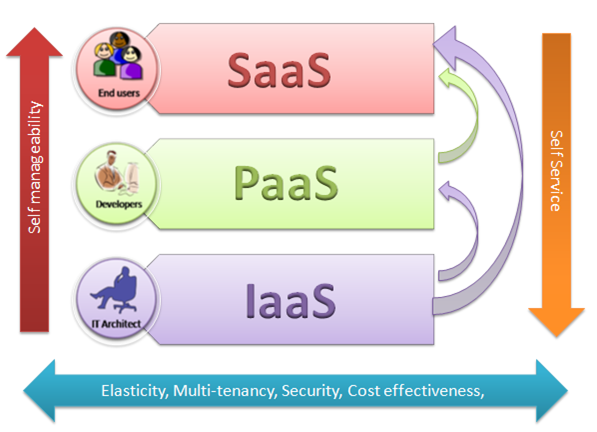
\includegraphics[scale=1]{imagens/delivery_models.png}
\caption{Modelos de Serviços em Computação em Nuvem}\cite{Alhamad2010}
\label{fig:modelo-servicos}
\end{figure}

\section{Tipos de implantação}
Pode-se classificar a estrutura disponível para os ambientes de computação em nuvem, em quatro diferentes tipos:

\begin{itemize}
  \item Público: Uma nuvem em que os prestadores de serviços oferecem seus recursos como serviços para o público em geral. As nuvens públicas oferecem vários benefícios importantes, incluindo nenhum investimento inicial em infraestrutura e deslocamento dos riscos para os fornecedores de infraestrutura. No entanto, a falta de controle refinado sobre as definições de dados, rede e segurança dificulta a eficácia em muitos cenários de negócios \cite{JISA2010}.
  
  \item Privado:  Também conhecido como nuvens internas, as nuvens privadas são projetadas para uso exclusivo por uma única organização. Uma nuvem privada pode ser construída e gerida pela organização ou por provedores externos. Esta oferece o mais alto grau de controle sobre o desempenho, confiabilidade e segurança. No entanto, são semelhantes à servidores proprietários tradicionais e não oferecem benefícios como redução nos custos de capital inicial \cite{JISA2010}.
  
  \item Híbrido: Uma nuvem híbrida é uma combinação de modelos de nuvens públicas e privadas, que tenta resolver as limitações de cada abordagem. Em uma nuvem híbrida, parte da infra-estrutura de serviço é executado em nuvens privadas, enquanto os demais serviços são executados em nuvens públicas. Nuvens híbridas são mais flexíveis que as nuvens públicas e privadas. Especificamente, estas proveem maior controle e segurança sobre os dados de aplicativos em comparação com as nuvens públicas, ao mesmo tempo facilitando a expansão dos serviços e contração de mais recursos. Projetar uma nuvem híbrida requer determinar cuidadosamente a melhor separação entre os componentes de nuvem pública e privada \cite{JISA2010}.
  
  \item Nuvem Privada Virtual: Uma solução alternativa para enfrentar as limitações de nuvens públicas e privadas é chamada como Nuvem Privada Virtual (\textit{Virtual Private Cloud} (VPC)). A VPC é essencialmente uma plataforma executada sobre nuvens públicas, sendo que a principal diferença é que esta aproveita a tecnologia de Rede Privada Virtual (VPN). O que permite aos provedores de serviços projetar suas próprias configurações de topologia e segurança, tais como regras de \textit{firewall}. VPC é essencialmente um projeto mais abrangente, uma vez que não só virtualiza servidores e aplicações, mas também a rede de comunicação subjacente. Além disso, para a maioria das empresas, VPC fornece transição suave de uma infra-estrutura de serviço proprietária para uma infra-estrutura baseada em nuvem pública, devido à camada de rede virtualizada \cite{JISA2010}.
  
\end{itemize}

\section{Conceitos e Ferramentas Importantes}

Nos ambientes de computação em nuvem, são utilizadas estruturas para suportar a escalabilidade, portabilidade, paralelismo e sincronismo de dados. Os termos e ferramentas citados a seguir compõe grande parte dos ambientes em nuvem. 

\begin{itemize}
  \item \textit{Hadoop}: É um projeto de software livre desenvolvido pela Apache Software Foundation, que é uma plataforma de computação distribuída, com alta escalabilidade, grande confiabilidade e tolerância a falhas.
  A biblioteca \textit{Hadoop} é um \textit{framework} que permite o processamento distribuído de grandes conjuntos de dados através de \textit{clusters} de computadores usando modelos de programação simples. Ele é projetado para garantir larga escalabilidade partindo de um único servidor até um \textit{cluster} com milhares de máquinas, sendo que cada máquina oferece capacidade de computação e armazenamento local. Ao invés de confiar no hardware para proporcionar maior disponibilidade, a própria biblioteca foi projetada para detectar e tratar falhas na camada de aplicação, de modo a fornecer um serviço com alta disponibilidade baseado em uma grade de computadores \cite{hadoop}. Um exemplo de utilização do \textit{Hadoop} é a técnica \textit{MapReduce}.
    \item \textit{MapReduce}: é uma técnica de processamento introduzida pela Google para suportar um grande conjunto de dados por meio de computação distribuída. Nela os dados são divididos através da função \textit{Map}, para que o processamento dos dados sejam feitos em paralelo. Logo após, é aplicada a função de \textit{Reduce} que consolida os dados processados e o retorna ao solicitante \cite{mapreduce}.
  \item \textit{Host}: é a máquina física que fornece os recursos de computação, como: memória, capacidade de processamento, armazenamento em disco, rede de I/O, entre outros. Estes recursos são utilizados pelos sistemas operacionais e demais ferramentas necessárias para virtualização \cite{Technology}.
  \item Virtualização: A virtualização é uma tecnologia que oferece uma camada de abstração dos verdadeiros recursos de uma máquina, provendo um hardware virtual para cada sistema. O objetivo é mascarar as características físicas e a forma como os sistemas operacionais e aplicações interagem com os recursos computacionais.
  
  \item \textit{Guest}: neste trabalho, o termo \textit{guest} é tratado como sinônimo de máquina virtual, que é um espaço virtual isolado com acesso ao hardware, onde funciona um sistema virtual. A utilização de \textit{guests} permite que diferentes aplicações, de diferentes plataformas, executem ao mesmo tempo em um mesmo hardware. Desta forma, as principais qualidades da virtualização são: o reaproveitamento de recursos, a portabilidade e a segurança; itens estes essenciais para a computação em nuvem \cite{ERCEMAPI2009}.
  \item KVM: \textit{Kernel-based Virtual Machine} é um módulo que provê a pilha de \textit{software} necessária para virtualização \cite{kvm}. Ele é um \textit{software} de código aberto que permite a criação de \textit{guests} e também é visto como um subsistema do Linux, uma vez que seu componente de \textit{kernel} está incluído nas distribuições Linux (a partir da versão 2.6.20
\end{itemize}

% Ferramentas Utilizadas
\chapter{Ferramentas Estudadas}
\label{cap:ferramentas}
Esta seção aborda as ferramentas estudadas para compor o ambiente experimental. Cada ferramenta aplica-se à diferentes contextos, tais como: sistema de arquivos distribuídos, gerenciamento de \textit{guests}, servidor web, balanceamento de carga, automação de processos de instalação e testes de carga em bases Cassandra.
\section{Sistema de arquivos distribuídos}
Dentre os principais sistemas de arquivos distribuídos, estudou-se o Ceph e o GlusterFS devido ao fato de possuírem suporte em sistemas Linux e interface POSIX para armazenamento. 

\subsection{Ceph}
    Ceph \cite{Weil2007} é um sistema de arquivos Linux que começou com um projeto de pesquisa na Universidade da Califórnia Santa Cruz (UCSC). É composto por um sistema de arquivos distribuído que incorpora a replicação e a tolerância a falhas, mantendo a compatibilidade POSIX.
    Os objetivos do Ceph podem ser definidos como: fácil escalabilidade para armazenamento de vários petabytes, alto desempenho com cargas de trabalho variáveis e grande confiabilidade \cite{jones}.
    Por meio do Ceph é possível o particionamento dinâmico de metadados e a distribuição e replicação de dados. Também incorpora recursos de tolerância a falhas, presumindo-se que existam falhas em armazenamento em grande escala.
   
   \begin{citacao}
Uma das principais diferenças entre o Ceph e os sistemas de arquivos tradicionais é que, em vez de concentrar a inteligência no sistemas de arquivos em si, a inteligência é distribuída em todo o ecossistema \cite{jones}.
   \end{citacao}

Conforme descrito por \cite{jones}, pode-se definir dois tipos de arquitetura para o Ceph:
    
\subsubsection{Arquitetura conceitual}
\label{subsec:arqconceitual}

    Como ilustra a Figura \ref{fig:arquiteturaceph1}, pode-se dividir o Ceph em 4 módulos: clientes (\textit{clients}), um \textit{cluster} de servidores de metadados (\textit{metadata server cluster}), um \textit{cluster} de armazenamento de objetos (\textit{object storage cluster}) e monitores de cluster (\textit{cluster monitors}).
        
    \begin{figure}[htb]
    \centering
    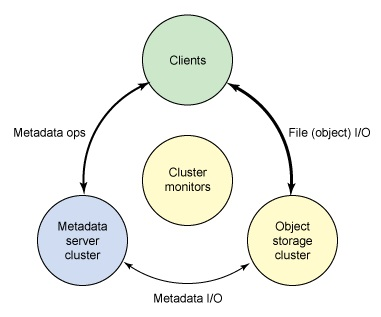
\includegraphics[scale=0.90]{imagens/arquiteturaCeph1.jpg}
    \caption{Arquitetura conceitual do sistema de arquivos distribuídos Ceph} \cite[p. 2]{jones}
    \label{fig:arquiteturaceph1}
    \end{figure}
    
    Os clientes (usuário dos dados) executam operações de metadados, que são operações que localizam os dados utilizando os servidores de metadados. Por esta vez, os servidores de metadados gerenciam a localização de dados já existentes e também de novos dados. E o armazenamento dos metadados é feito no cluster de armazenamento. As funções POSIX como abrir, fechar e renomear, são gerenciadas através dos servidores de metadados, devido aos arquivos de I/O ocorrerem entre o cliente e o \textit{cluster} de armazenamento de objetos. Já as funções POSIX como ler e renomear são gerenciadas diretamente no cluster de armazenamento de objetos \cite{jones}. 
    
\subsubsection{Arquitetura em camadas}
\label{subsec:arqcamadas}

    Conforme a Figura \ref{fig:arquiteturaceph2}, pode-se dividir o Ceph em 3 camadas: interface do cliente (Ceph \textit{client interface}), servidores de metadados (\textit{metadata servers}) e sistema de armazenamento distribuído.
    
    \begin{figure}[htb]
    \centering
    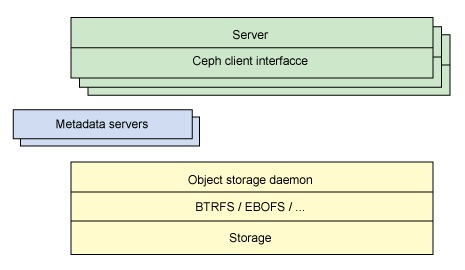
\includegraphics[scale=0.90]{imagens/arquiteturaCeph2.jpg}
    \caption{Arquitetura em camadas do sistema de arquivos distribuídos Ceph} \cite[p. 3]{jones}
    \label{fig:arquiteturaceph2}
    \end{figure}
    
    Na camada de interface, um conjunto de servidores acessa o sistema Ceph através da interface do cliente. Este acesso compreende o relacionamento entre servidores de metadados e armazenamento no nível do objeto. Já na camada de armazenamento distribuído, são projetados o gerenciamento de replicação de dados, a detecção de falhas, a recuperação e a subsequente migração de dados.
    

\subsubsection{Funcionamento}
    A Figura \ref{fig:sistemaceph} exibe a interação dos módulos do projeto Ceph, citados nas arquiteturas \ref{subsec:arqconceitual} e \ref{subsec:arqcamadas}, onde o cliente é o usuário do sistema de arquivos distribuído, o \textit{Ceph metadata daemon} (cmds) fornece os serviços de metadados, o \textit{Ceph object storage daemon} (cosd) fornece o armazenamento real e o \textit{Ceph monitor} (cmon) fornece o gerenciamento de \textit{cluster}. 

    \begin{figure}[htb]
    \centering
    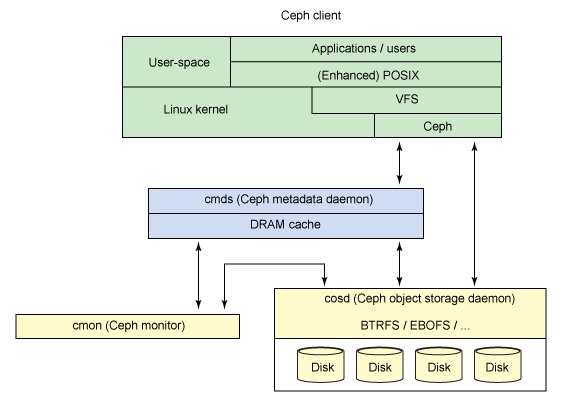
\includegraphics[scale=0.90]{imagens/sistemaCeph.jpg}
    \caption{Funcionamento Sistema Ceph} \cite[p. 4]{jones}
    \label{fig:sistemaceph}
    \end{figure}

Após se conhecer as arquiteturas e a interação entre elas, pode-se destacar as seguintes funcionalidades do Ceph:
\begin{itemize}
 \item Inteligência distribuída:  simplicidade na interface do cliente e capacidade de escalabilidade, mesmo que dinamicamente. Isto se deve ao fato do sistema de arquivos Ceph possuir inteligência distribuída nos nós e não concentrada em um só servidor.
 \item Sistema adaptável: o gerenciamento do espaço de nomes do sistema de arquivos é tarefa do servidor de metadados (cmds). Apesar do armazenamento dos dados ser feito no \textit{cluster} de armazenamento de objetos, o gerenciamento destes é feito separadamente para suportar a escalabilidade. Com isso, o servidor de metadados consegue, de maneira adaptável, replicar e distribuir o espaço de acesso para evitar pontos de acesso.
 \item Tolerância a falhas: quando dispositivos de armazenamento de objetos falham ou novos objetos são adicionados, monitores detectam e mantêm um mapa de cluster válido mesmo que de modo distribuído. 
 \end{itemize}


 
\subsection{GlusterFS}
\label{sec:gluster}

GlusterFS é um sistema de arquivos distribuídos e descentralizado, de código aberto, com escalabilidade a nível de petabytes e com conexões de milhares de clientes, criado recentemente e ainda em desenvolvimento pela empresa Z Research. É um sistema de arquivos com um \textit{design} modular, empilhável e sua arquitetura eliminou a localização de metadados através da utilização do algoritmo de hash elástico (\textit{Hashing Algorithm Elastic} \footnote{O algoritmo de hash elástico é utilizado para localizar dados no conjunto de armazenamento, remover gargalos de I/O e eliminiar pontos de falha. O acesso aos dados é totalmente paralelizado e o desempenho é linearmente escalável.}). Tal arquitetura garante melhor desempenho, escalabilidade linear e confiabilidade. O objetivo principal deste sistema é a escalabilidade, sendo que para isso seus projetistas utilizaram conceitos da computação de alto desempenho, como a agregação. Sobre ele, pode-se executar diversos sistemas operacionais, como Linux, FreeBSD, OpenSolaris e Mac OS X \cite{Mohanty2014} .

Basicamente, GlusterFS agrega múltiplas unidades de armazenamento remotas em um único volume. As unidades de armazenamento, chamadas \textit{bricks}, são distribuídas pela rede em um único sistema de arquivos paralelo, permitindo uma escalabilidade de milhares de \textit{bricks} e vários petabytes de armazenamento. Os clientes, que também podem ser simultaneamente servidores de dados, montam os diretórios compartilhados pelos servidores, tendo assim acesso a uma parte ou a todo o conteúdo compartilhado.

A maior parte das funcionalidades no GlusterFS são implementadas através de tradutores, que são objetos binários compartilhados, carregados em tempo de execução. Esses objetos possuem interfaces de comunicação estritamente definidas, de modo que os mesmos podem ser carregados tanto pelos clientes como pelos servidores. O conceito de tradutores foi herdado do sistema operacional GNU Hurd. Novos tradutores podem ser escritos através de uma interface definida pelo GlusterFS. Toda a implementação do sistema é feita no espaço de usuário do sistema operacional, através do módulo Fuse (\textit{Filesystem in Userspace}). Isso proporciona maior flexibilidade ao administrador, que não precisa ter privilégios especiais para carregar o sistema. Porém, o desempenho pode ser afetado, uma vez que se faz necessário um elevado número de cópias da memória do espaço de usuário para o espaço do núcleo do sistema operacional.

Os servidores GlusterFS são compatíveis com POSIX, desta forma, é possível utilizar qualquer sistema de arquivos \textit{ondisk} que suporta atributos estendidos (ext4, XFS, entre outros) para formatar e para armazenar dados em discos. O acesso aos dados pode ser feito utilizando protocolos de acesso padrão da indústria, como \textit{Network File System} (NFS) e \textit{Servidor Message Block} (SMB).

O sistema GlusterFS consiste em vários nós interligados, formando um \textit{cluster} para organizar e manipular grandes quantidades de arquivos e permitir que aplicações consigam utilizar este recurso. Conforme a Figura \ref{fig:glusterArq}, o modelo de comunicação utilizado por este sistema de arquivos é o Mestre/Escravo.

    \begin{figure}[htb]
    \centering
    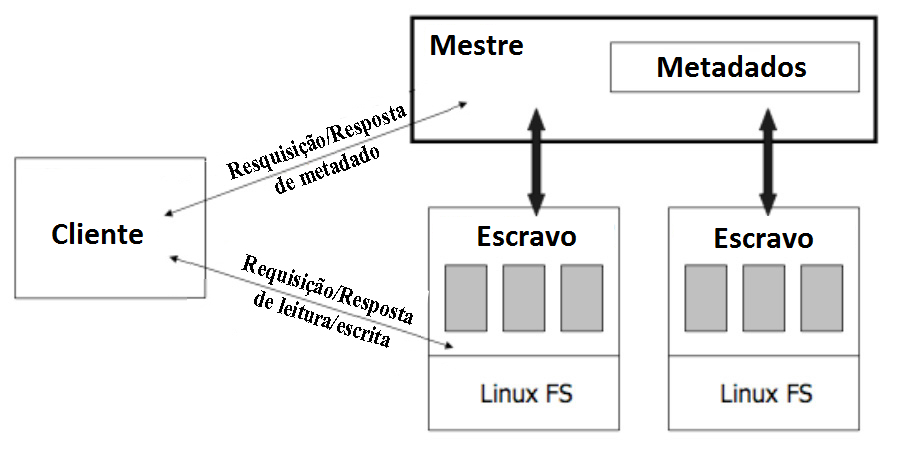
\includegraphics[scale=0.50]{imagens/GlusterFSArq.png}
    \caption{Arquitetura do GlusterFS} \cite{Roman2012}
    \label{fig:glusterArq}
    \end{figure}    

O Mestre é o responsável por coordenar o \textit{cluster}. Ele informa ao cliente a localização de cada fragmento que compõe o arquivo. Tais fragmentos ficam armazenados nos Escravos e possuem tamanho de 64 MB. 


\section{Gerenciador de \textit{Guests}}

Existem várias ferramentas de virtualização como: Virtualbox, VMWare, Xen, Virt-Manager, entre outras. O Virt-Manager foi escolhido como objeto de estudo por ser \textit{Open Source} e por possuir o KVM como módulo de virtualização, o qual já está incluído nas distribuições Linux.

\subsection{Virt-Manager}

Virt-Manager é uma interface gráfica que possui diversos software em camadas abaixo da interface gráfica, que são responsáveis pela flexibilidade do Virt-Manager \cite{PabloHess}.

    A primeira camada é composta pelo libvirt, uma API que oferece uma forma unificada de executar ações em múltiplas plataformas de virtualização, o qual suporta as seguintes plataformas: KVM, QEMU, Xen, VirtualBox, VMware, entre outras \cite{libvirt}.

    A segunda camada tratará sobre o KVM (\textit{Kernel-based Virtual Machine}).
    
    \subsection{KVM}
   KVM é um módulo que provê a pilha de software necessária para virtualização \cite{kvm}. Ele é um software de código aberto que permite a criação de \textit{guests} e também é visto como um subsistema do Linux, uma vez que seu componente de \textit{kernel} está incluído nas distribuições Linux (a partir da versão 2.6.20). Quando utilizado com QEMU (Quick EMUlator) permite a criação de uma \textit{guest} que executa com baixo \textit{overhead} (sistema criado na \textit{guest} funciona semelhante ao que roda na máquina física) \cite{KVM2}.
    As principais características do KVM são: gerenciamento de \textit{guests} com segurança, substituição de várias máquinas físicas por um servidor virtual, auxiliando assim o desenvolvimento de novos sistemas.

    
    \begin{figure}[htb]
    \centering
    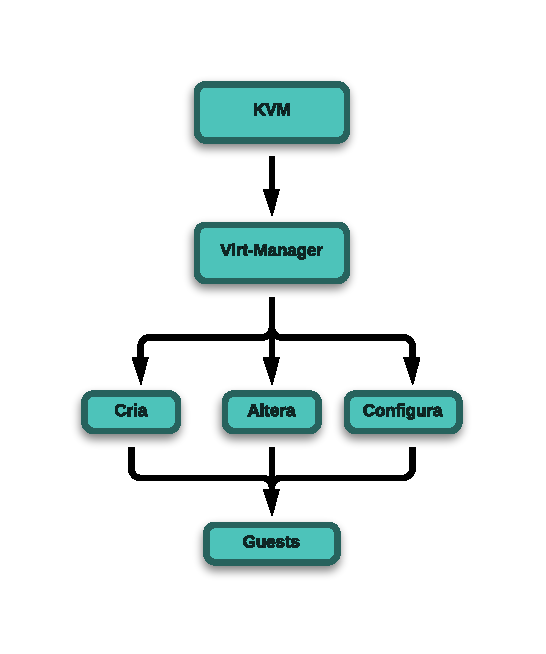
\includegraphics[scale=0.80]{imagens/kvm.pdf}
    \caption{Diagrama KVM x \textit{Virt-Manager}}
    \label{fig:kvm}
    \end{figure} 
    
    A Figura \ref{fig:kvm} exibe o diagrama \textit{botton-up} do sistema de gerenciamento de \textit{guests}. O sistema de virtualização do KVM conta com um sistema de gerenciamento chamado de Virt-manager, que provê um ambiente gráfico através do qual se pode criar, configurar e alterar os parâmetros da máquina virtual, incluindo os recursos de memória, configurações de rede e disco \cite{KVM2}.


\section{Balanceamento de Carga}

    O balanceamento de carga é um método utilizado para a distribuição de cargas de trabalho entre recursos de computação, tais como computadores, \textit{cluster} de computadores, ligações de rede, unidades de processamento central ou unidades de disco. O balanceamento de carga tem como objetivo otimizar a utilização de recursos, maximizar a produção, minimizar o tempo de resposta e evitar a sobrecarga de qualquer um dos recursos. Utilizando múltiplos componentes com o balanceamento de carga, em vez de um único componente pode-se aumentar a confiabilidade através da redundância. O balanceamento de carga é normalmente fornecido pelo software ou hardware dedicado, como um switch multicamada ou um processo do servidor DNS.

    O balanceamento consiste principalmente em reencaminhar o tráfego por caminhos alternativos a fim de descongestionar os servidores mais sobrecarregados.

\subsection{Nginx}

O Nginx é um servidor web com balanceamento de carga escrito por Igor Sysoev. O projeto surgiu em 2002 para atender as necessidades de um site russo com alto tráfego, cerca de 500 milhões de requisições por dia. Hoje o sistema é utilizado por diversos sites, tais como: SourceForge e Hulu.com. Ele trabalha com grande volume de requisições HTTP e torna as aplicações web mais ágeis, escaláveis, rápidas e seguras \cite{nginx}.

Dentre as principais características deste servidor web, estão:

\begin{itemize}
\item Velocidade: o servidor Nginx faz o uso de soquetes assíncronos. Um processo por núcleo é o suficiente para atender milhares de conexões, diminuindo a carga da CPU e o consumo de memória.
\item Facilidade de uso: suas configurações são mais simples de serem ajustadas que outros servidores web, como Apache. Em poucas linhas é possível configurar o servidor. 
\item Modularidade:  Nginx além de possuir código aberto, possui diversos \textit{plug-in} que atuam como módulos para as mais variadas funcionalidades.
\end{itemize}



A Figura \ref{fig:nginx}, exibe a arquitetura modular do Nginx. Ele é composto por núcleo e módulos funcionais. O núcleo é responsável por manter a conexão entre os diferentes módulos nas diferentes etapas de processamento, funcionamento este conhecido como Mestre/Escravo. A arquitetura modular permite aos desenvolvedores estender o conjunto de recursos do servidor web sem modificar o núcleo, sendo esta uma das principais vantagens do Nginx.

    \begin{figure}[htb]
    \centering
    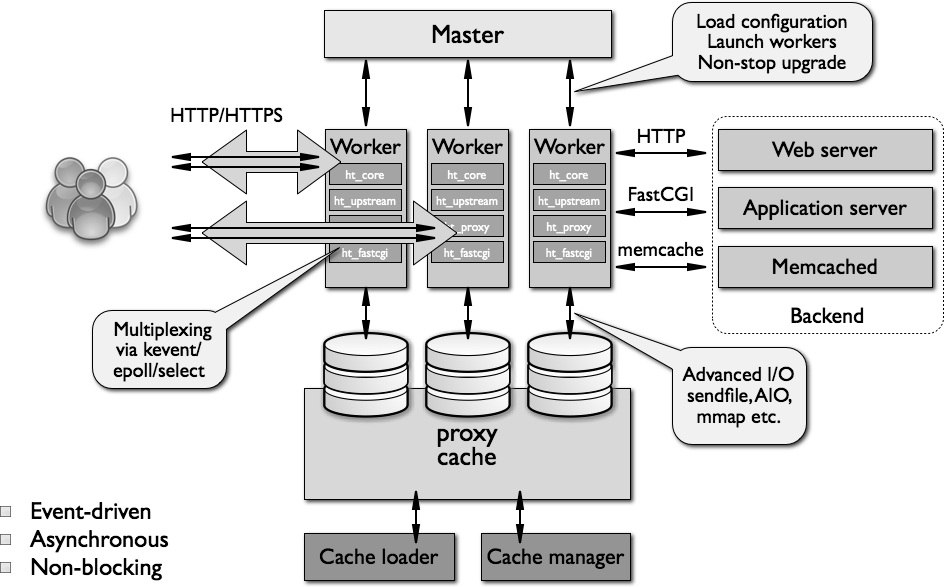
\includegraphics[scale=0.40]{imagens/nginx.png}
    \caption{Arquitetura do Nginx} \cite{nginx}
    \label{fig:nginx}
    \end{figure} 

O Nginx é comumente instalado entre a rede e a aplicação para gerenciar o processamento de concorrência, o endereçamento de URL, o balanceamento de carga HTTP, terminação SSL, cache e políticas de segurança. O serviço de balanceamento de carga e cache de conteúdo visam oferecer uma plataforma rentável e altamente disponível para os aplicativos hospedados. O balanceamento de carga é feito a partir das requisições recebidas pelo \textit{frontend} e distribuidas entre os \textit{backends} (servidores de aplicativos). Ele fornece balanceamento de dois níveis com base em cookies. O primeiro é à uma taxa de um nó. E o segundo é à velocidade de um grupo de nós interligados por uma mesma sessão \cite{Jelastic2014}.


\subsection{HAProxy}

O HAProxy é um balanceador de carga de alto desempenho para HTTP e TCP. Ele recebe as conexões dos usuários e atua como um \textit{proxy}, criando um canal entre o usuário e um dos servidores de aplicação. De acordo com \textit{benchmarks} elaborados pelo desenvolvedor, a ferramenta possui desempenho de mais de 40 mil conexões por segundo utilizando rede de 10 Gbps \cite{HAProxy2009}.

Esta aplicação possui alguns mecanismos para escolher o servidor web que deve encaminhar a solicitação ao usuário. Dentre as estratégias de escalonamento suportadas, estão:

\begin{itemize}
\item \textit{Round-robin}: o servidor é escolhido de forma circular, independente da carga em cada um dos servidores de aplicação;
\item Menos conexões: o servidor com menos conexões é escolhido, o que garante que o servidor mais ocioso seja utilizado;
\item Cookie: o HAProxy tentará sempre indicar o mesmo servidor que o usuário conectou pela primeira vez e
\item Hash de IP: neste caso a aplicação irá escolher o servidor de acordo com o IP.
\end{itemize}

\section{Kickstart - Fedora}

Kickstart é um sistema utilizado para automatizar processos de instalações, parcialmente ou em sua totalidade. Os arquivos são configurados para conter as respostas para as perguntas feitas pelos programas de instalação, tais como fuso horário, unidade que deve ser particionada, nome do sistema, nome dos usuários, quais pacotes devem ser instalados, entre outras. Os arquivos Kickstart geralmente são utilizados para implantar o SO em um grande número de máquinas de uma só vez, sem que haja intervenção humana no processo \cite{Fedora}.

\subsection{Utilizando o Kickstart}

As instalações Kickstart podem ser realizadas utilizando um DVD local, um disco rígido local, ou através do NFS, FTP, HTTP, ou HTTPS.

Para utilizar o Kickstart deve-se:
\begin{itemize}
\item criar um arquivo Kickstart;
\item criar uma mídia de inicialização ou configurar um servidor de inicialização de rede (PXE);
\item disponibilizar o arquivo Kickstart em uma mídia removível, ou em uma unidade de disco rígido, ou em um local de rede e
\item na opções de \textit{boot}, informar ao instalador onde encontrar o arquivo Kickstart.
\end{itemize}




    \begin{figure}[htb]
    \centering
    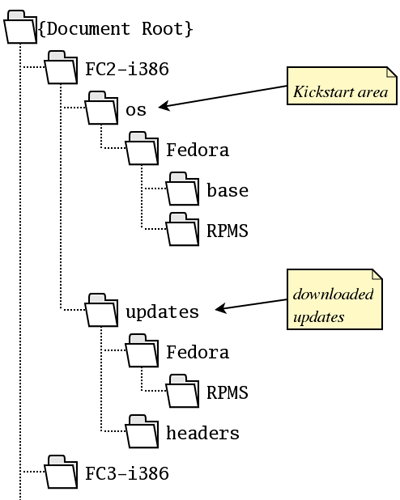
\includegraphics[scale=0.60]{imagens/kickstart.png}
    \caption{Estrutura de um diretório de repositório \textit{yum}, hospedado em servidor KickStart} \cite{McCallum2005}
    \label{fig:kickstartdir}
    \end{figure} 





\section{JMeter}

O JMeter é uma ferramenta \textit{desktop} para testes de desempenho, desenvolvida utilizando a linguagem Java e licenciada sob os termos da Licença Apache, versão 2.0. Esta ferramenta foi primeiramente utilizada para realizar testes em aplicações web, mas tem expandido suas funcionalidades, podendo realizar testes funcionais em bancos de dados \cite{De2013}.

Como o JMeter é totalmente desenvolvido em Java, é possível operá-lo em qualquer sistema operacional que possua Java instalado.

\subsection{CassJMeter}
\label{sec:cassjmeter}

O CassJMeter é um \textit{plugin} que foi desenvolvido pela Netflix para realizar testes de carga em banco de dados Cassandra. Ele funciona como um cliente de Cassandra e pode enviar requisições utilizando as interfaces Astyanax ou Thrift \cite{DenisSheahan2012}.

De acordo com o estudo de caso realizado pela Netflix, usando 60 instâncias adicionais como clientes e executando o programa de estresse (CassJMeter) conseguiu-se atender a uma carga de trabalho de 1,1 milhões de clientes escrevendo por segundo. Os dados foram automaticamente replicadas em três zonas, perfazendo um total de 3,3 milhões de gravações por segundo em todo o \textit{cluster} \cite{Crockcroft2011}. 
Para medir a escalabilidade, o mesmo teste foi executado com 48, 96, 144 e 288 casos, com respectivamente 10, 20, 30 e 60 clientes. A carga sobre cada instância foi muito semelhante em todos os casos, conforme mostra a Figura \ref{fig:benchNetflix}.

    \begin{figure}[htb]
    \centering
    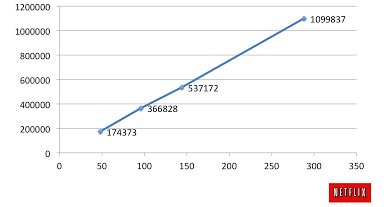
\includegraphics[scale=0.7]{imagens/scale.png}
    \caption{Escalabilidade linear do \textit{cluster} Cassandra com fator de replicação 3} \cite{Crockcroft2011}
    \label{fig:benchNetflix}
    \end{figure} 

\section{Base de dados (Cassandra)}

O Cassandra é um sistema de banco de dados NoSQL. Ele é um banco de dados altamente escalável, capaz de gerenciar grandes volumes de dados em vários \textit{datacenters} e em nuvem. Este banco também oferece disponibilidade contínua, escalabilidade linear, modelo dinâmico de dados e tempos de respostas rápidos.

Estas e outras características, bem como o porquê da escolha desssa base de dados serão melhor estudadas no Capítulo \ref{cap:cassandra}. 

% Ambiente Experimental
\chapter{Ambiente Experimental}
\label{cap:ambExperimental}
Os diagramas presentes nesta seção, detalham as configurações do servidor onde foram feitas as análises deste trabalho. 

\section{Rack do servidor utilizado para testes dos modelos de escalabilidade}

Foi utilizado durante todo trabalho o \textit{rack} Maritaca, que utiliza o sistema operacional Ubuntu 14.04 x86/64, com kernel 3.8.0-39-generic.

Conforme a Figura \ref{fig:maritaca-rack} e \ref{fig:real}, o \textit{rack} do servidor utilizado para as modelagens deste trabalho é composto por 9 \textit{nodes}, 2 \textit{header nodes}, 4 \textit{nobreaks} que alimentam as réguas de energia (\textit{power strip}), 2 \textit{switchs}, 1 teclado, 1 mouse e 1 monitor.

    \begin{figure}[htb]
    \centering
    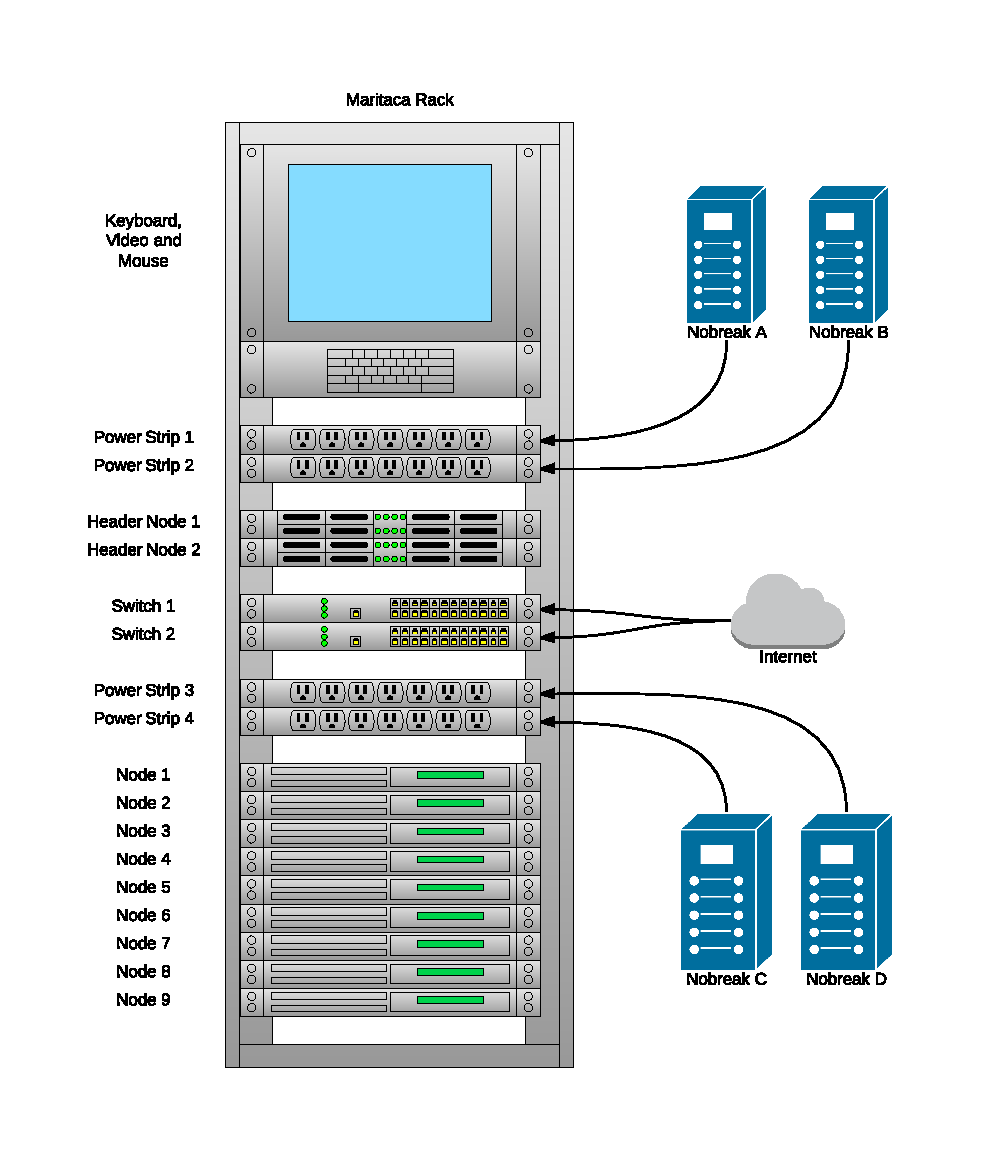
\includegraphics[scale=0.6]{imagens/maritaca-rack.pdf}
    \caption{\textit{Rack} do servidor Maritaca}
    \label{fig:maritaca-rack}
    \end{figure}

\begin{figure}[!htb]
\centering
\subfloat[Visão Frontal]{
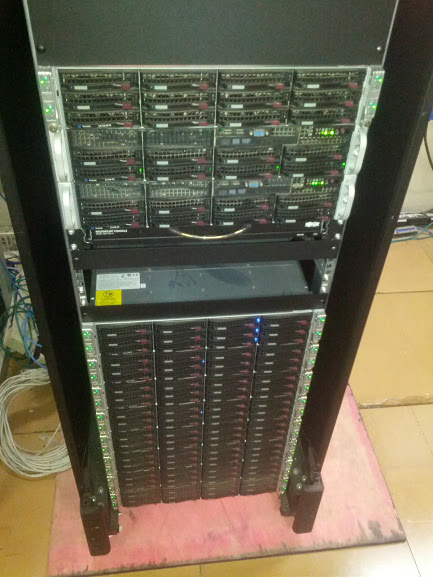
\includegraphics[height=7cm]{imagens/rack-frente.jpg}
\label{fig:frente}
}
\quad %espaco separador
\subfloat[Visão Traseira]{
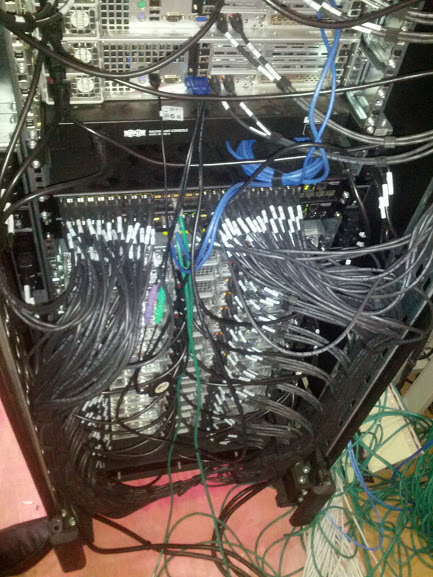
\includegraphics[height=7cm]{imagens/rack-tras.jpg}
\label{fig:tras}
}
\caption{Imagem real do \textit{rack} do servidor Maritaca}
\label{fig:real}
\end{figure}




\subsection{\textit{Nodes}}

Os \textit{nodes} possuem configurações de rede dinâmica enquanto no \textit{headnode} é estática. Apesar dos \textit{nodes} serem capazes de inicializar o sistema operacional, mesmo sem rede, o \textit{boot} nessas máquinas é controlado pelo \textit{headnode} que só permite a continuidade do \textit{boot} se toda a infraestrutura de rede necessária para virtualização e agregação remota de discos estiver satisfatória.

O \textit{rack} contém 9 \textit{nodes}, sendo que cada um possui 4 máquinas servidoras. Cada máquina destas é composta por 2 CPUs com a seguinte configuração: 

    \begin{itemize}
    
    \item Processador AMD Opteron (tm) 6344
    
        \begin{itemize}
        \item 12 \textit{cores};
        \item 200 MHz de \textit{clock};
        \item frequência de 2,6 GHz e
        \item 3 \textit{caches} com \textit{clock} de 1 GHz cada. Sendo que a primeira possui 576 kB de capacidade e as demais 12 MB.
        \end{itemize}
        
    \item 4 pentes de memória DDR3 \textit{synchronous}, sendo:
        
        \begin{itemize}
        \item 2 pentes com capacidade de 8 GB;
        \item 2 pentes com capacidade de 4 GB e
        \item ambos com 1,6 GHz de \textit{clock}.
        \end{itemize}

    \item 3 discos ATA \textit{Disk} com capacidade de 2 TB cada.

    \end{itemize}
    
    A Figura \ref{fig:node} exibe a frente de um \textit{node} e seus componentes de interface.
    
     \begin{figure}[htb]
    \centering
    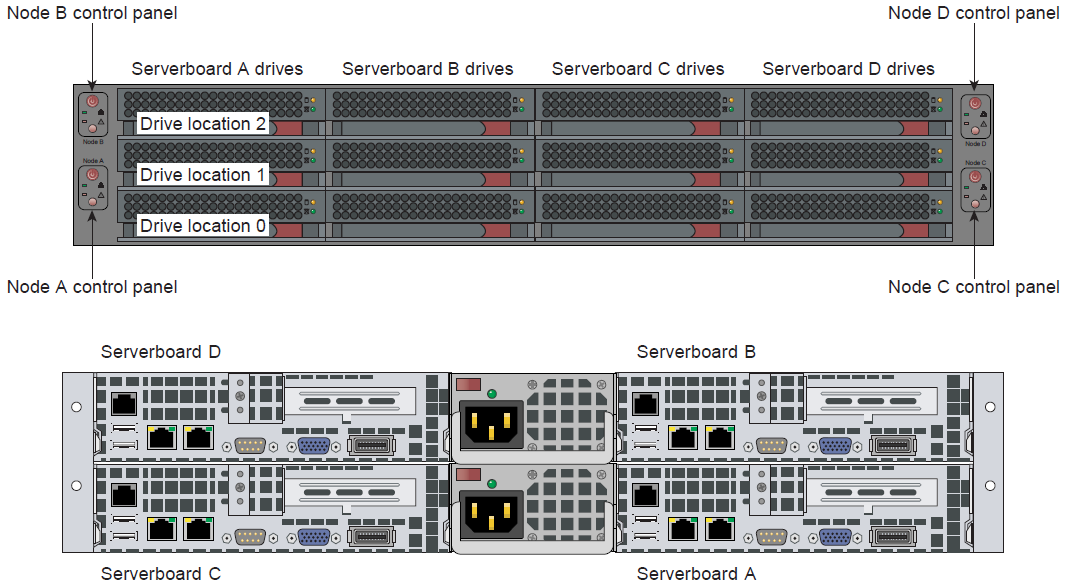
\includegraphics[scale=0.50]{imagens/node.png}
    \caption{Frente do \textit{node} e componentes de interface traseiros} \cite{SGI2011i}
    \label{fig:node}
    \end{figure}   
    
    
\subsection{\textit{Head Nodes}}

O \textit{head node} tem como função primária alojar todos os serviços necessários para o funcionamento dos \textit{nodes} que pertencem ao seu grupo principalmente as definições de rede, controle de \textit{boot} pxe, dhcp, dns interno, repositório interno para instalações automatizadas, \textit{midleware} de controle do \textit{cluster}.

    O \textit{rack} possui 2 \textit{head nodes}. Cada um possui 2 CPUs, estas por sua vez, possuem a seguinte configuração:

    \begin{itemize}
    
    \item Processador AMD Opteron (tm) 6344;
    
        \begin{itemize}
        \item 12 \textit{cores};
        \item 200 MHz de \textit{clock};
        \item frequência de 2,6 GHz e
        \item 3 \textit{caches} com \textit{clock} de 1 GHz cada. Sendo que a primeira possui 576 kB de capacidade e as demais 12 MB.
        \end{itemize}
        
    \item 4 pentes de memória DDR3 \textit{synchronous}, com capacidade de 8GB cada e 1,6 GHz de \textit{clock} em ambos;

    \item 2 discos ATA \textit{Disk} com capacidade de 2 TB cada;
    \item 1 DVD e 
    \item 2 PCI.

    \end{itemize}
    
A Figura \ref{fig:headnode} exibe a frente de um \textit{head node} e seus componentes de interface.

    \begin{figure}[htb]
    \centering
    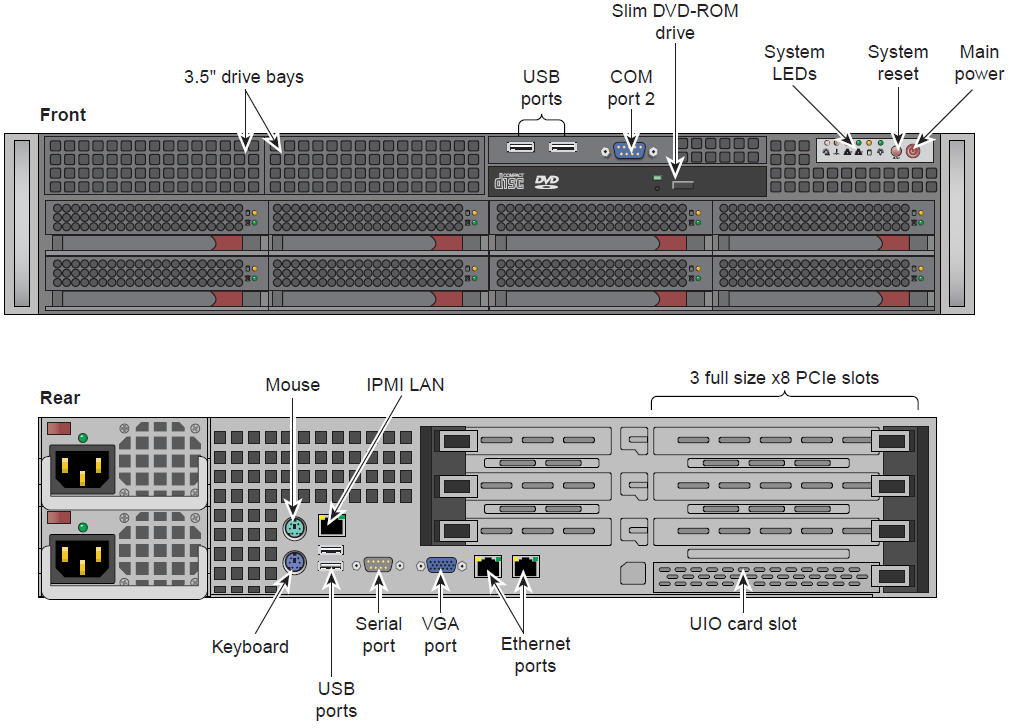
\includegraphics[scale=0.50]{imagens/headnode.png}
    \caption{Frente do \textit{head node} e componentes de interface traseiros} \cite{SGI2011}
    \label{fig:headnode}
    \end{figure}

\section{Redes virtuais e Redes Privadas}

    Em um sistema em computação em nuvem é extremamente importante isolarmos a rede dos \textit{hosts} da rede dos \textit{guests}. São redes que possuem funcionalidades diferentes e gerenciam pacotes de formas diferentes umas das outras.
    
    O isolamento de recursos garante que as redes virtuais operem de forma independente, assim, o uso de recursos de um roteador virtual não interfere no desempenho dos demais. O isolamento de recursos é importante porque evita a negação de serviços, já que uma rede virtual não consegue exaurir os recursos de outra rede virtual \cite{Carlos2011}.
    
    Na redes dos \textit{guests} são gerenciados pacotes de menores tamanhos, porém em maior quantidade. Pode-se citar como exemplo um servidor Tomcat, que responde a diversas requisições onde os pacotes possuem MTU $\leq$ 1500.
    Já na rede dos \textit{hosts}, existe outra infraestrutura de comunicação entre cada \textit{host}. Pode-se ter comunicações entre diferentes máquinas utilizando fibra óptica em placas de rede com transmissões em Gigabit.
    Neste tipo de rede, os \textit{hosts} se comunicam poucas vezes, porém os pacotes possuem MTU $\leq$ 9000, como ilustra a Figura \ref{fig:redesvirtpriv}.
    
    \begin{figure}[htb]
    \centering
    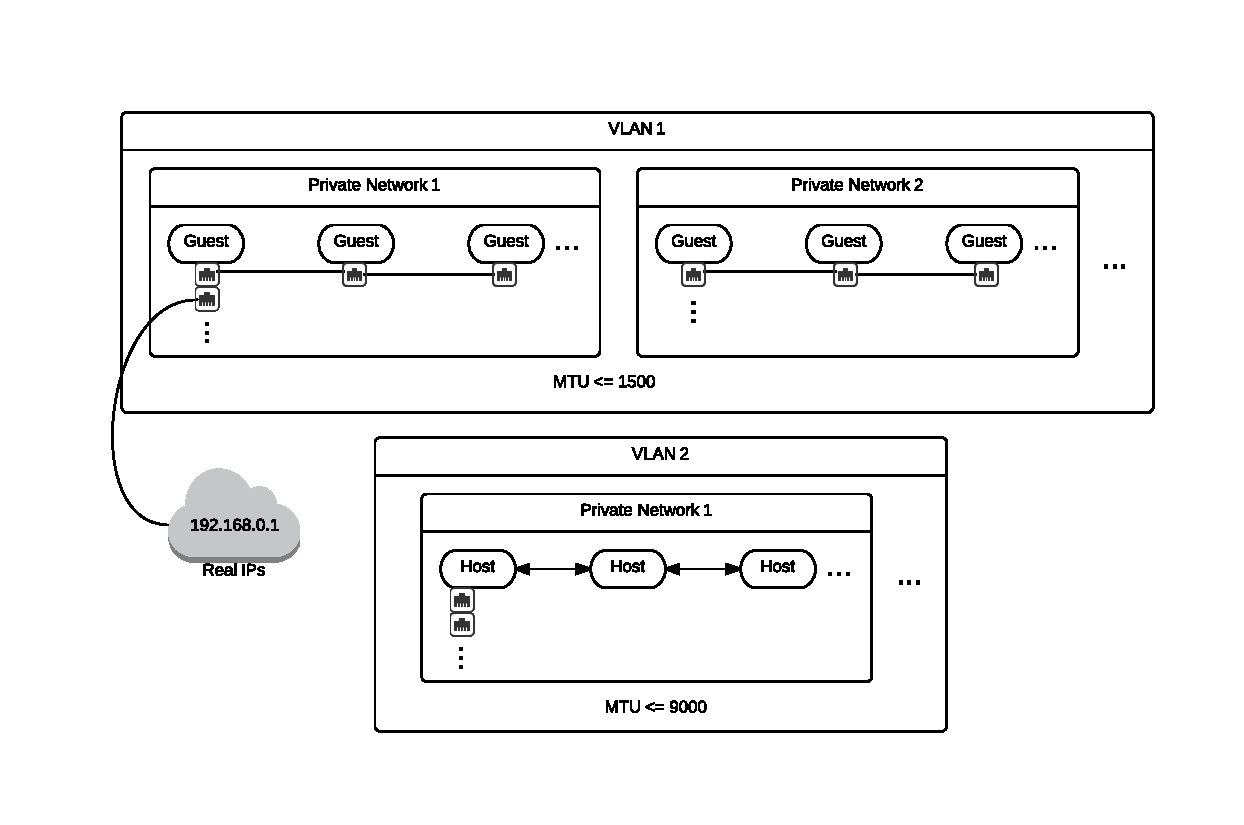
\includegraphics[scale=0.50]{imagens/esquema1.pdf}
    \caption{Diagrama das redes virtuais e redes privadas}
    \label{fig:redesvirtpriv}
    \end{figure}

\subsection{Isolamento das redes virtuais}

Como é necessário o isolamento entre as redes de \textit{hosts} e de \textit{guests}, as redes privadas dos guests são criadas dentro de uma VLAN e as redes privadas dos hosts são criadas dentro de outra VLAN.
A Figura \ref{fig:isolamento} ilustra o esquema de 2 VLANs, que podem ser descritas da seguinte forma:

    \begin{itemize}
        \item CORE: VLAN que abriga os serviços compartilhados como: DNS (\textit{private}), MySQL (\textit{cluster}), Load Balance (HAProxy), entre outros.
        \item GUESTs: VLAN que abriga as diversas redes privadas dos guests\footnote{Atualmente no servidor Maritaca, estão configuradas duas redes virtuais. A primeira é para atender os projeto Maritaca e a segunda (DIS) é destinada a atender outros projetos.}. Como cada guest é criado virtualmente, ele pode ter quantas interfaces de rede forem necessárias. As quais, por sua vez, podem ou não estar dentro de outras redes privadas pertencentes a esta ou outra VLAN.
    \end{itemize}

O \textit{Firewall} tem uma interface em cada rede, seja ela privada ou não. Ele também possui um IP real e é capaz de gerar um túnel da internet diretamente para as redes privadas. Utilizando o \textit{Firewall} também é possível criar conexões diretas entre as redes privadas. Porém, uma das principais desvantagens do seu uso para criação de conexões diretas é a utilização de NAT nestas conexões, pois NAT impossibilita o rastreio do caminho dos pacotes e aumenta o processamento dos dispositivos tradutores \cite{mattos}. 

    \begin{figure}[htb]
    \centering
    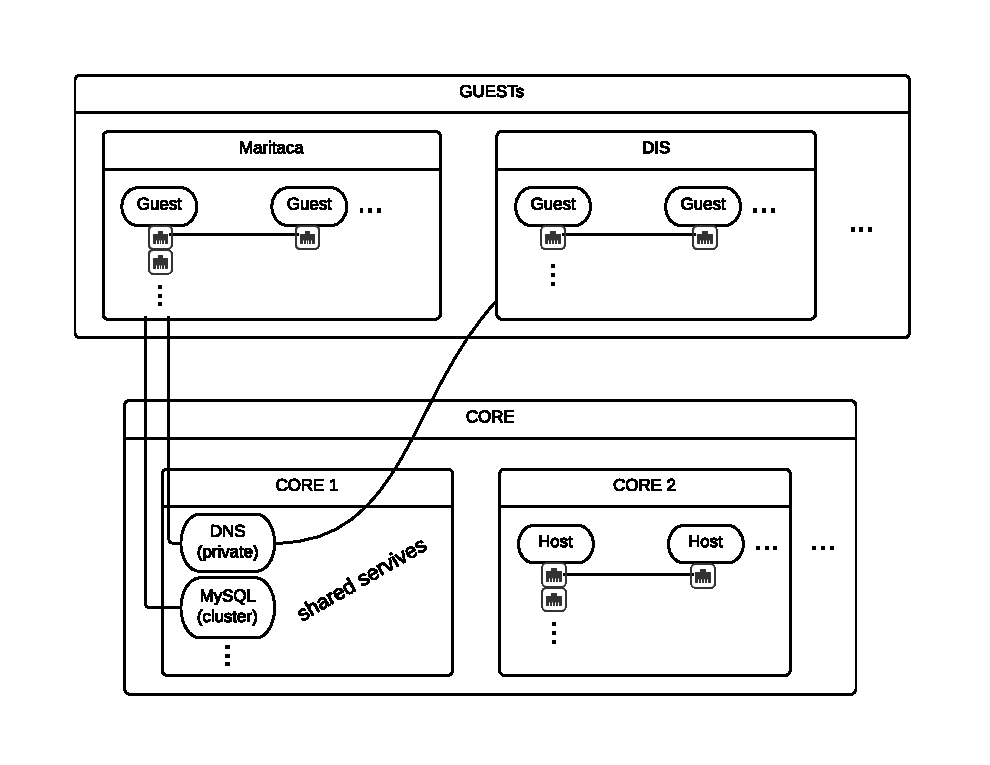
\includegraphics[scale=0.50]{imagens/esquema2.pdf}
    \caption{Isolamento das redes virtuais}
    \label{fig:isolamento}
    \end{figure}
    
\section{Balanceador de Carga (\textit{Load Balancer})}

O Balanceador de Carga recebe um pacote e direciona o mesmo ao servidor responsável pelo seu processamento.
Conforme a Figura \ref{fig:balanceador}, ele verifica a carga de cada servidor, para decidir qual servidor deverá receber aquele pacote.

    \begin{figure}[htb]
    \centering
    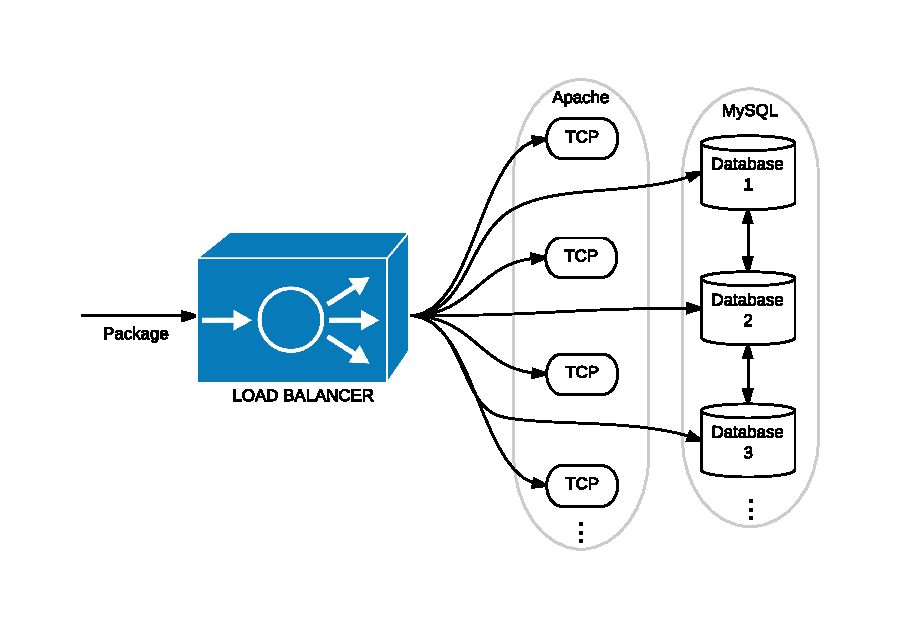
\includegraphics[scale=0.82]{imagens/esquema3.pdf}
    \caption{Esquemático do funcionamento do Balanceador de Carga}
    \label{fig:balanceador}
    \end{figure}    
    
    
\section{Integração do Balanceador de Carga às redes virtuais}
    Unindo os diagramas anteriores, temos o diagrama representado na Figura \ref{fig:integracaoloadbalan}, no qual pode-se perceber que o \textit{Load Balancer} funciona roteando pacotes para outros serviços do sistema. Além disso, o \textit{Load Balancer} pode também ser replicado de acordo com a necessidade, pois também se trata de um serviço configurado em \textit{guest}.
    
    \begin{figure}[htb]
    \centering
    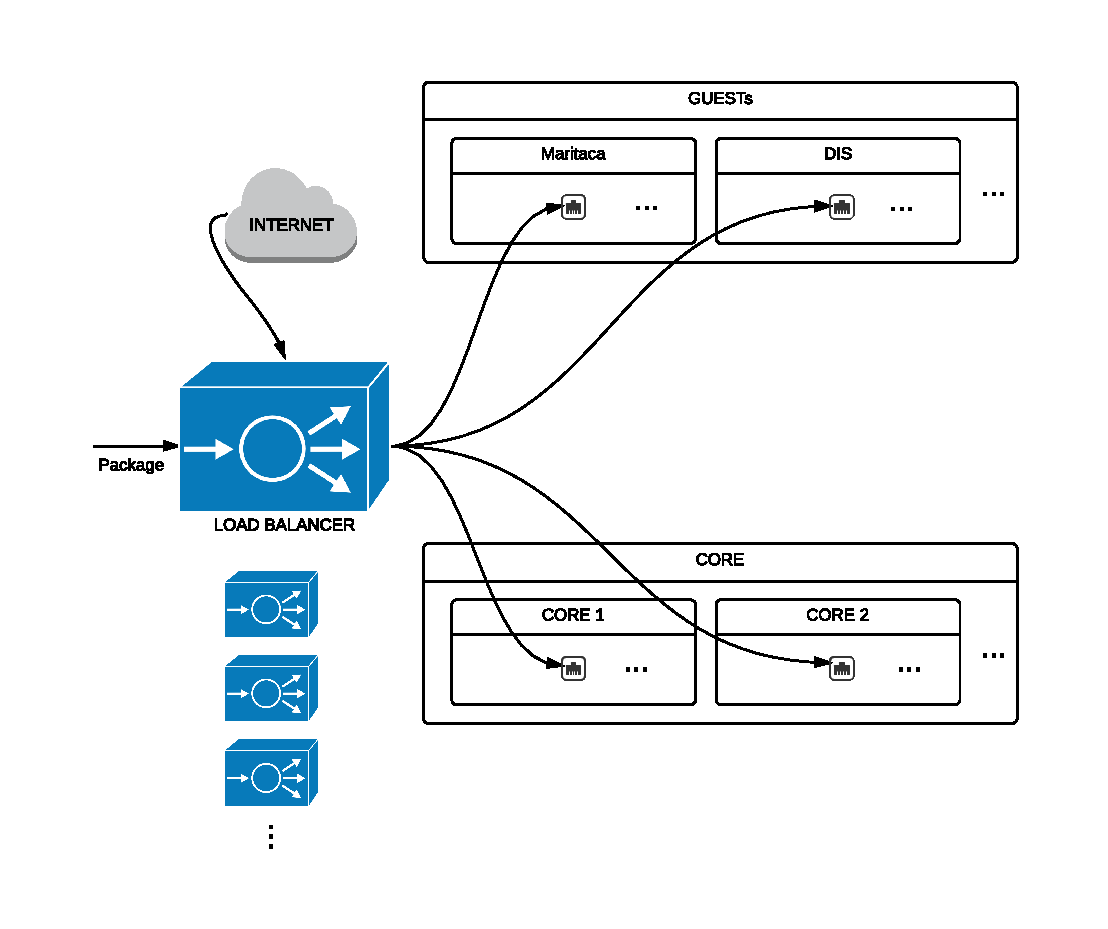
\includegraphics[scale=0.50]{imagens/esquema4.pdf}
    \caption{Integração do Balanceador de Carga às redes virtuais}
    \label{fig:integracaoloadbalan}
    \end{figure}


\section{Arquitetura do servidor}
Após a falha de um dos \textit{switches} as conexões das máquinas foram reorganizadas de forma que cada \textit{switch} atenda a um 1 \textit{headnode} e 18 \textit{nodes}. Com isso criou-se 2 grupos de máquinas denominados \textit{group1} e \textit{group2}. Esta reorganização foi necessária até que sejam adquiridos 2 cabos proprietários do fabricante do \textit{switch} capaz de conectar os \textit{switches} formando um pilha de única rede.

Os grupos de máquinas serão usados para virtualização sendo o \textit{group1} alocado para produção e \textit{group2} para testes de resiliência da infraestrutura, até que seja possível unificar os grupos. O \textit{group2} também poderá ser usado como \textit{failover} do \textit{group1} caso haja uma falha crítica de hardware, como houve com um dos \textit{switches}.

    \begin{figure}[htb]
    \centering
    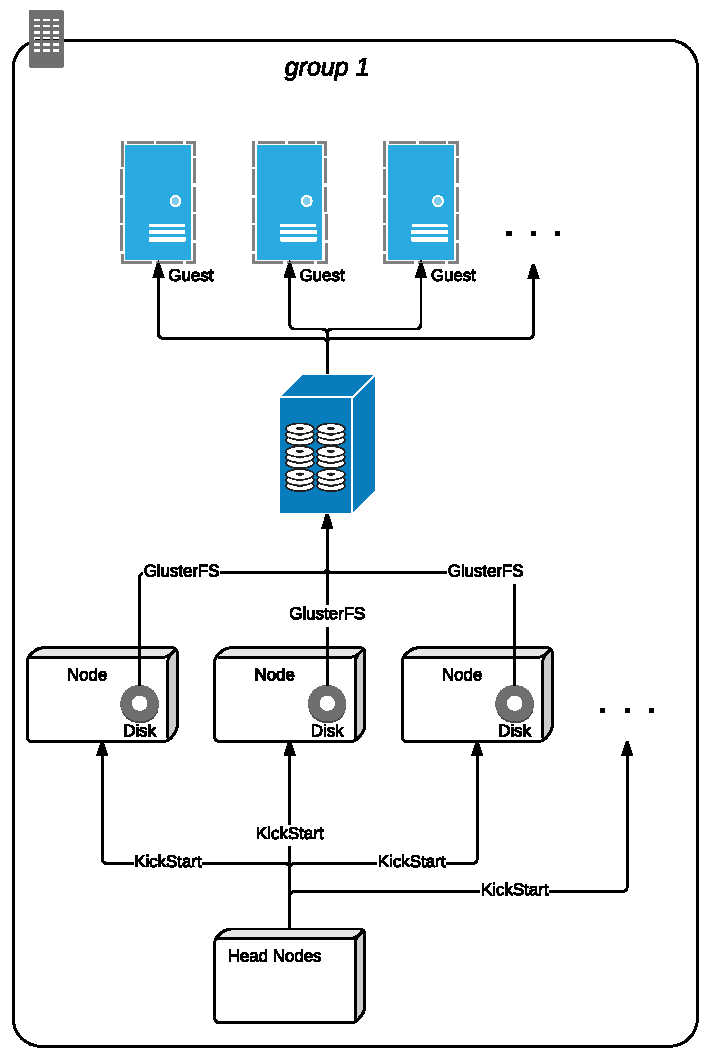
\includegraphics[scale=0.6]{imagens/group1.pdf}
    \caption{Arquitetura do \textit{group 1}}
    \label{fig:group1}
    \end{figure}

Atualmente o group1, representado na Figura \ref{fig:group1}, é composto pelo \textit{headnode}-1 e os \textit{nodes} de 32 à 20 mais o \textit{node} 18 totalizando 1 \textit{headnode} e 14 \textit{nodes}. Os 4 \textit{nodes} restantes estão alocados para o antigo grupo de trabalho do projeto Maritaca, que deverão ser incluídas no group1 assim que os serviços forem migrados para esta nova estrutura. Com 14 \textit{nodes} e 3 HDs de 2 Tb em cada foi configurado um disco virtual do tipo \textit{distributed replicated} com o glusterFS, no qual o volume replicado distribui os arquivos entre os \textit{bricks}, conforme a Figura \ref{fig:drv_gluster}. Este tipo de configuração é utilizada em servidores cuja exigência é a escala de armazenamento e a confiabilidade.  Com isso, o sistema de arquivos distribuído totaliza 38 Tb úteis para o alojamento dos discos virtuais das \textit{guests}.

    \begin{figure}[htb]
    \centering
    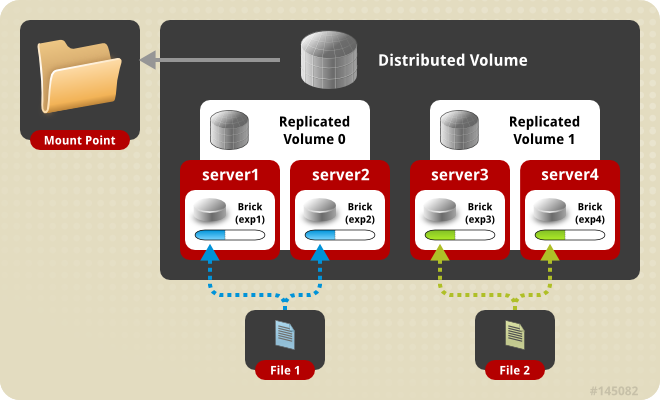
\includegraphics[scale=0.6]{imagens/Distributed_Replicated_Volume.png}
    \caption{Esquema de replicação distribuída via GlusterFS} \cite{Chandrashekar2015}
    \label{fig:drv_gluster}
    \end{figure}



Cada \textit{node} possui uma instalação Fedora Server 21 padronizada via Kickstart, sistema de arquivos distribuído via GlusterFS e camada de rede definida por software via OpenVSwitch.

Conforme a Figura \ref{fig:particoes}, a organização das partições dos \textit{nodes} pode ser vista pelo administrador executando o comando \textit{lsblk} no \textit{terminal}.

    \begin{figure}[htb]
    \centering
    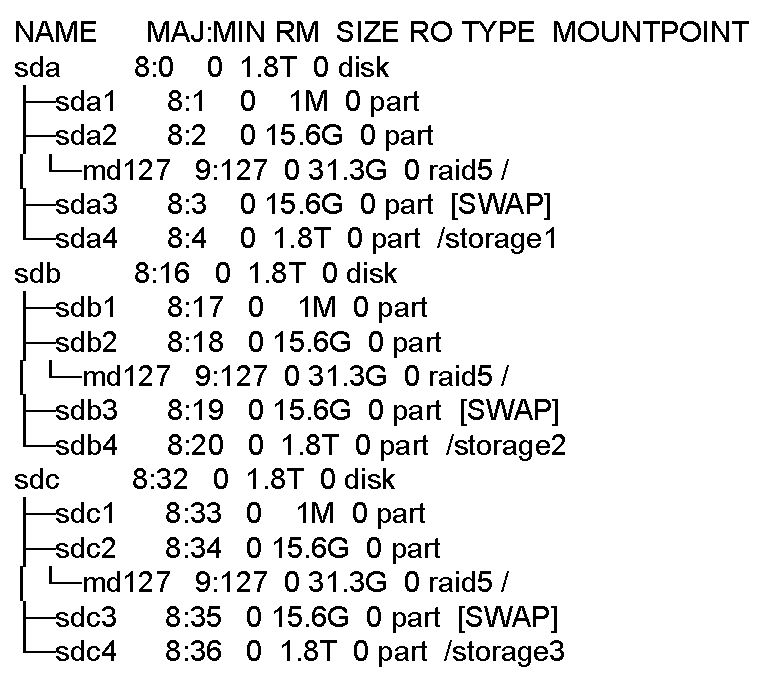
\includegraphics[scale=0.8]{imagens/particoes.pdf}
    \caption{\textit{Layout} de partições}
    \label{fig:particoes}
    \end{figure}

O \textit{layout} exibido na Figura \ref{fig:particoes}, é pré-resultado das linhas de automação, presentes no \textit{script} do Kickstart, que geram a instalação dos \textit{nodes}.
Neste \textit{layout}, o SO opera em um RAID5 que suporta a falha de um dos HDs. Os SWAPs estão distribuídos nos 3 HDs pois não são críticos para o funcionamento do sistema. A partição de \textit{boot} é replicada no ínicio de cada HD de forma que qualquer um deles contenha um setor inicializável (setor de \textit{boot}) para o RAID5 onde reside o SO. Cada HD possui uma partição de dados que será a base física para o volume GlusterFS (\textit{storage1, storage2 e storage3}). Cada \textit{storageX} é replicado via rede em outro \textit{storageX} residente em outro \textit{node} que não está na mesma lâmina. 



As \textit{guests} tem seus discos virtuais e suas configurações alojadas no volume GlusterFS. O libvirt de cada \textit{node} encarrega-se de virtualizar os recursos de CPU e memória para cada \textit{guest}. As \textit{guests} são capazes de migrar livremente entre os \textit{nodes} do group1 sem serem desligadas (\textit{livemigration}). A camada de rede necessária ao funcionamento das \textit{guests} é encapsulada na própria \textit{guest} na forma de uma abstração da camada de rede das \textit{hosts} definida e gerenciada pelo openVSwitch. A ligação entre as interfaces virtuais de rede das \textit{guests} com a rede física é feita através de VETH PAIRS ligadas às BRIDGES do openVSwitch. Estas conexões correm de forma virtualizada no kernel do SO dentro de NAMESPACES.

Conforme descrito na seção \ref{sec:gluster} o sistema de arquivos distribuídos GlusterFS agrega múltiplas unidades de armazenamento remotas em um único volume. As unidades de armazenamento (\textit{bricks}), são distribuídas pela rede em um único sistema de arquivos paralelo, permitindo uma escalabilidade de milhares de \textit{bricks} e vários petabytes de armazenamento. A Figura \ref{fig:vmfs} exibe os 42 \textit{bricks} que compõe o GlusterFS configurado no servidor Maritaca. 
    \begin{figure}[htb]
    \centering
    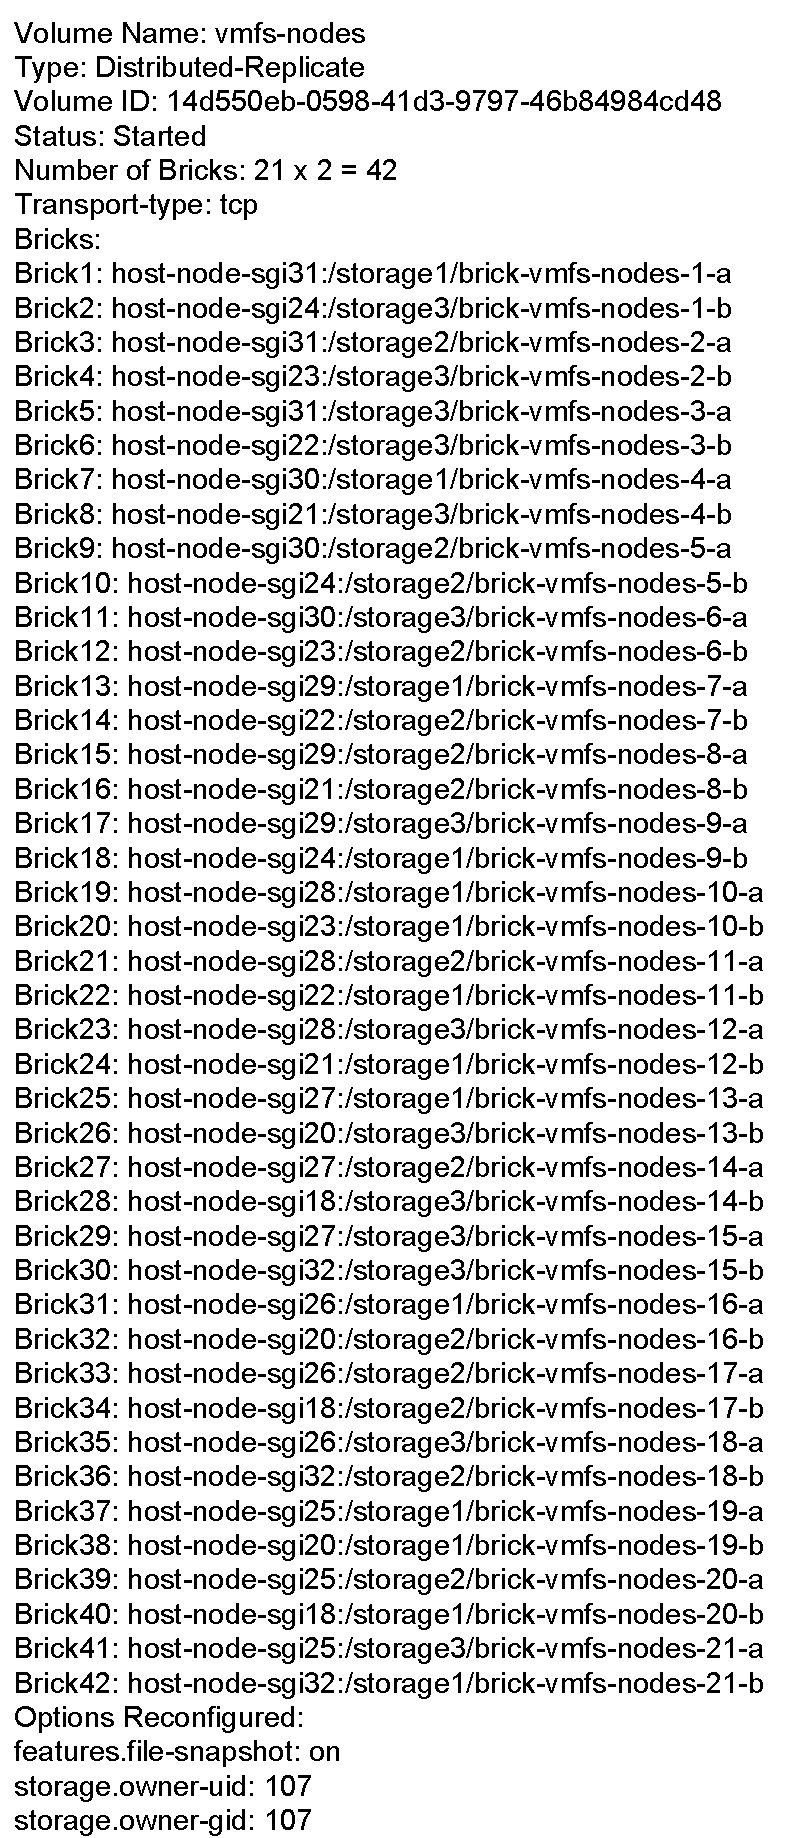
\includegraphics[scale=0.7]{imagens/vmfsnodes.pdf}
    \caption{\textit{Bricks} (GlusterFS)}
    \label{fig:vmfs}
    \end{figure}


% Banco de Dados Distribuído
\chapter{Cassandra operando em \textit{cluster}}
\label{cap:cassandra}
Este capítulo descreve a definição do banco de dados Cassandra operando em \textit{cluster}, assim como características, funcionalidades o porquê da sua escolha e como realizar avaliações neste banco. 

Cassandra é um sistema de banco de dados baseado na abordagem NoSQL (\textit{Not only Structure Query Language}), do tipo chave/valor. Nesse tipo de banco de dados, os dados são identificados através de uma chave \cite{Silva}.
A principal promessa do Cassandra é de prover um sistema de armazenamento distribuído, altamente escalável e eventualmente consistente. Para garantir essas promessas,
foram unidas características de dois sistemas NoSQL, o BigTable do Google e o Dynamo da Amazon.
Esse sistema foi criado no Facebook em 2008, por Avinash Lakshman e Prashant Malik e foi bastante usado pelo próprio Facebook para tornar a busca de mensagens mais robusta. 


Um sistema de banco de dados somente pode abranger dois itens entre consistência, disponibilidade e tolerância a partições. Entre essas três
opções, o Cassandra garante disponibilidade dos dados e tolerância a partições \cite{Silva}.

Para garantir que um grande volume de dados seja tratado de forma rápida e eficiente, o Cassandra possui por trás uma arquitetura bastante robusta e complexa. Essa arquitetura é composta por diversos sistemas distribuídos que garantem que cada parte do sistema funcione corretamente.

Quando uma requisição de leitura ou escrita é feita, qualquer nó do \textit{cluster} pode tratá-la. Através da chave, o nó que atendeu a requisição consegue saber quais nós possuem informações dos dados. O sistema então aguarda até que um número configurado de réplicas, chamado \textit{quorum}, responder com o dado, no caso de leitura; ou responder com uma confirmação, no caso de uma escrita.

\section{Particionamento de Dados}
O \textit{cluster} do Cassandra é organizado em um anel, sendo que cada nó do anel possui um intervalo de valores determinado. Os dados são divididos entre os diversos nós através de um \textit{hashing} da chave identificadora desses dados. Esse \textit{hash} gera um valor que então determina, através do intervalo de cada nó do anel, qual dessas máquinas será responsável por esse dado. Essas máquinas responsáveis pelos dados são chamadas de coordenadoras.
Essa divisão dos nós em anel facilita a adição e remoção de nós no \textit{cluster}. Quando um nó é adicionado ou removido no \textit{cluster}, somente os vizinhos desse nó são afetados. Isso garante que o sistema seja bastante escalável, já que a adição de um nó no \textit{cluster} não afeta o funcionamento de todo o sistema.

\section{Replicação de Dados}
A replicação no Cassandra é utilizada para garantir a alta disponibilidade dos dados. Cada dado é encontrado em N nós do \textit{cluster}, sendo que N é um fator de replicação configurável. O coordenador do nó (definido anteriormente) é o responsável por replicar os dados entre os N-1 nós. Essa réplica feita pelo coordenador pode ser feita de três formas diferentes: \textit{Rack Unaware}, \textit{Rack Aware} e \textit{Datacenter Aware}. No modo \textit{Rack Unaware}, o coordenador simplesmente seleciona os próximos N-1 nós do anel. Nos modos \textit{Rack Aware} e \textit{Datacenter Aware}, é utilizado um sistema externo que elege um líder, que tem como função avisar cada nó que se conecta ao \textit{cluster} a faixa de valores do anel que ele será uma réplica. A Figura \ref{fig:gravacaoCassandra} tem uma representação desse anel, onde cada nó é responsável por armazenar dados cuja chave primária esta dentro de uma faixa de valor. Essa chave primária determina em qual nó os dados serão escritos e é utilizando ela que o sistema faz cópia dos dados e os distribui entre um grupo de nós. 

    \begin{figure}[htb]
    \centering
    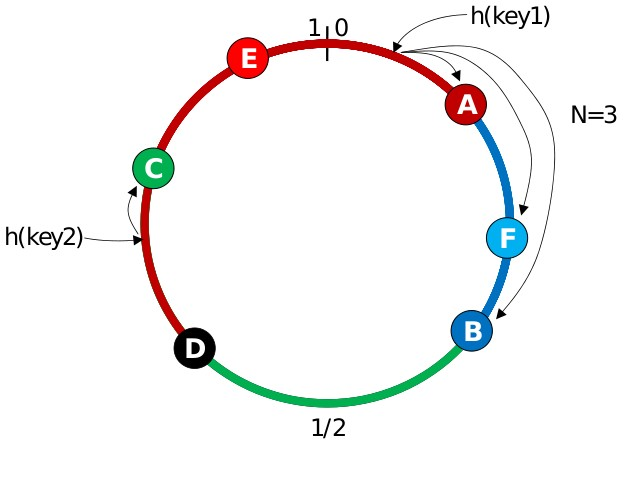
\includegraphics[scale=0.5]{imagens/cassandra.png}
    \caption{Exemplo de gravação de dados no Cassandra} \cite[p. 3]{Silva}
    \label{fig:gravacaoCassandra}
    \end{figure}
    
    
\section{Cassandra: o porquê de sua escolha}

A criação de um \textit{cluster} Cassandra é fácil de ser configurada e ampliada, os dados podem ficar distribuídos de acordo com o planejamento de utilização. Além disso, sua arquitetura é escalável e dependendo da demanda é possível aumentar o número de nós do \textit{cluster}, sem que haja interrupção do serviço.

O Cassandra também conta com menor concorrência, ou seja, o(s) \textit{webservice(s)} não acessam um único nó, ele(s) podem acessar qualquer nó a qualquer momento, fazendo com o que o sistema como um todo tenha melhor desempenho e aumento da disponibilidade.


\section{Avaliação do Cassandra}

Utilizou-se o JMeter e o CassJMeter para testar os diferentes cenários propostos para o Cassandra no projeto Maritaca \cite{DenisSheahan2012}.

\subsection{Criando um Plano de Teste}

Plano de teste é o componente básico para a criação de qualquer \textit{script} (.jmx) utilizando o JMeter e descreve uma série de passos que a ferramenta irá executar quando executar os testes \cite{De2013}. Ao plano de teste são adicionados os demais componentes pertinentes aos testes que serão executados. Os principais componentes estão ilustrados na Figura \ref{fig:plantest} e são:

\begin{itemize}
\item Thread (\textit{users}) - Grupo de usuários: representação de um grupo de usuário executando determinada(s) solicitação(ões);
\item Elemento de configuração: representação dos itens de configuração, que pode ser Cassandra \textit{Properties}, \textit{Schema Properties}, Configuração dos dados CSV, entre outros;
\item Testador: representação de uma solicitação, que pode ser HTTP, FTP, Cassandra \textit{Put}, Cassandra \textit{Get}, Cassandra \textit{Composite Put}, Cassandra \textit{Composite Get}, Cassandra \textit{Batch Put}, Cassandra \textit{Delete}, entre outras e
\item Ouvintes: elementos que capturam os resultados gerados pelo plano de testes e apresenta-os em um determinado formato, com vinculo ou não a um plano de testes.

\end{itemize}

   \begin{figure}[htb]
    \centering
    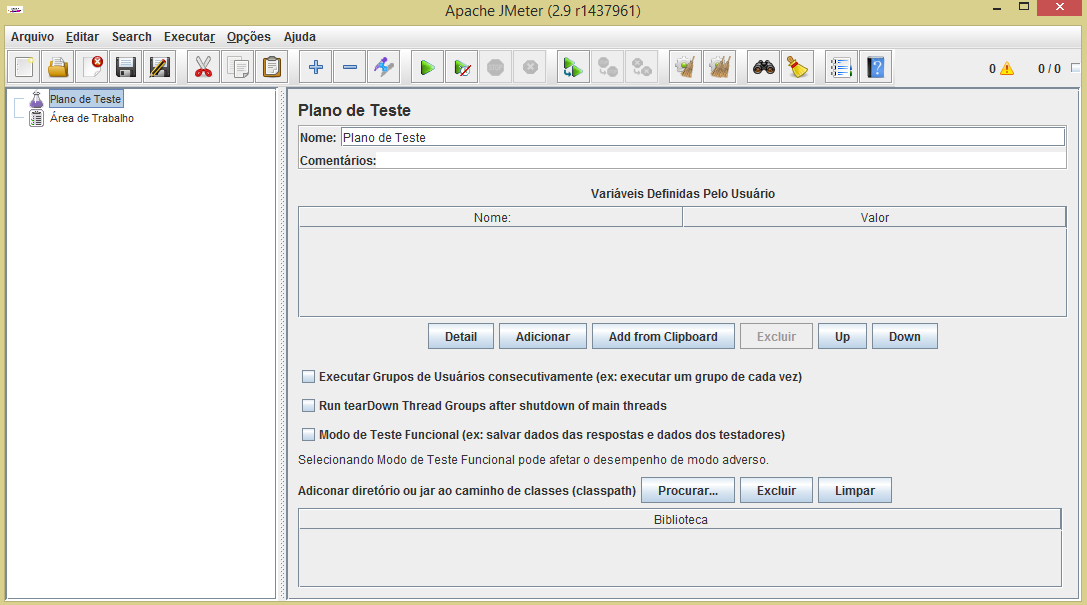
\includegraphics[scale=0.5]{imagens/plantest.png}
    \caption{Exemplo de plano de teste}
    \label{fig:plantest}
    \end{figure}

\subsection{Adicionando usuários virtuais}

Para simular as ações dos usuários o JMeter permite a adição de um componente chamado Grupo de Usuários. Este componente agrega todos os demais elementos necessários para a execução dos testes, controlando as ações de pseudos usuários no
sistema. Para adicioná-lo ao Plano de Teste basta acionar: Editar/Adicionar/\textit{Threads(Users)}/Grupo de Usuários. Conforme ilustra a Figura \ref{fig:grupodeusuarios}.

   \begin{figure}[htb]
    \centering
    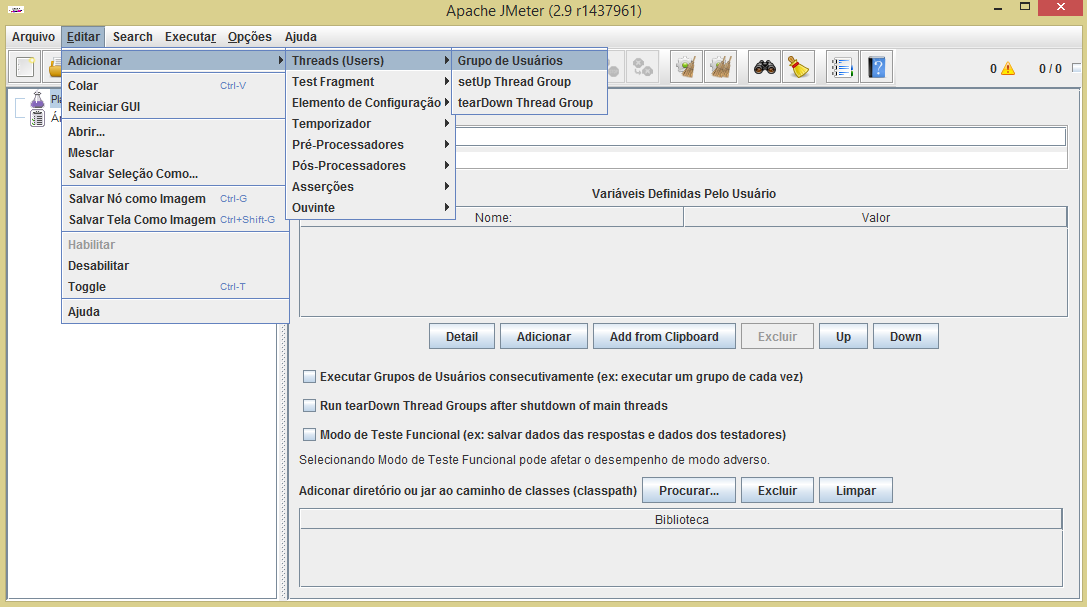
\includegraphics[scale=0.5]{imagens/usergroup.png}
    \caption{Criando grupo de usuários}
    \label{fig:grupodeusuarios}
    \end{figure}


Uma das funcionalidades da tela Grupo de Usuários é controlar o número de usuários que acessaram o sistema. Com isso, foram efetuados testes variando a quantidade de usuários entre 100 e 5000.

\subsection{Configurando acesso ao \textit{cluster} Cassandra}

Para conseguir acessar o \textit{cluster} Cassandra é necessário adicionar o item Cassandra \textit{Properties} aos Elementos de Configuração. Com este elemento é possível definir quais nós do \textit{cluster} serão acessados e em qual porta, qual tipo de interface será utilizada para enviar requisições aos nós do \textit{cluster}, qual o nome do \textit{cluster}, em qual \textit{keyspace} serão realizados os testes, qual o máximo de conexões por nó e qual o tipo de consistência de leitura e escrita serão utilizadas. O caminho para adicionar o item Cassandra \textit{Properties} é: Editar/Adicionar/Elemento de Configuração, conforme Figura \ref{fig:cassandraproperties}.


   \begin{figure}[htb]
    \centering
    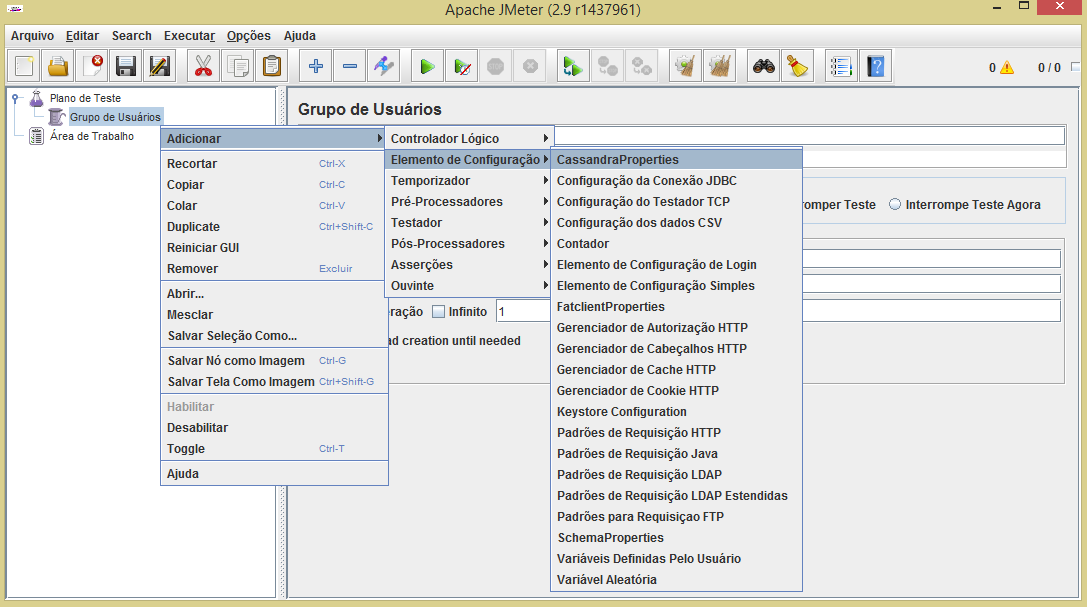
\includegraphics[scale=0.5]{imagens/cassandraprop.png}
    \caption{Propriedades da conexão com Cassandra}
    \label{fig:cassandraproperties}
    \end{figure}


\subsection{Configurando arquivo de dados CSV}

O arquivo \textit{.csv} é utilizado para simular a gravação de dados no Cassandra. As informações contidas neste arquivo são utilizadas para identificar quais variáveis serão gravadas e como elas são delimitadas. A Figura \ref{fig:csvprop}, ilustra a tela de configuração do arquivo \textit{.csv}.

   \begin{figure}[htb]
    \centering
    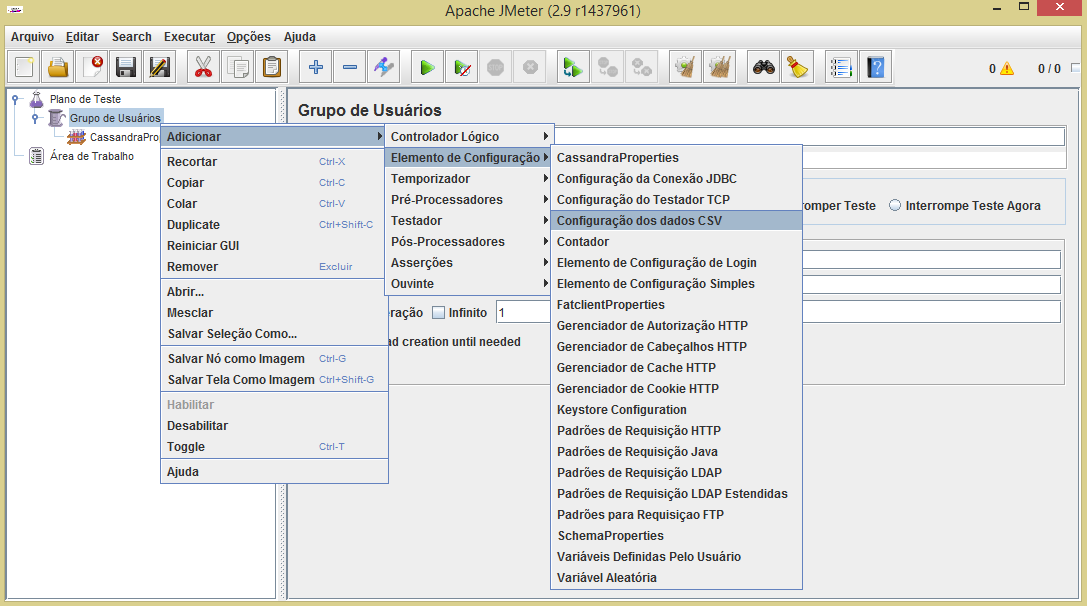
\includegraphics[scale=0.5]{imagens/csvprop.png}
    \caption{Propriedades do arquivo de dados}
    \label{fig:csvprop}
    \end{figure}

\subsection{Configurando a criação das propriedades de schema}

Através do JMeter é possível criar \textit{schemas} no Cassandra para finalidade de testes. Nesta etapa de configuração é possível definir os parâmetros: \textit{column\_family, keys\_cached, rows\_cached}, entre outros, conforme a Figura \ref{fig:schemaprop}.

   \begin{figure}[htb]
    \centering
    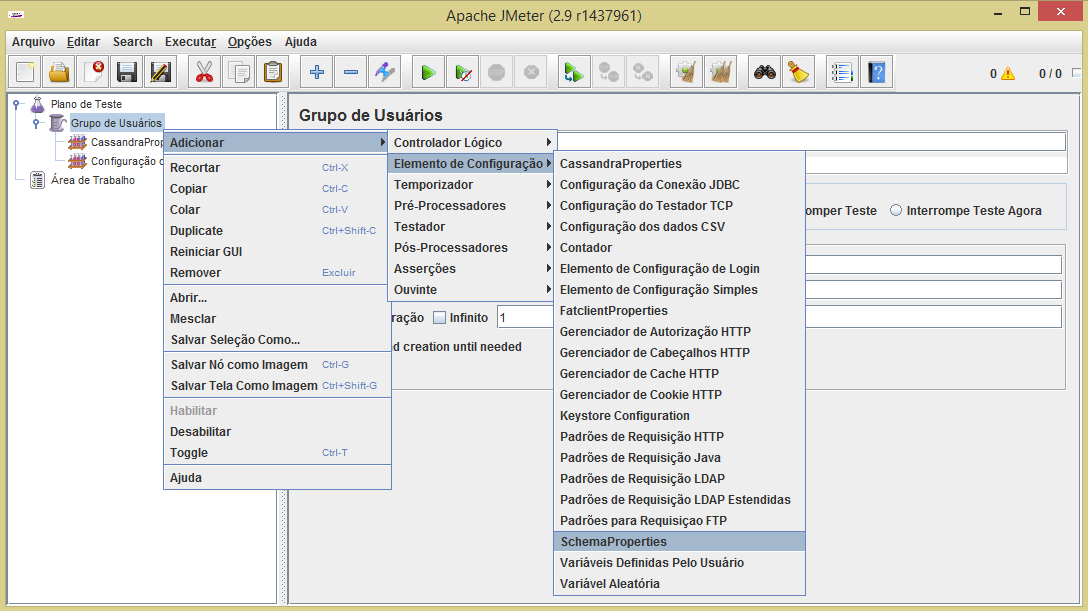
\includegraphics[scale=0.5]{imagens/schemaprop.png}
    \caption{Propriedades do \textit{schema} Cassandra}
    \label{fig:schemaprop}
    \end{figure}

\subsection{Adicionando dados ao \textit{cluster}}

Para adicionar dados ao \textit{cluster} Cassandra o JMeter faz uso de controladores chamados, genericamente, de Testadores. Existem vários tipos de Testadores, para os mais variados tipos de serviços. Para executar a operação de adição de dados ao \textit{cluster} Cassandra utilizou-se o Testador Cassandra \textit{Put}. O caminho para os controladores de requisição é: Editar/Adicionar/Testador, conforme Figura \ref{fig:cassandraput}.


   \begin{figure}[htb]
    \centering
    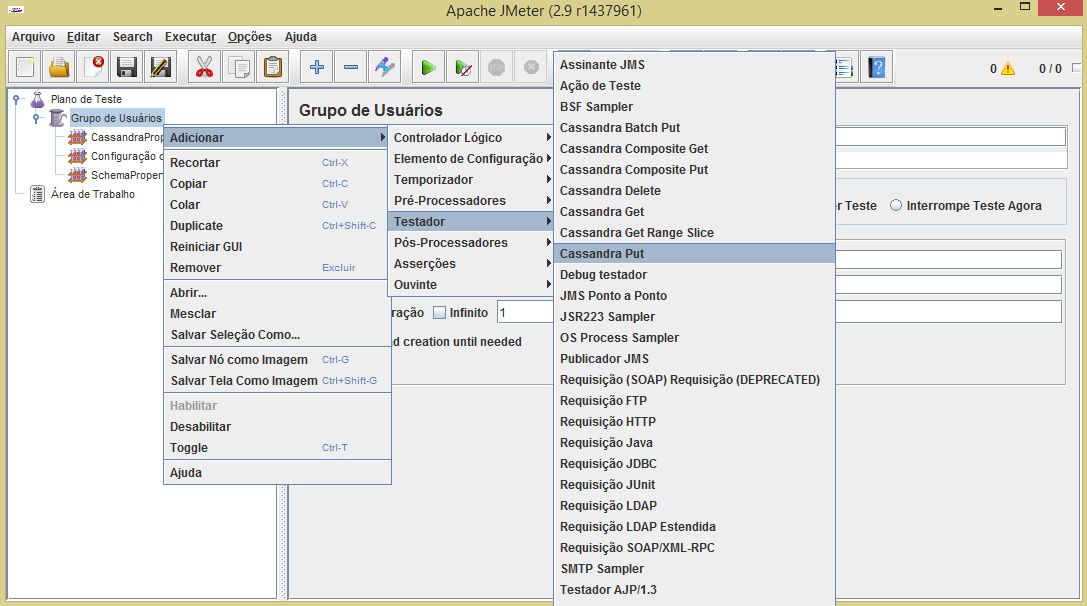
\includegraphics[scale=0.5]{imagens/cassandraput.png}
    \caption{Exemplo de gravação de dados no Cassandra}
    \label{fig:cassandraput}
    \end{figure}

% Analise Performance
\chapter{Revisão sobre análise de desempenho}
\label{cap:analisePerformance}
Neste capítulo são apresentados diversos conceitos relacionados aos métodos escolhidos para se realizar a análise de desempenho ou uma simulação, refletindo o sistema real.

O desempenho  é um critério essencial na elaboração de um projeto, aquisição e utilização de um sistema de computador. Cada avaliação requer um conhecimento íntimo do sistema a ser avaliado e uma seleção cuidadosa de metologia, carga e ferramentas. Além de contar com a experiência do analista que irá realizar a avaliação para que esse possa decidir entre métodos similares e melhores configurações \cite{Jain}.

    Para avaliar um sistema deve-se definir objetivos claros a respeito do que precisa ser avaliado, pois não existe uma forma genérica de avaliação de desempenho. As métricas, carga e metodologia dependem do objetivo a ser atingido e podem variar de um problema para outro.
    
    Então temos que a compreensão do problema é a parte mais importante do projeto de avaliação de desempenho. Envolve grande parte do esforço no desenvolvimento deste. Temos também que considerar quais medidas de desempenho serão utilizadas no projeto. Dependendo do tipo de sistema, podemos ter: MIPS, RISCS e CISCS. Sendo que as duas últimas, tratam da avaliação de processadores.
    
    Na definição do projeto é importante considerar uma carga representativa do problema, pois esta tem impacto significativo nos resultados das avaliações de desempenho. Outro ponto importante de um projeto de avaliação de desempenho é a seleção de técnicas de avaliação que podem ser: medida, simulação e modelagem analítica. A medida é também denominada experimentação direta, a qual consiste na observação direta de sistemas reais. A simulação implica na modelagem de um processo ou sistema, de tal forma que o modelo imite as respostas do sistema real numa sucessão de eventos que ocorrem ao longo do tempo. E a modelagem analítica se baseia no desenvolvimento de um modelo do sistema real, porém com um nível de abstração mais alto que do modelo de simulação.
    
    Existem analistas que costumam superestimar uma determinada técnica sendo que o uso desta pode implicar em coisas como conversões e outras manipulações que tornam os resultados imprecisos.
    
    Considera-se uma boa prática, listar características de carga e do sistema que será avaliado a fim de que a partir desses se extraia os devidos parâmetros de avaliação. Como exemplo de parâmetros de carga temos: número de usuários, padrões de recepção de requisições e prioridades. Dentre os parâmetros, alguns podem variar durante a avaliação; esses parâmetros são chamados de fatores. Como exemplo de fatores, temos o número de usuários. Esses fatores são importantes dado que podem afetar significativamente os resultados da avaliação.
    
    Assim, temos que a seleção apropriada dos números de medidas ou experimentos de simulações a serem conduzidos e os valores dos parâmetros usados em cada experimento podem induzir mais informações nos resultados ou a nenhuma informação relevante dado o mesmo número de experimentos realizados.
    
    É importante considerar um equilíbrio do nível de detalhes das técnicas utilizadas no projeto. Não podem ser muito abrangentes e nem muito específicas. De preferência avaliar o momento certo do uso de uma métrica mais detalhada e do uso de uma de alto nível. Além disso, durante a análise de um sistema, o analista pode se enganar na modelagem e na análise e chegar a resultados incorretos ou então, não apresentar os resultados obtidos de forma adequada. Segundo \citeonline{Jain}, aconselha-se que, inicialmente, se dê preferência a modelos (metodologias) mais simples, que se planeje a melhor forma de apresentar os resultados e que os objetivos de análise e do sistema sejam definidos de forma clara.
    
\section{Seleção de Técnicas e Métricas}
    
    Existem alguns itens que ajudam a decidir qual técnica utilizar (modelagem analítica, medidas ou simulação). Esses itens estão listados na tabela a seguir:
  
  
  
  
  
  
  
  
\begin{table}[h]
\caption{Critérios para seleção e técnicas de avaliação} \cite[p. 31]{Jain}
\label{my-label}
\centering
\resizebox{\textwidth}{!}{%
\begin{tabular}{c|c|c|c|c|}
\cline{2-5}
 & \cellcolor[HTML]{C0C0C0}\textbf{Critério} & \cellcolor[HTML]{C0C0C0}\textbf{Modelagem Analítica} & \cellcolor[HTML]{C0C0C0}\textbf{Simulação} & \cellcolor[HTML]{C0C0C0}\textbf{Medida} \\ \hline
\multicolumn{1}{|c|}{\cellcolor[HTML]{C0C0C0}\textbf{1}} & Estágio & Qualquer & Qualquer & Protótipo Publicado \\ \hline
\multicolumn{1}{|c|}{\cellcolor[HTML]{C0C0C0}\textbf{2}} & Tempo Requerido & Pequeno & Médio & Vários \\ \hline
\multicolumn{1}{|c|}{\cellcolor[HTML]{C0C0C0}\textbf{3}} & Ferramentas & Analistas & Linguagens de Computação & Instrumentação \\ \hline
\multicolumn{1}{|c|}{\cellcolor[HTML]{C0C0C0}\textbf{4}} & Precisão* & Baixo & Moderado & Vários \\ \hline
\multicolumn{1}{|c|}{\cellcolor[HTML]{C0C0C0}\textbf{5}} & Avaliação de \textit{Trade-off} & Fácil & Moderado & Difícil \\ \hline
\multicolumn{1}{|c|}{\cellcolor[HTML]{C0C0C0}\textbf{6}} & Custo & Pequeno & Médio & Alto \\ \hline
\multicolumn{1}{|c|}{\cellcolor[HTML]{C0C0C0}\textbf{7}} & Viabilidade Comercial & Baixo & Médio & Alto \\ \hline
\end{tabular}
}
\end{table}
  
    
    A principal chave a ser considerada na decisão da técnica de avaliação é o estágio do ciclo de vida em que se encontra o sistema. Desta forma, pode-se ordenar as técnicas por modelagem analítica, medidas e  simulações. A modelagem analítica requer muitas simplificações ou suposições, enquanto as medidas estão sujeitas a imprevistos e a configuração do sistema sobre o problema pode ser irreprodutível. Já as simulações, apesar de terem um melhor detalhamento dos resultados, apresentam um alto custo de execução.
    
    Logo, tem-se que considerar também o tamanho do escopo dos experimentos, dados os objetivos a serem alcançados lembrando que experimentos com escopos pequenos podem induzir a resultados incoerentes à aplicação real.
    
    Assim, deve-se ressaltar o seguinte mandamento nas avaliações de desempenho: \textit{até que sejam validados, todos os resultados da avaliação são suspeitos} \cite{Jain} e para avaliação de cada técnica é aconselhável o uso de uma segunda técnica.
    
    
\section{Seleção de Métricas de Desempenho}
    
    Para cada experimento de desempenho, um grupo de critérios de desempenho ou métrica devem ser escolhidos.
    Uma forma para preparar este grupo é listar os serviços oferecidos pelo sistema. Para cada requisição do sistema, existem diversas saídas possíveis e geralmente essas saídas podem ser classificadas em 3 categorias como mostrada na tabela da seção anterior.
    O sistema pode executar o serviço de forma correta, incorreta ou ainda se recusar a executá-lo. Por exemplo, dado um servidor web ele pode não responder a uma requisição, se estiver fora de operação, ou responder de forma incorreta, redirecionando à um destino incorreto, ou ainda, executar exatamente como esperado.
    
    \begin{figure}[htb]
    \centering
    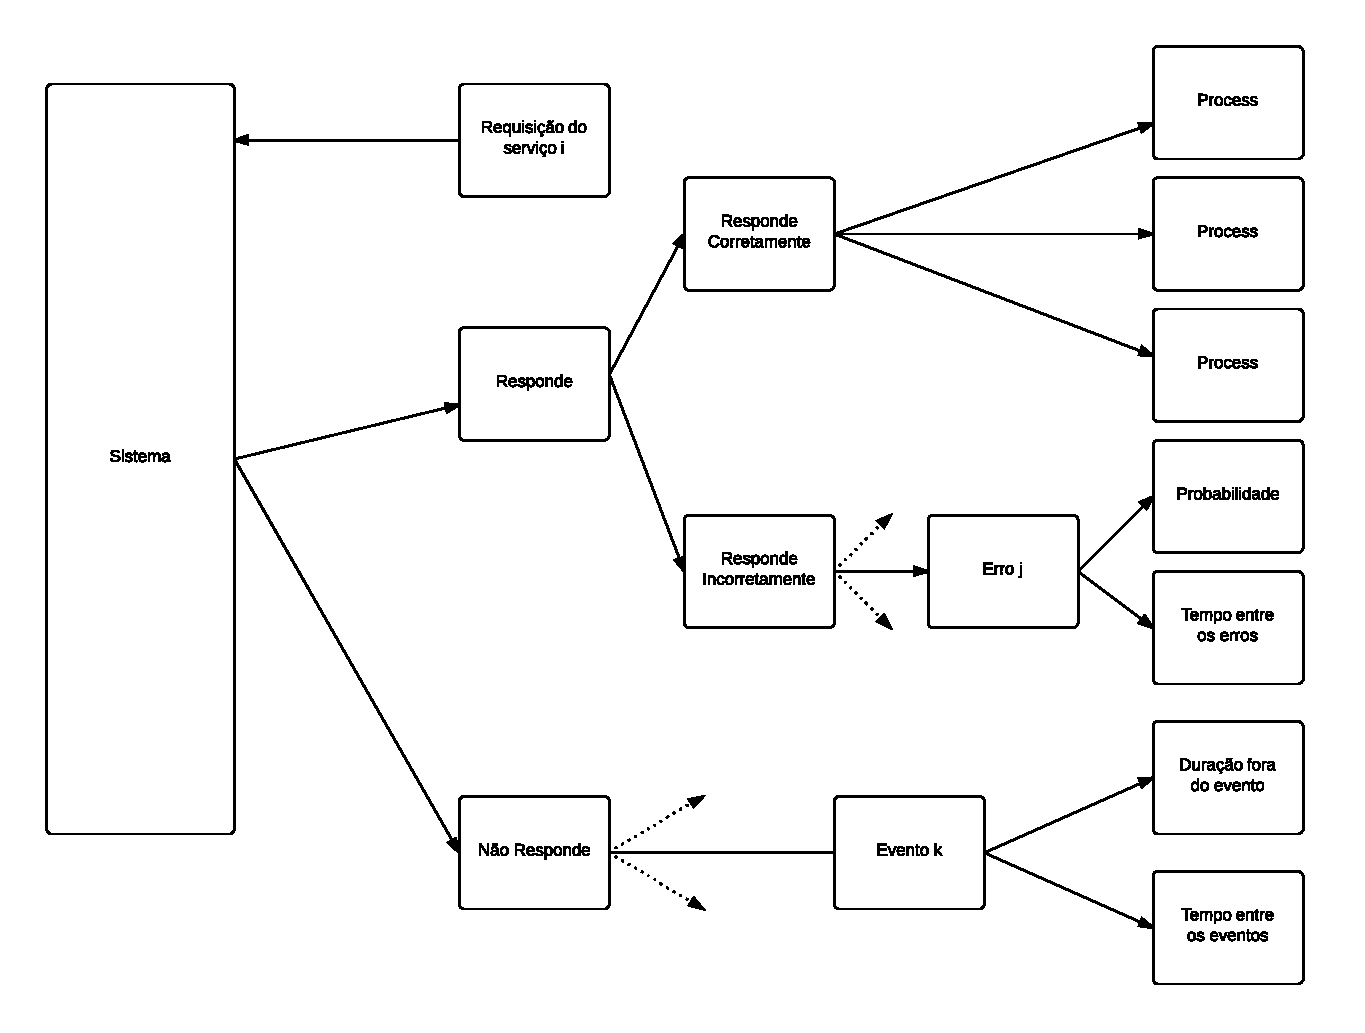
\includegraphics[scale=0.65]{imagens/saidarequisicao.pdf}
    \caption{Três possíveis resultados para requisições de serviços} \cite[p. 33]{Jain}
    \end{figure}

\section{Métricas de Desempenho Comumente Utilizadas}
\label{sec:metricas}
    
   Existem 3 métricas de desempenho mais comumente utilizadas, porém estas definições podem variar de acordo com o projeto \cite{Jain}. São elas:
    \begin{itemize}
    \item Tempo de Resposta: é definido como o intervalo entre a requisição do usuário e a resposta do sistema;
    \item Capacidade: relaciona a capacidade de processamento (requisições por unidade de tempo)  com o tempo de resposta do sistema e
    \item Eficiência: é a eficiência dos multi-processadores dos sistema. A razão entre o desempenho de um sistema \textit{n-processador} de um sistema \textit{one-processador} é a sua eficiência. O desempenho é geralmente medido em termos de MIPS ou MFLOPS.
    \end{itemize}

% ---
% primeiro capitulo de Resultados
% ---
\chapter{Simulações e Resultados}
\label{cap:resultados}
O ambiente descrito no Capítulo \ref{cap:ambExperimental} foi utilizado para a realização das simulações e a ferramenta JMeter foi executada dentro do servidor Maritaca para evitar que o tempo de latência de Internet impactasse nos experimentos.

Em todas as simulações, o balanceamento de carga dos testes foi realizado automaticamente pelo JMeter e a criação dos dados a serem gravados foi feita utilizando uma função randômica do próprio simulador. A consistência de escrita dos dados era \textit{ONE}\footnote{Caracteriza a gravação dos dados em apenas um nó, sem replicação.} quando havia apenas um nó e \textit{TWO}\footnote{Caracteriza a gravação dos dados em um nó e replicação do mesmo em outro nó.} quando o \textit{cluster} possuia mais que um nó. 

Cada nó do \textit{cluster} de dados poderia receber até 100 conexões simultâneas e o tipo de cliente utilizado na conexão do simulador com a base de dados foi o \textit{ThriftConnection}, devido ao Cassandra utilizar este cliente como padrão.

O tempo de duração das requisições de cada teste foi de 60 segundos, sendo que entre cada um dos testes havia um intervalo de 30 segundos, no qual era feito o \textit{flush} dos dados gravados temporariamente pelo JMeter. Em todos os cenários testou-se o comportamento da base de dados Cassandra quando o acesso simultâneo de usuários variava de 1 a 4000 usuários.

\section{Cenário 1}

Neste cenário, as operações de inserção de dados no Cassandra foram realizadas com o Cassandra operando apenas com um nó.
Para isto, utilizou-se um \textit{host} contendo apenas o Cassandra instalado.

    \begin{figure}[H]
    \centering
    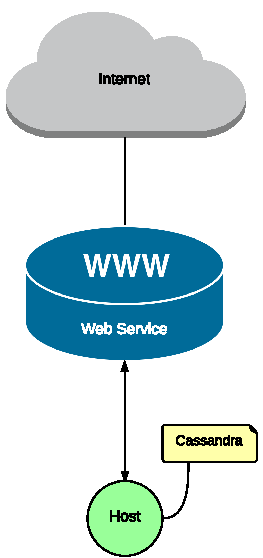
\includegraphics[scale=0.60]{imagens/BD-1Host.pdf}
    \caption{Cenário 1}
    \label{fig:bd1host}
    \end{figure} 

\section{Cenário 2}
Neste cenário, as operações de inserção de dados no Cassandra foram realizadas com o Cassandra operando apenas com um nó.
Para isto, utilizou-se um \textit{guest} contendo apenas o Cassandra instalado. O objetivo neste cenário era avaliar possíveis diferenças entre \textit{host} e \textit{guest}.

    \begin{figure}[H]
    \centering
    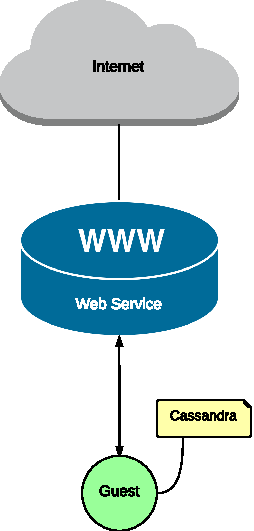
\includegraphics[scale=0.60]{imagens/BD-1Guest.pdf}
    \caption{Cenário 2}
    \label{fig:bd1guest}
    \end{figure} 

Com os cenários 1 e 2 buscou-se ver o comportamento e a carga suportada por esse ambiente para que pudéssemos compará-lo com o terceiro cenário.

\section{Cenário 3}
Neste cenário, as operações de inserção de dados no Cassandra foi realizada com o Cassandra operando com um \textit{cluster} contendo 2 nós.
Para isto, utilizou-se 2 \textit{host} contendo apenas o Cassandra instalado.
Essas mudanças visavam verificar a possível melhora no serviço oferecido com a inclusão de novas máquinas aos \textit{clusters}, utilizando-se assim da elasticidade presente nos ambientes de computação em nuvem.

    \begin{figure}[H]
    \centering
    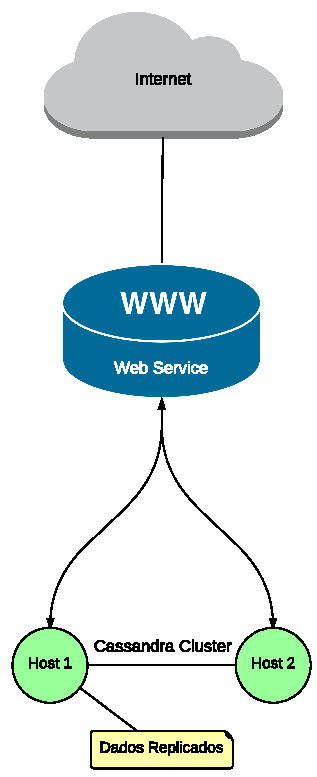
\includegraphics[scale=0.60]{imagens/BD-2Host.pdf}
    \caption{Cenário 3}
    \label{fig:bd2host}
    \end{figure} 
    
    
\section{Cenário 4}
Neste cenário, as operações de inserção de dados no Cassandra foi realizada com o Cassandra operando com um \textit{cluster} contendo 2 nós.
Para isto, utilizou-se 2 \textit{guest} contendo apenas o Cassandra instalado.
Com este cenário foi possível comparar a elasticidade entre ambientes configurados apenas com \textit{hosts} e em ambientes configurados apenas com \textit{guests}.

    \begin{figure}[H]
    \centering
    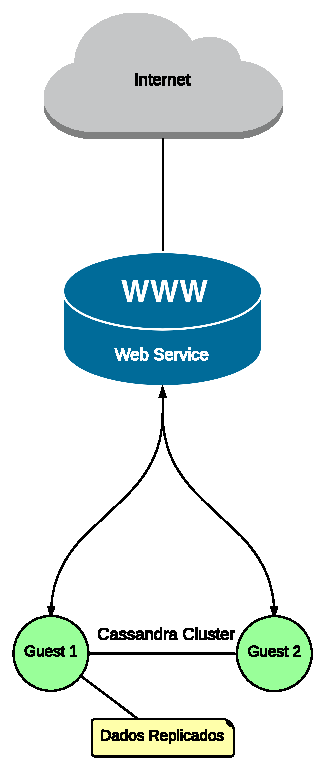
\includegraphics[scale=0.60]{imagens/BD-2Guest.pdf}
    \caption{Cenário 4}
    \label{fig:bd2guest}
    \end{figure} 


\section{Cenário 5}
Neste cenário, as operações de inserção de dados no Cassandra foram realizadas com o Cassandra operando com um \textit{cluster} contendo 2 nós.
Para isto, utilizou-se um \textit{host} e um \textit{guest} contendo apenas o Cassandra instalado, conforme a Figura \ref{fig:bd1host1guest}.

Essas mudanças visavam verificar a comunicação entre \textit{clusters} configurados mesclando \textit{hosts} e \textit{guests} e avaliar o serviço oferecido com a inclusão de novas máquinas aos clusters, utilizando-se assim da elasticidade presente nos ambientes de computação em nuvem.

    \begin{figure}[H]
    \centering
    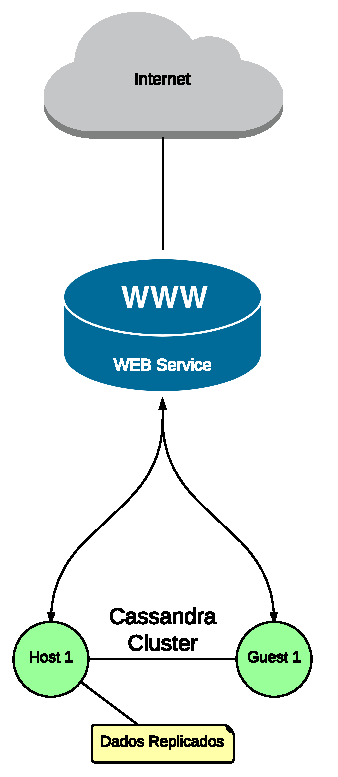
\includegraphics[scale=0.60]{imagens/BD-1Host1Guest.pdf}
    \caption{Cenário 5}
    \label{fig:bd1host1guest}
    \end{figure} 



\section{Cenário 6}
Para o último cenário, definiu-se uma configuração mais comum de observar em aplicações de grande porte, onde a elasticidade das \textit{guests} é utilizada em larga escala. Logo, as operações de inserção de dados no Cassandra foi realizada com o Cassandra operando com um \textit{cluster} contendo 4 nós.
Para isto, utilizou-se 4 \textit{guests} contendo apenas o Cassandra instalado.

    \begin{figure}[H]
    \centering
    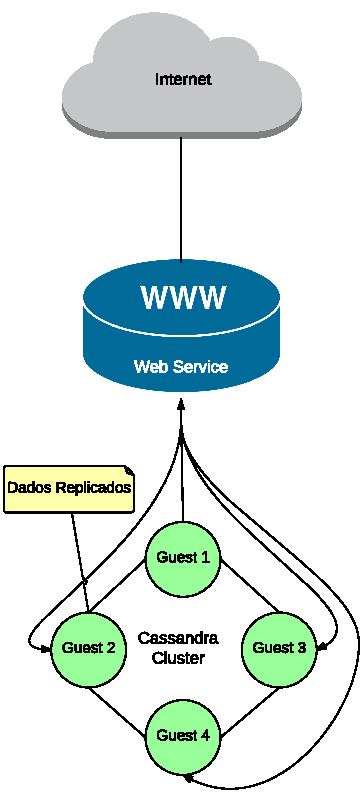
\includegraphics[scale=0.60]{imagens/BD-4Guest.pdf}
    \caption{Cenário 6}
    \label{fig:bd4guest}
    \end{figure}


\section{Resultados}

A Tabela \ref{tab:am} se refere a quantidade de pacotes gravados na base de dados, em 60 segundos.

\begin{table}[ht]
\centering
\caption{Quantidade de amostras gravadas}
\label{tab:am}
\begin{tabular}{|
>{\columncolor[HTML]{C0C0C0}}c |c|c|c|c|c|c|}
\hline
Usuários & \cellcolor[HTML]{C0C0C0}Cenário 1 & \cellcolor[HTML]{C0C0C0}Cenário 2 & \cellcolor[HTML]{C0C0C0}Cenário 3 & \cellcolor[HTML]{C0C0C0}Cenário 4 & \cellcolor[HTML]{C0C0C0}Cenário 5 & \cellcolor[HTML]{C0C0C0}Cenário 6 \\ \hline
1 & 6229 & 6178 & 6097 & 14689 & 7838 & 7126 \\ \hline
10 & 24053 & 34834 & 47324 & 43296 & 44783 & 45340 \\ \hline
50 & 30146 & 41400 & 46469 & 47060 & 44277 & 36392 \\ \hline
100 & 41831 & 42203 & 43928 & 43755 & 43316 & 35651 \\ \hline
250 & 39667 & 43661 & 40750 & 44406 & 40436 & 37234 \\ \hline
500 & 42179 & 39367 & 41925 & 43392 & 39206 & 37514 \\ \hline
750 & 40617 & 40840 & 37081 & 41931 & 41035 & 36169 \\ \hline
1000 & 40904 & 40669 & 37550 & 41995 & 40007 & 38508 \\ \hline
1250 & 40341 & 41916 & 40454 & 43294 & 39681 & 36632 \\ \hline
1500 & 39448 & 42382 & 38359 & 41300 & 38146 & 39555 \\ \hline
1750 & 41258 & 39857 & 37295 & 41564 & 40696 & 40452 \\ \hline
2000 & 42677 & 41467 & 37612 & 41544 & 38236 & 37361 \\ \hline
2250 & 43511 & 42758 & 39323 & 38937 & 39334 & 36440 \\ \hline
2500 & 39481 & 35500 & 32545 & 32982 & 30695 & 35017 \\ \hline
2750 & 36579 & 35517 & 31575 & 33886 & 29995 & 33270 \\ \hline
3000 & 34654 & 34590 & 32114 & 35230 & 32919 & 31941 \\ \hline
3250 & 36240 & 34824 & 31875 & 34220 & 31856 & 31560 \\ \hline
3500 & 33632 & 35368 & 33049 & 34827 & 31900 & 29891 \\ \hline
3750 & 28991 & 36347 & 34037 & 36161 & 33386 & 24095 \\ \hline
4000 & 26672 & 34773 & 34672 & 33493 & 33339 & 20970 \\ \hline
\end{tabular}
\end{table}

Após tabulados os dados, plotou-se o gráfico exibido na Figura \ref{fig:am} para possibilitar uma melhor avaliação dos resultados.




    \begin{figure}[!h]
    \centering
    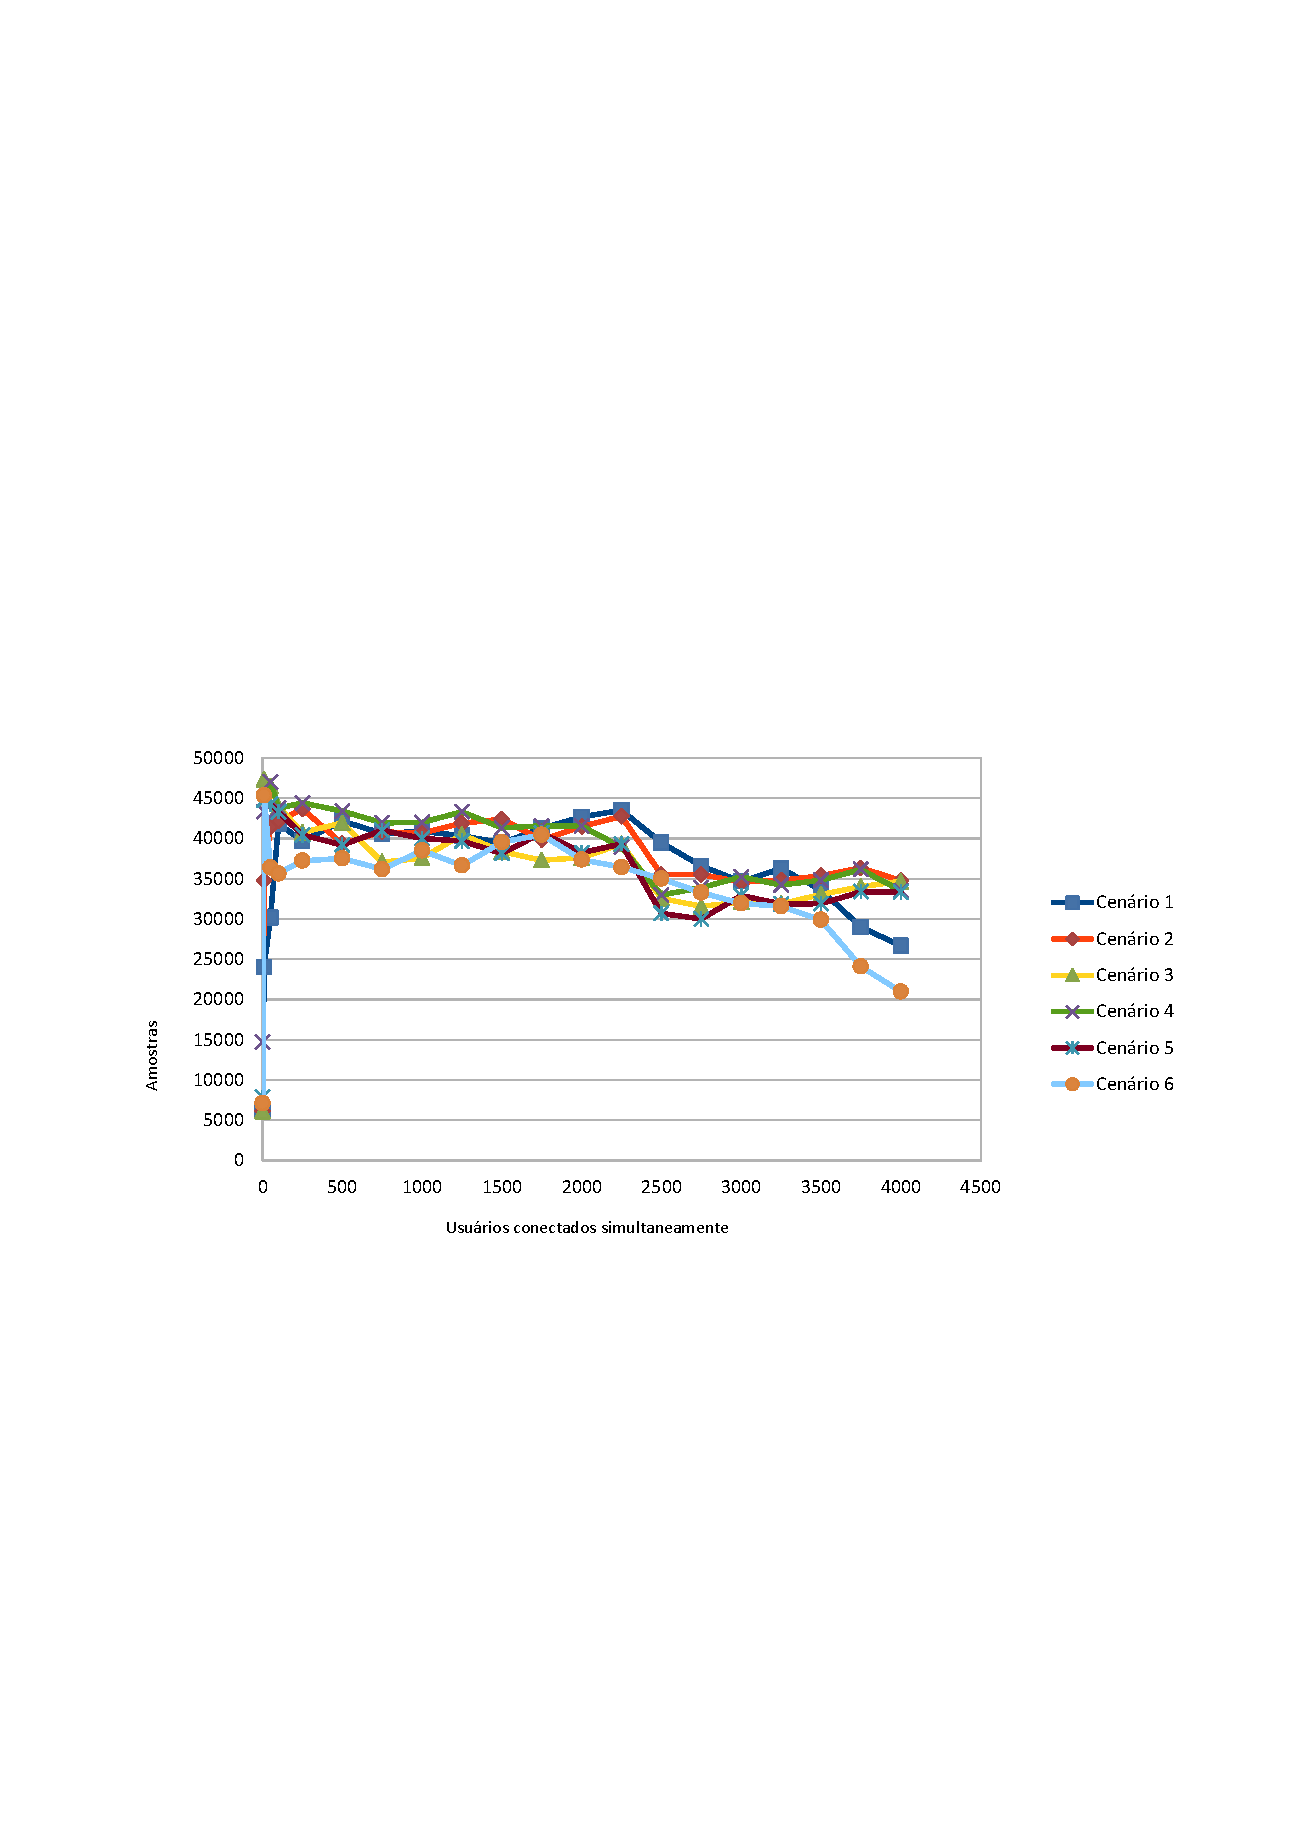
\includegraphics[scale=0.85]{imagens/amXmin.pdf}
    \caption{Quantidade de amostras gravadas por minuto}
    \label{fig:am}
    \end{figure}

Também analisou-se a quantidade de erros gerado com aumento do número de usuários, conectados simultaneamente à base de dados Cassandra, conforme a Tabela \ref{tab:erro}.


\begin{table}[ht]
\centering
\caption{Porcentagem de erro na gravação de pacotes}
\label{tab:erro}
\begin{tabular}{|
>{\columncolor[HTML]{C0C0C0}}c |c|c|c|c|c|c|}
\hline
Usuários & \cellcolor[HTML]{C0C0C0}Cenário 1 & \cellcolor[HTML]{C0C0C0}Cenário 2 & \cellcolor[HTML]{C0C0C0}Cenário 3 & \cellcolor[HTML]{C0C0C0}Cenário 4 & \cellcolor[HTML]{C0C0C0}Cenário 5 & \cellcolor[HTML]{C0C0C0}Cenário 6 \\ \hline
1 & 0 & 0 & 0 & 0 & 0 & 0 \\ \hline
10 & 0 & 0 & 0 & 0 & 0 & 0 \\ \hline
50 & 0 & 0 & 0 & 0 & 0 & 0 \\ \hline
100 & 0 & 0 & 0 & 0 & 0 & 0 \\ \hline
250 & 0 & 0 & 0 & 0 & 0 & 0 \\ \hline
500 & 0 & 0 & 0 & 0 & 0 & 0 \\ \hline
750 & 0 & 0 & 0 & 0 & 0 & 0 \\ \hline
1000 & 0 & 0 & 0 & 0 & 0 & 0 \\ \hline
1250 & 0 & 0 & 0 & 0 & 0 & 0 \\ \hline
1500 & 0 & 0 & 0 & 0 & 0 & 0 \\ \hline
1750 & 0 & 0 & 0 & 0 & 0 & 0 \\ \hline
2000 & 0 & 0 & 0 & 0 & 0 & 0 \\ \hline
2250 & 10 & 0 & 0 & 8 & 0 & 3 \\ \hline
2500 & 16 & 13 & 19 & 20 & 24 & 9 \\ \hline
2750 & 17 & 16 & 21 & 21 & 27 & 14 \\ \hline
3000 & 15 & 15 & 19 & 18 & 23 & 15 \\ \hline
3250 & 13 & 13 & 17 & 16 & 20 & 15 \\ \hline
3500 & 22 & 12 & 15 & 14 & 18 & 22 \\ \hline
3750 & 30 & 11 & 14 & 13 & 16 & 36 \\ \hline
4000 & 37 & 12 & 13 & 20 & 16 & 46 \\ \hline
\end{tabular}
\end{table}


Os erros de gravação foram plotados variando o cenário utilizado e a quantidade de usuários, conforme a Figura \ref{fig:erro}. 


    \begin{figure}[H]
    \centering
    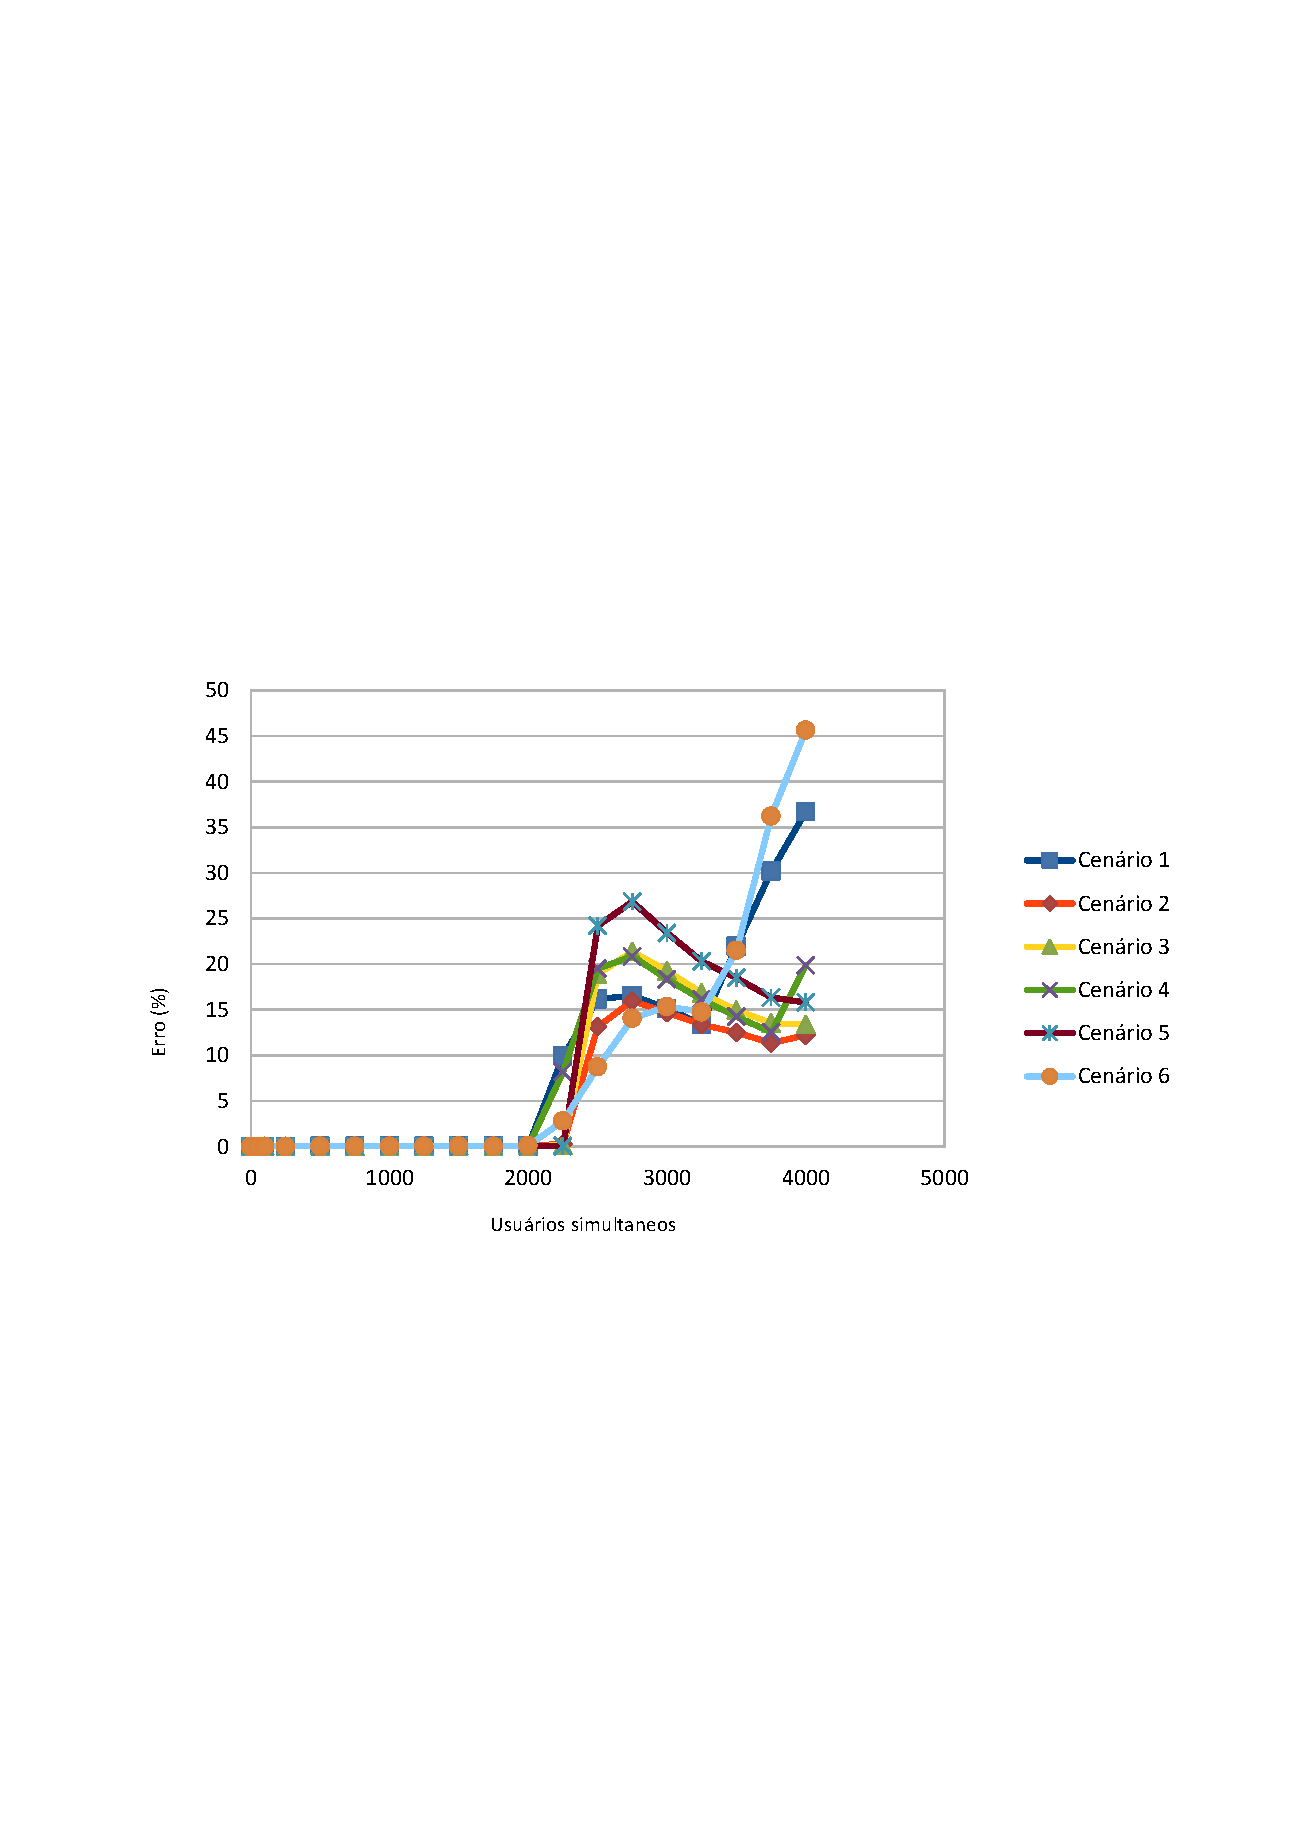
\includegraphics[scale=0.85]{imagens/erroXmin.pdf}
    \caption{Porcentagem de erro na gravação de pacotes}
    \label{fig:erro}
    \end{figure}
    
    
Com os dados obtidos nestas duas avaliações iniciais (Figura \ref{fig:am} e \ref{fig:erro}), não foi possível observar a escalabilidade da base de dados, porém, notou-se que a partir de 2000 usuários, todos os cenários tiveram um aumento considerável do número de erros e consequentemente uma diminuição do número de requisições atendidas com sucesso. 

Este comportamento também foi notado em todos os gráficos de média e desvio padrão, nos quais houve um aumento expressivo do desvio padrão a partir desta quantidade de usuários, conforme as Figuras \ref{fig:dvp1}, \ref{fig:dvp2}, \ref{fig:dvp3}, \ref{fig:dvp4}, \ref{fig:dvp5} e \ref{fig:dvp6}. 

    \begin{figure}[H]
    \centering
    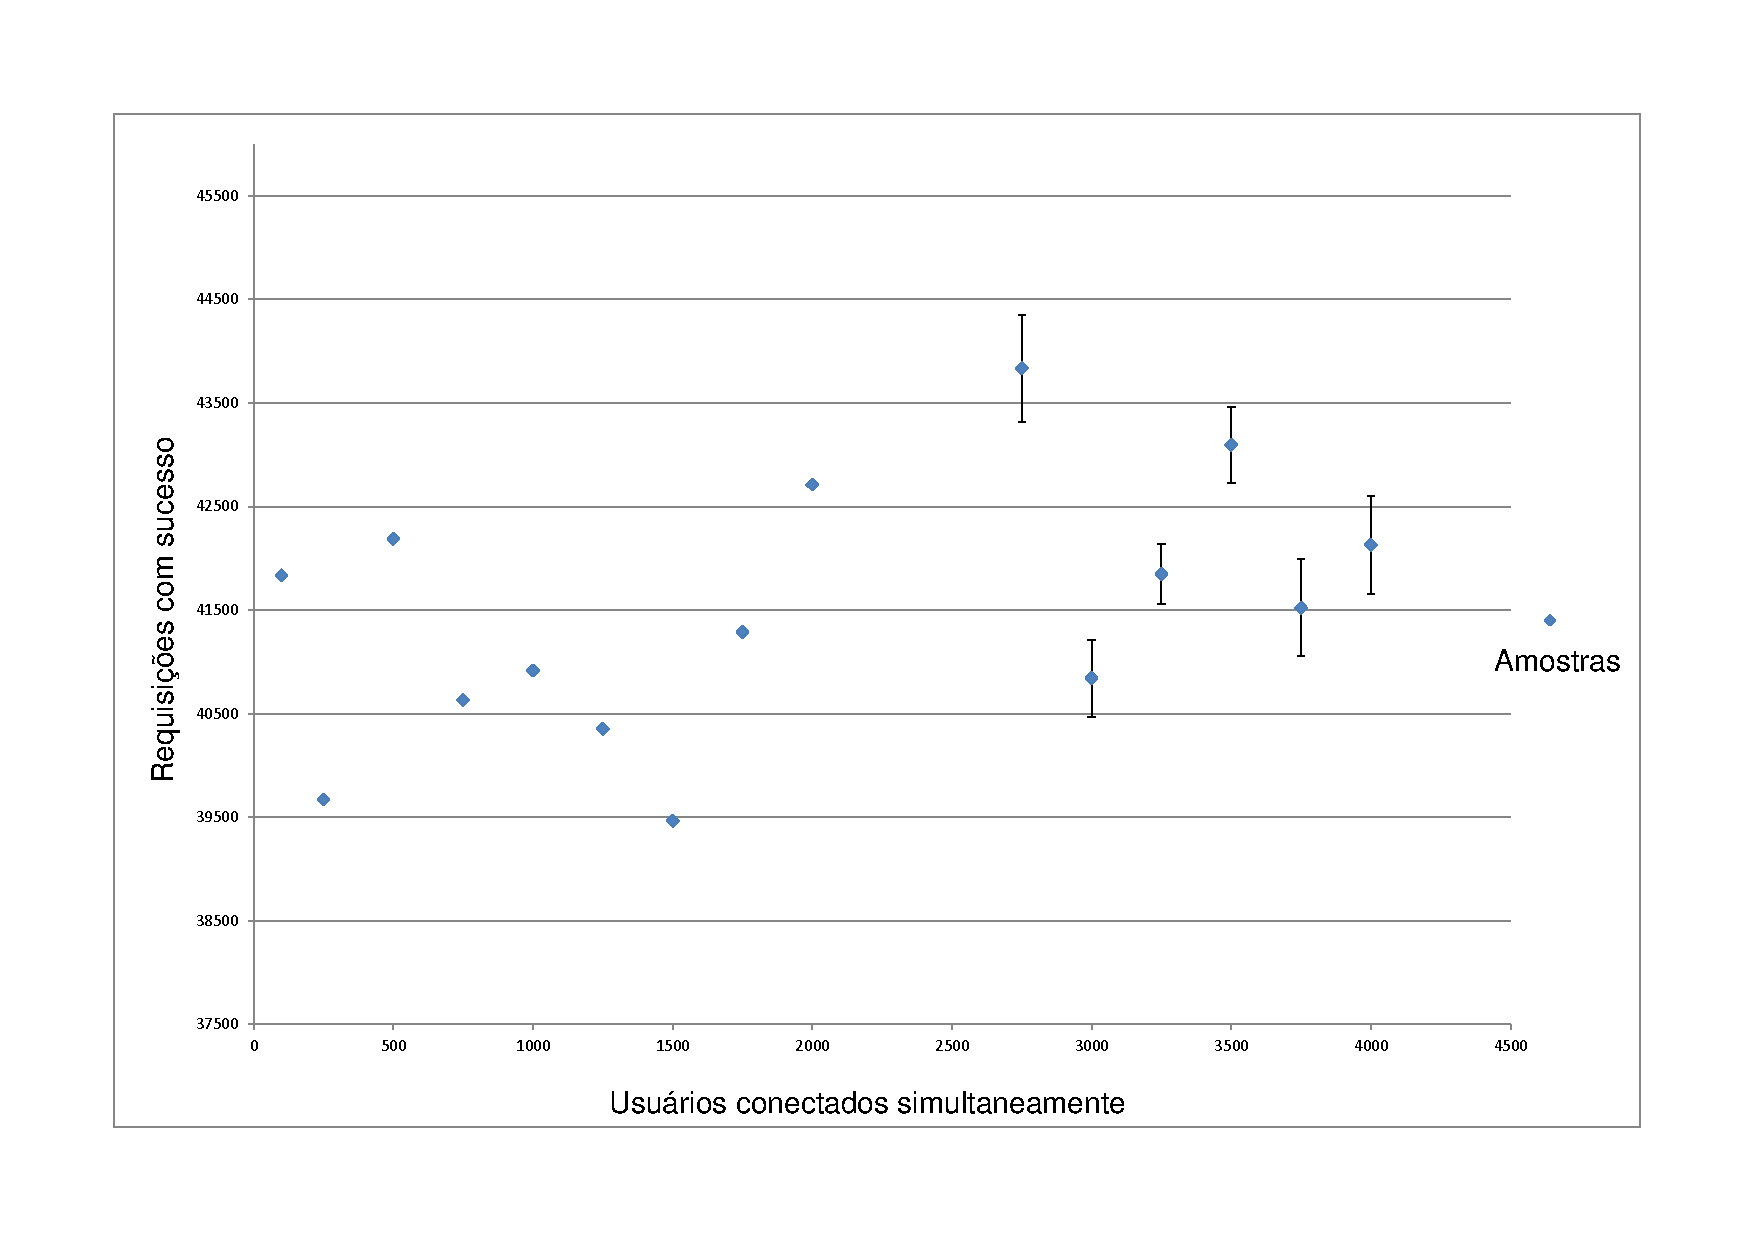
\includegraphics[scale=0.50]{imagens/dvp1.pdf}
    \caption{Média e desvio padrão do Cenário 1}
    \label{fig:dvp1}
    \end{figure}
    
        \begin{figure}[H]
    \centering
    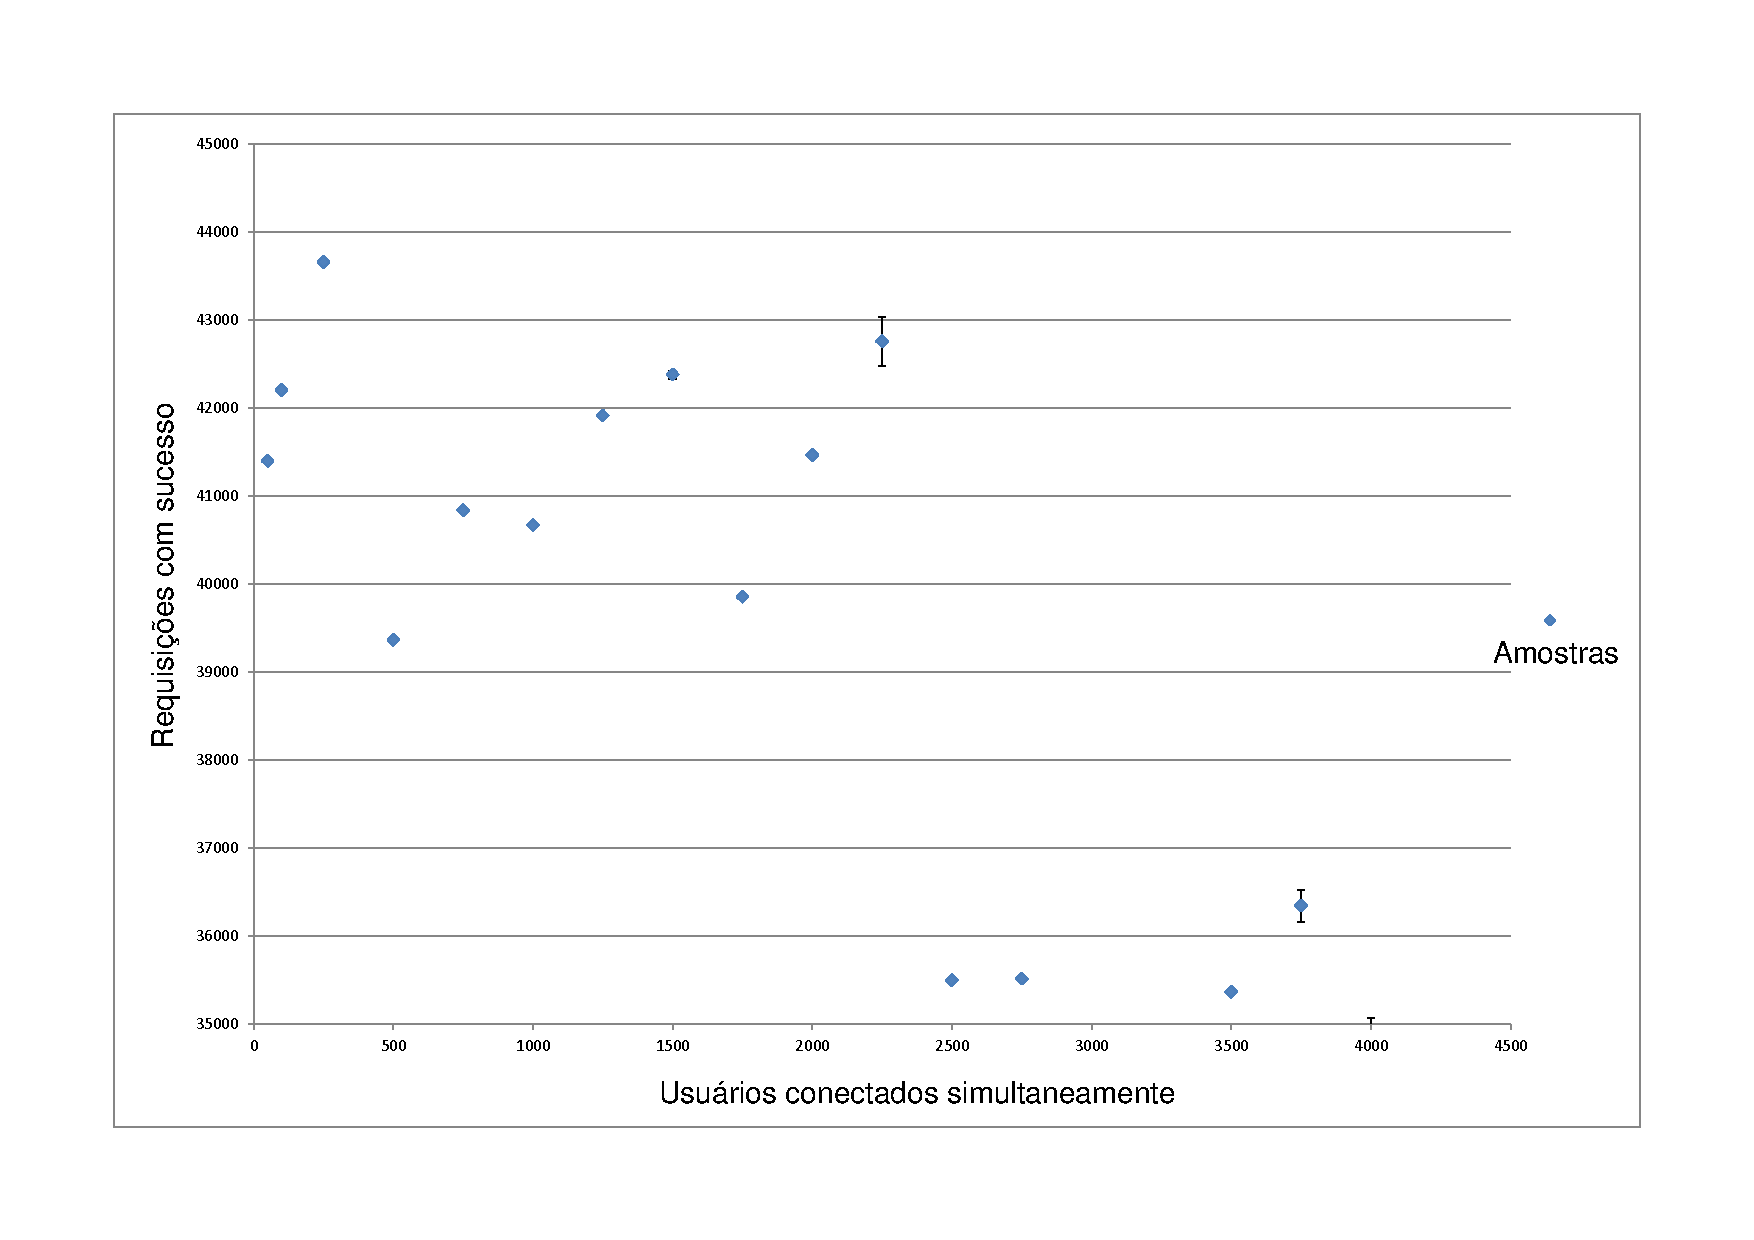
\includegraphics[scale=0.5]{imagens/dvp2.pdf}
    \caption{Média e desvio padrão do Cenário 2}
    \label{fig:dvp2}
    \end{figure}
    
        \begin{figure}[H]
    \centering
    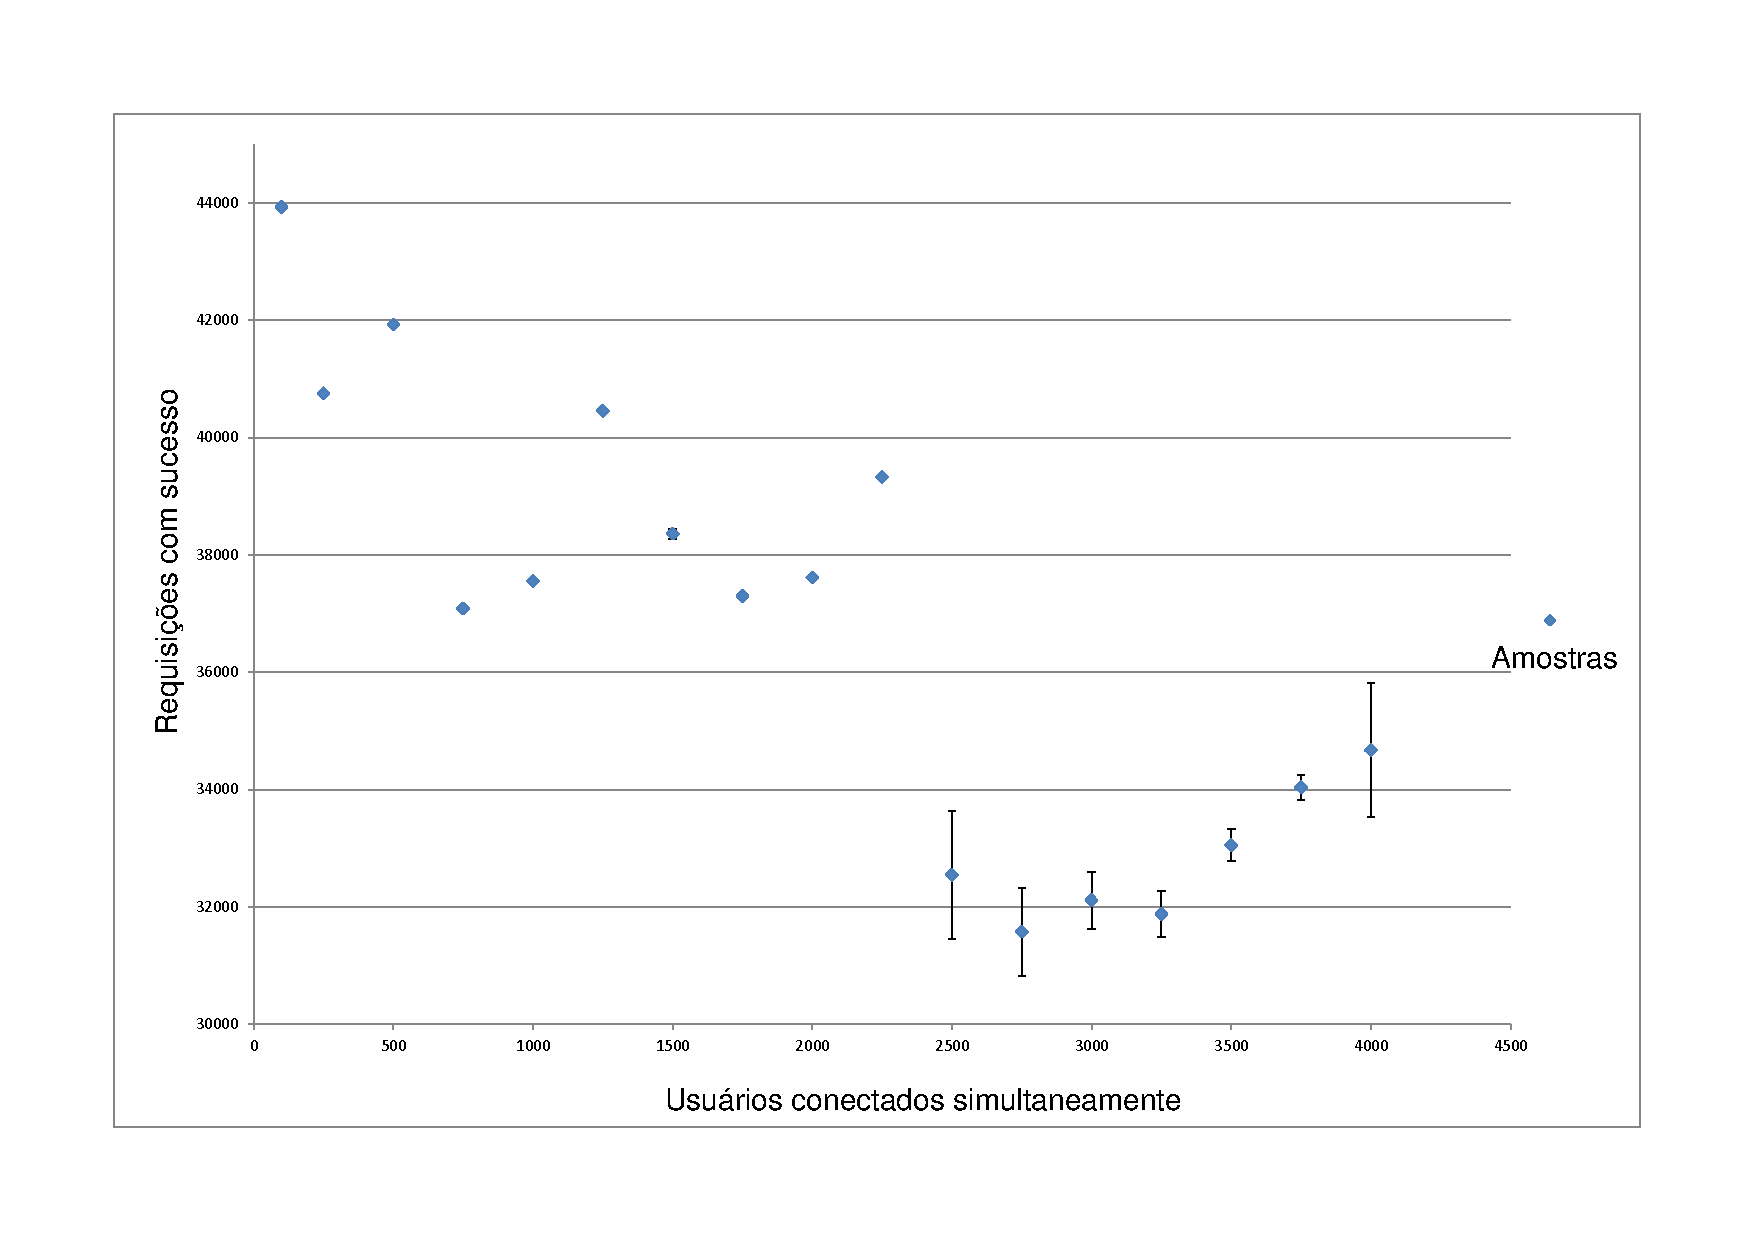
\includegraphics[scale=0.5]{imagens/dvp3.pdf}
    \caption{Média e desvio padrão do Cenário 3}
    \label{fig:dvp3}
    \end{figure}
    
        \begin{figure}[H]
    \centering
    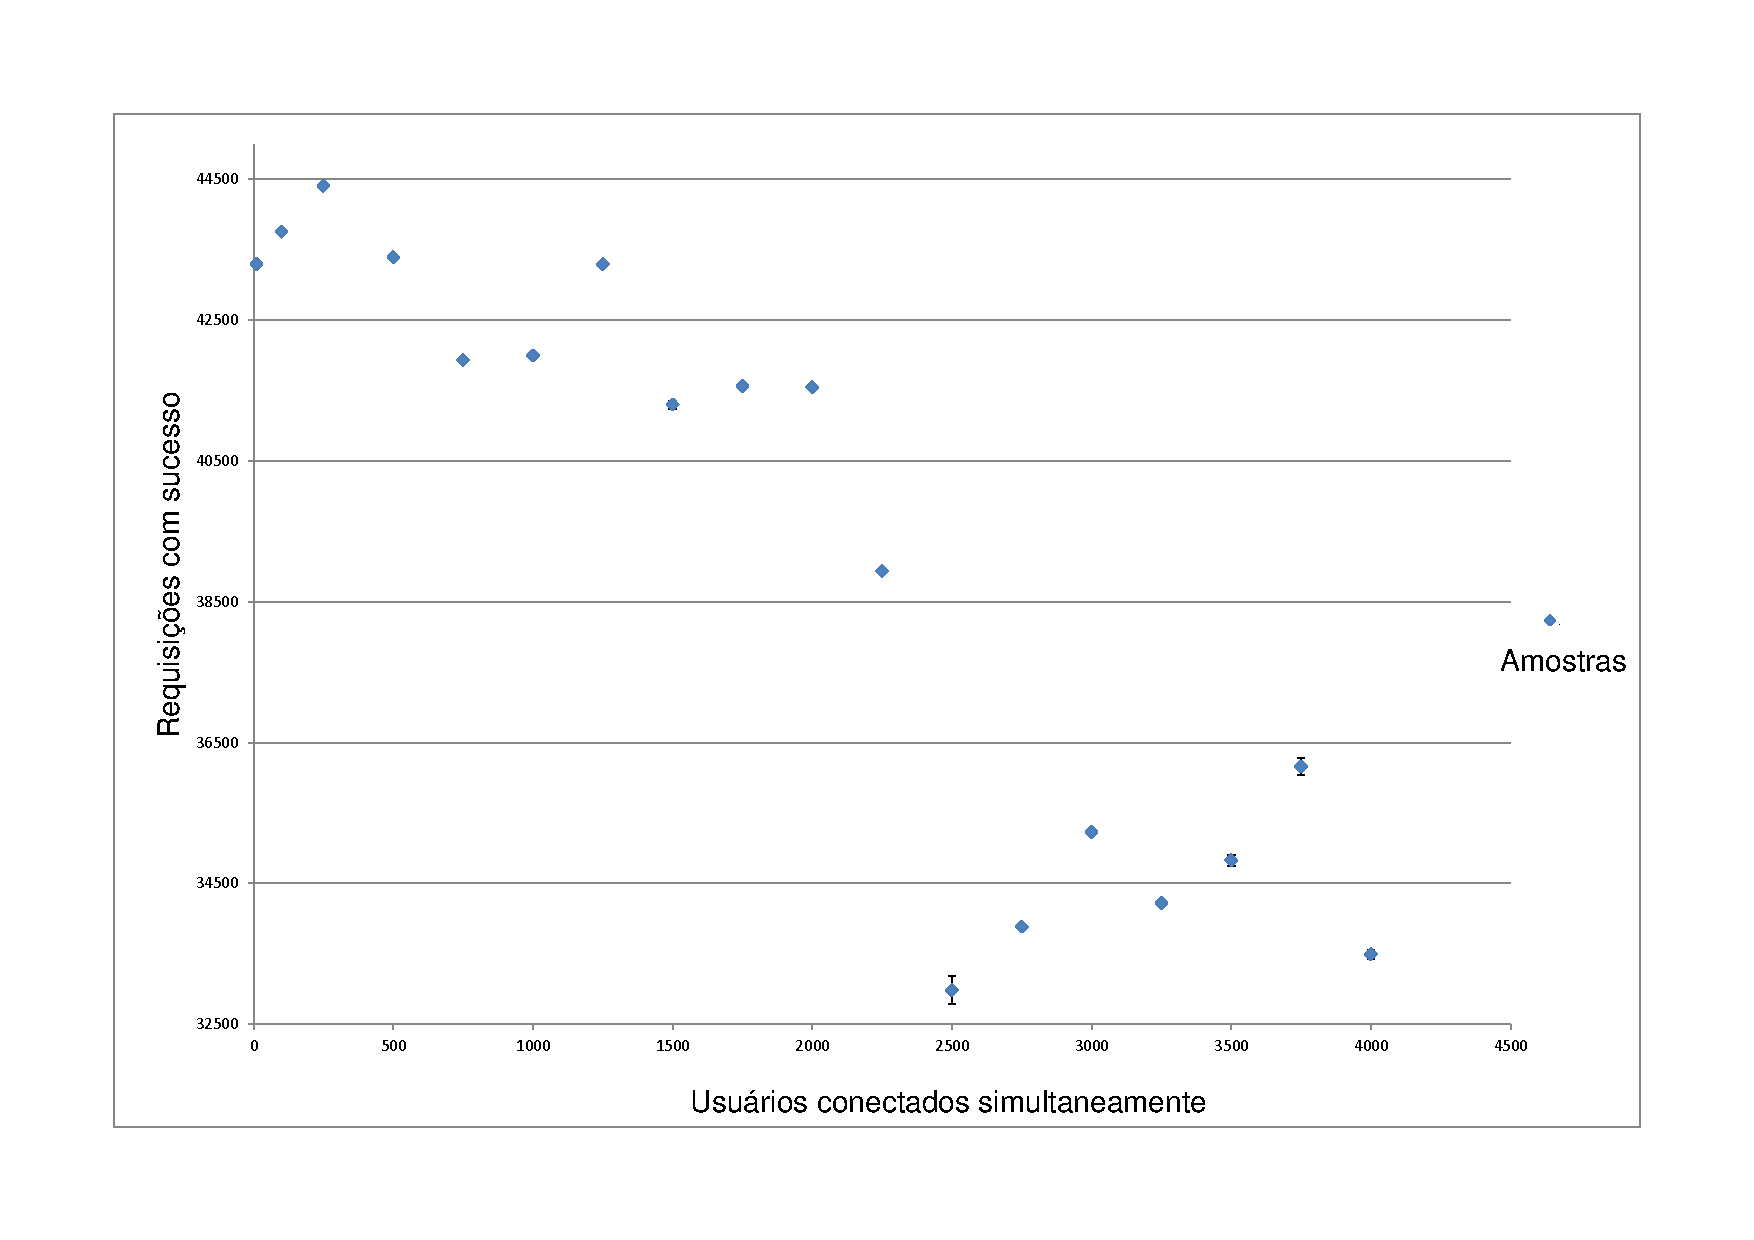
\includegraphics[scale=0.5]{imagens/dvp4.pdf}
    \caption{Média e desvio padrão do Cenário 4}
    \label{fig:dvp4}
    \end{figure}
    
        \begin{figure}[H]
    \centering
    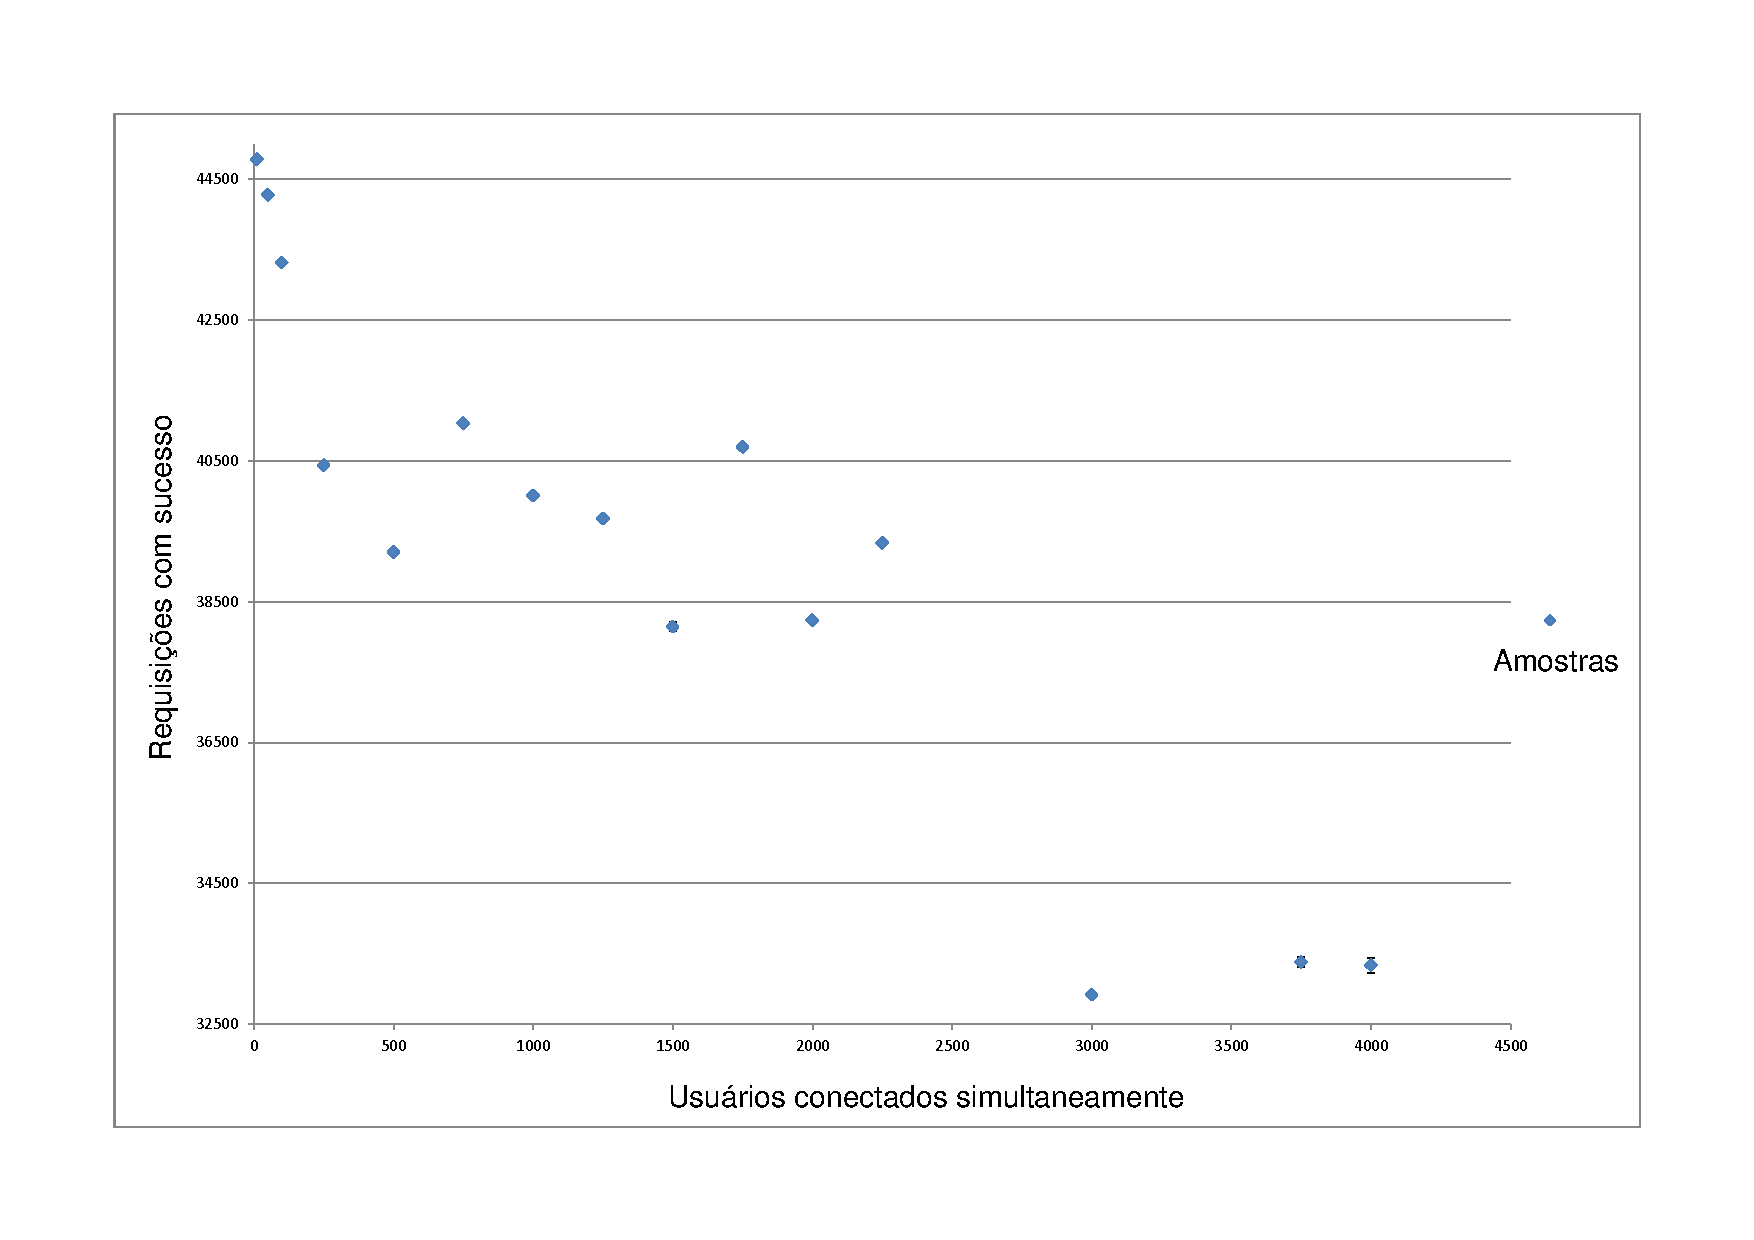
\includegraphics[scale=0.5]{imagens/dvp5.pdf}
    \caption{Média e desvio padrão do Cenário 5}
    \label{fig:dvp5}
    \end{figure}
    
    \begin{figure}[H]
    \centering
    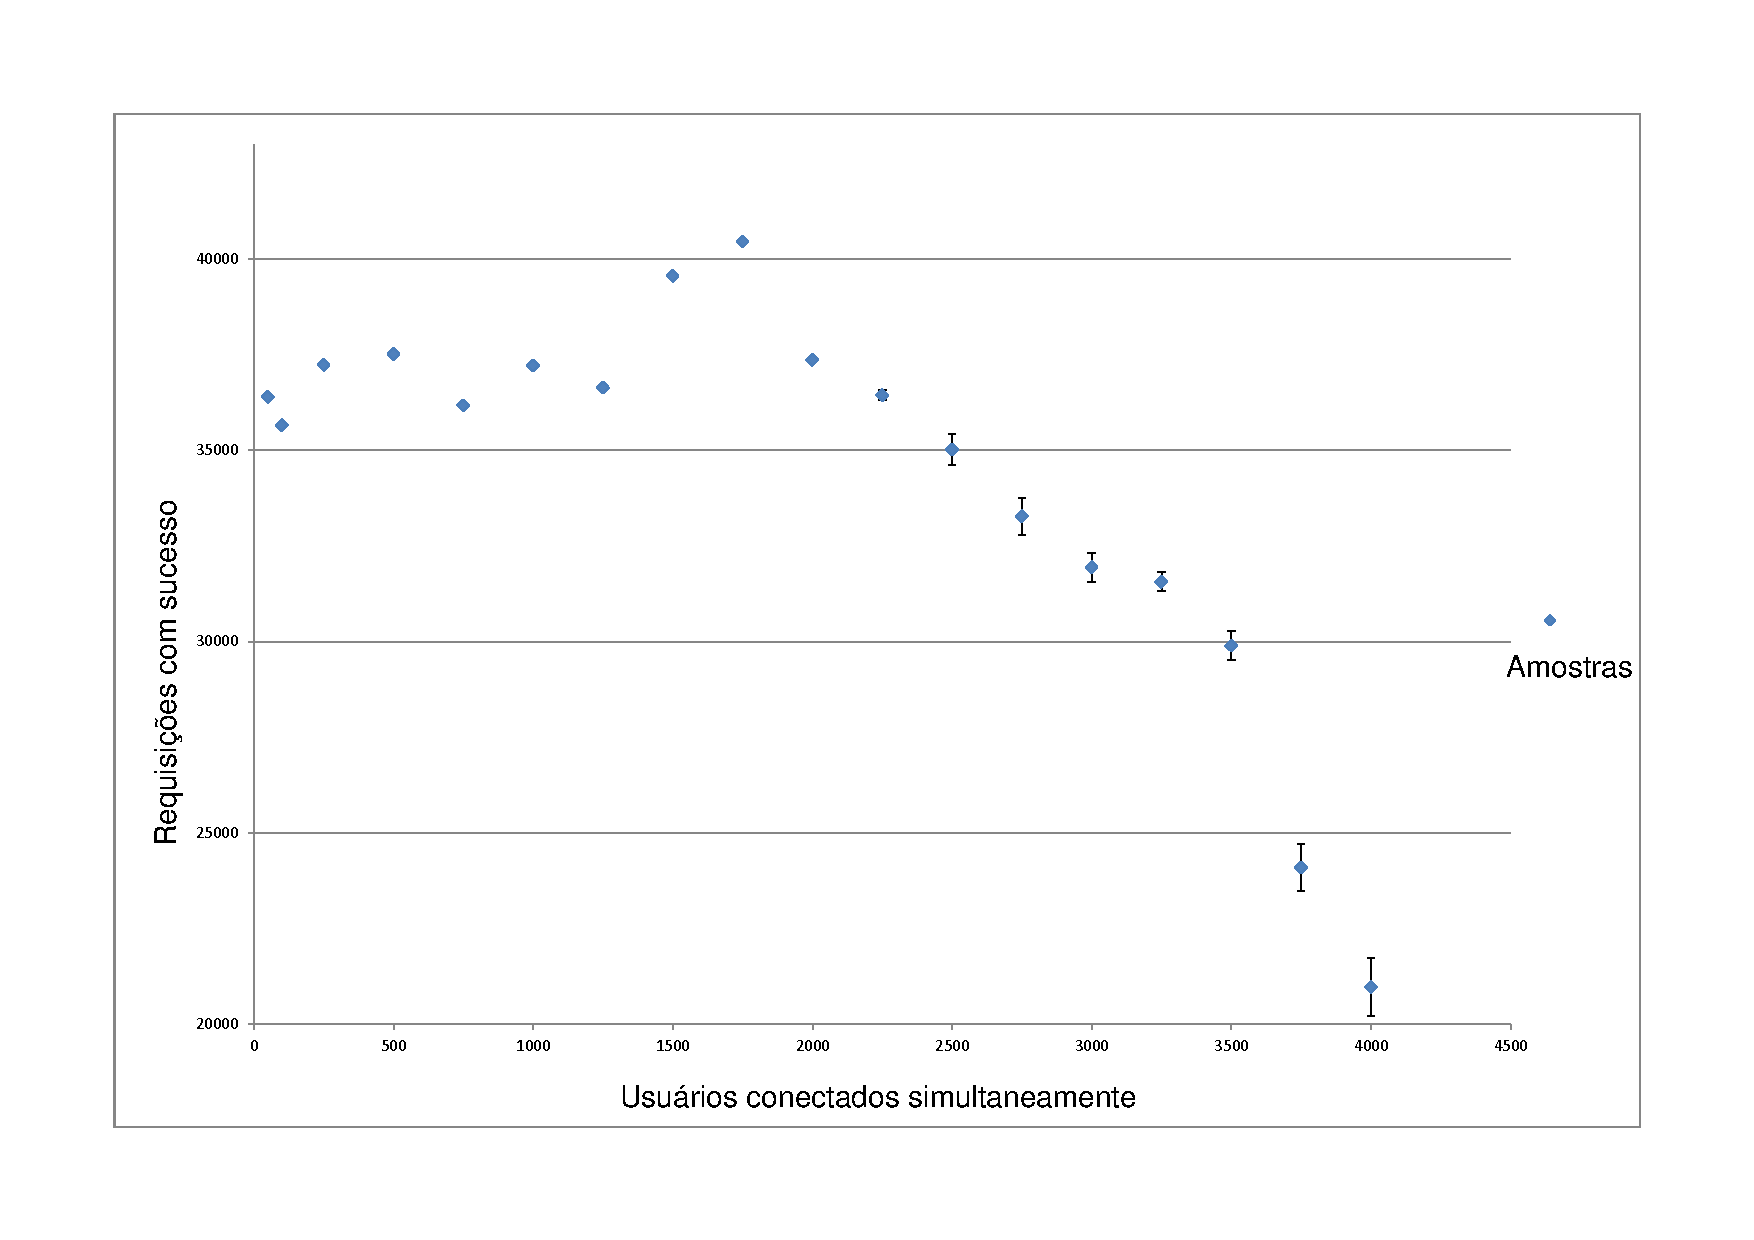
\includegraphics[scale=0.5]{imagens/dvp6.pdf}
    \caption{Média e desvio padrão do Cenário 6}
    \label{fig:dvp6}
    \end{figure}
    
Como a partir simulação com 2000 usuários praticamente todos os cenários aumentam o erro significativamente, considerou-se este o máximo que estes cenários suportam. Desta forma, plotou-se num gráfico a taxa de erro e a quantidade de requisições, onde observou-se que, nas simulações com até 2000 usuários, o erro é desconsiderável (< 0,1\%) em relação a quantidade de requisições atendidas com sucesso.

A Figura \ref{fig:max} ilustra esta simulação, cruzando total de requisições e porcentagem de erro em cada cenário, onde o erro sempre é menor que 0,1\%.    

    \begin{figure}[H]
    \centering
    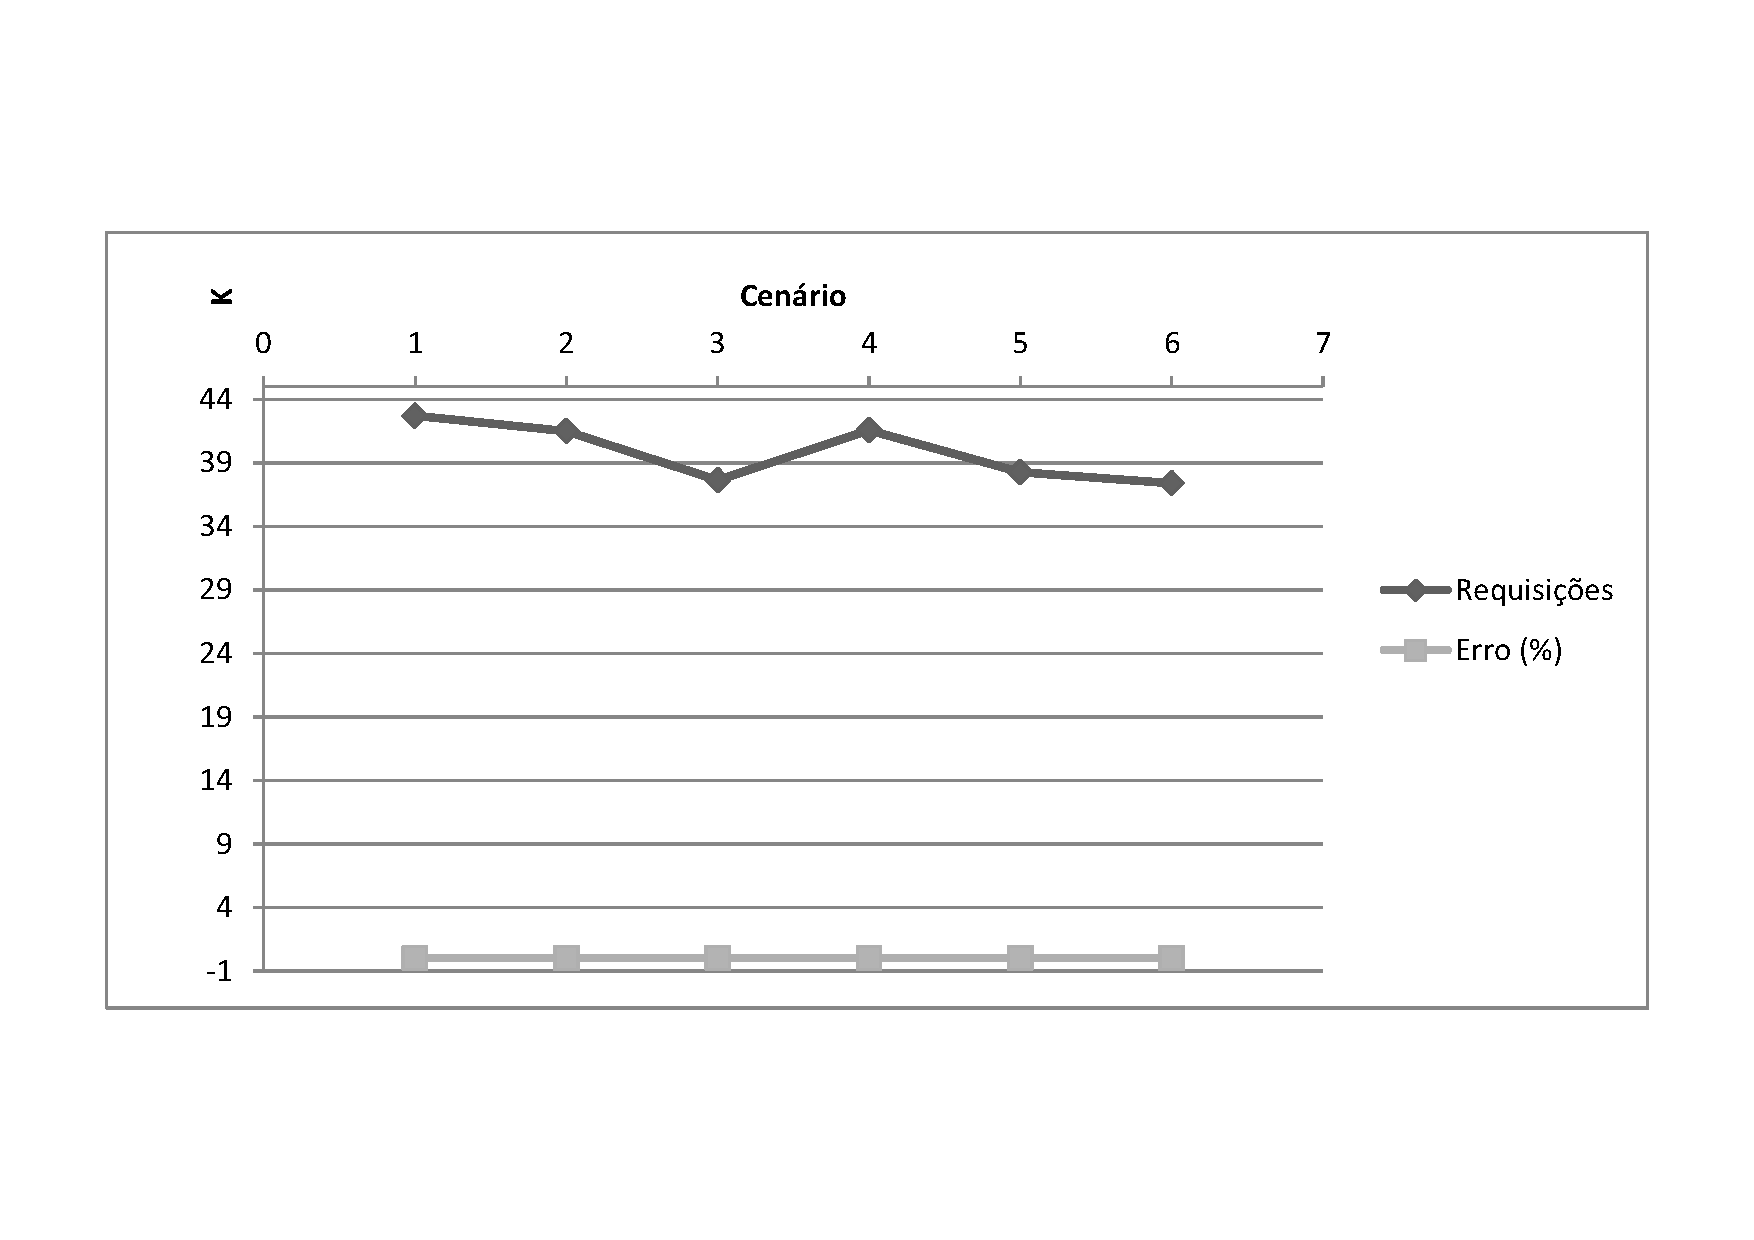
\includegraphics[scale=0.5]{imagens/reqXerro.pdf}
    \caption{Requisições e porcentagem de erro para 2000 usuários}
    \label{fig:max}
    \end{figure}

Por fim, foi estudado o impacto do uso de \textit{guests} na composição dos cenários, conforme Figura \ref{fig:lat}, que demonstrou que a latência das requisições nos cenários que não possuem \textit{guests} é menor. Porém, o uso de \textit{guests} na Computação em Nuvem traz diversos benefícios como abstração física de hardware, elasticidade, entre outros. A virtualização é o componente responsável pela característica dinâmica dos data centers. É através do uso das \textit{guests} que os ambientes virtuais de cada usuário podem ser ampliados ou reduzidos dinamicamente de maneira a atender aos recursos solicitados.  

    \begin{figure}[H]
    \centering
    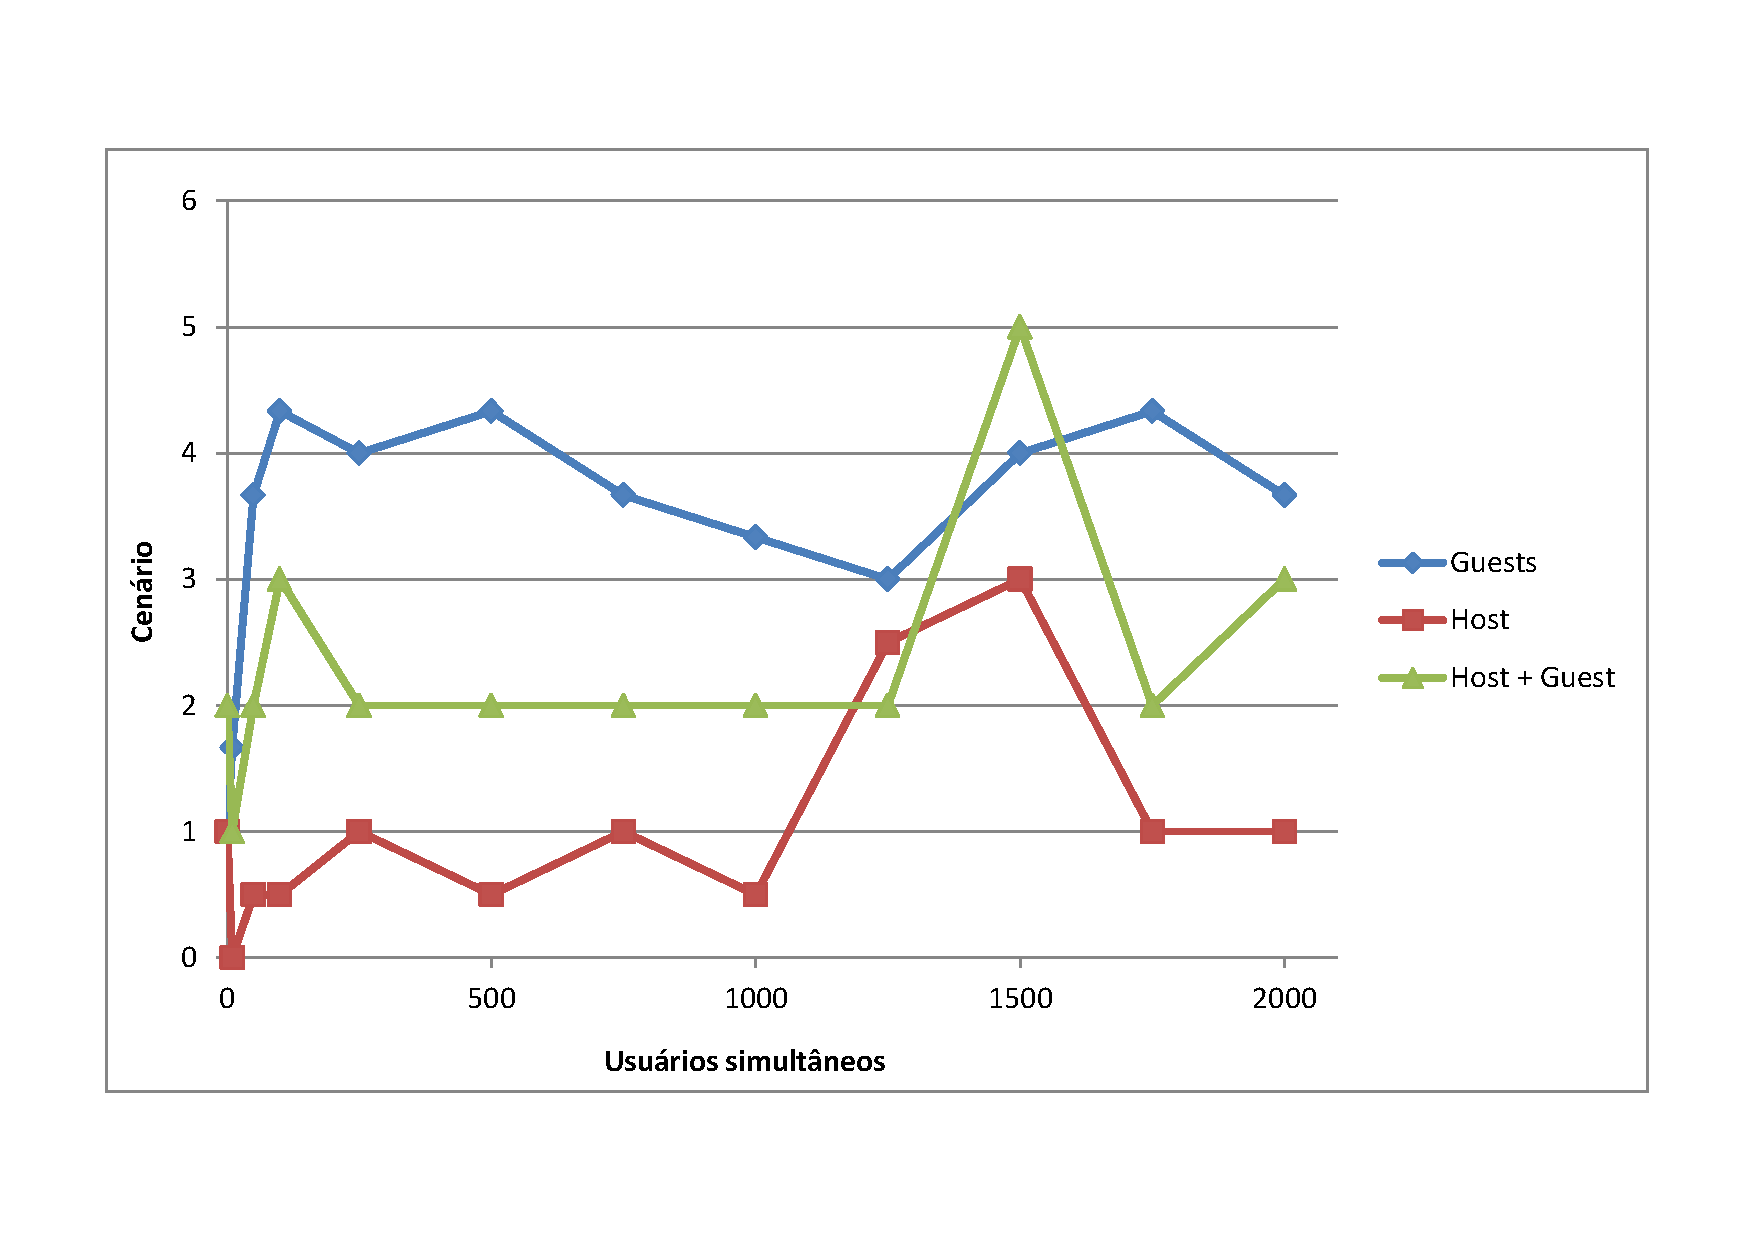
\includegraphics[scale=0.5]{imagens/latencia.pdf}
    \caption{Latência dos cenários de acordo com perfil de máquina utilizada}
    \label{fig:lat}
    \end{figure}

\section{Análise dos Resultados}
\label{sec:analResul}

Com o fim da realização das simulações e avaliação dos resultados, foi possível notar que a forma com que os cenários foram fisicamente implementados impactou na escalabilidade da base de dados. 

O Cassandra foi configurado na \textit{host} A e nesta mesma máquina foram instaladas 5 \textit{guests}. Destas, 4 eram dedicadas a base de dados e uma era responsável por executar e coletar os dados dos testes. Também havia uma \textit{host} B que fazia parte da base de dados, nos cenários em que mais de uma máquina física era necessária.

Sendo assim, sugere-se realizar em um futuro trabalho testes práticos com todas as ferramentas que o projeto Maritaca utiliza. Em especial, executar novos testes com o Cassandra, utilizando uma disposição diferente das máquinas onde a base de dados e a ferramenta responsável pelos testes estão instaladas.



%---
% dificuldades encontradas
%---
\chapter{Dificuldades Encontradas}
\label{cap:dificuldadesEncontradas}
Este capítulo descreve a complexidade da implantação de projetos distribuídos ao longo deste trabalho. Devido a esta complexidade foi necessário fazer uma revisão no objetivo inicial do trabalho que era realizar o estudo dos modelos de escalabilidade em Computação em Nuvem para o projeto Maritaca, porém acabou por ficar restrito à escalabilidade, elasticidade e robustez do banco de dados distribuído (Cassandra).


O projeto Maritaca (\textbf{MAR}itaca \textbf{I}s a \textbf{T}ool to cre\textbf{A}te \textbf{C}ellular phone \textbf{A}pplications) busca suprir as necessidades de automatizar o processo de coleta de dados móveis (CMD) provendo uma infraestrutura baseada na nuvem para criação de aplicativos móveis para \textit{smartphones} Android (\textit{apks}\footnote{Arquivos executáveis Android.}). Esses aplicativos representam os formulários digitais. O Maritaca proporciona uma \textit{interface web} interativa para a concepção do formulário e o gerenciamento das informações coletadas. O projeto possui três vertentes principais: a aplicação móvel Android, os serviços web e os repositórios de dados. 


O estudo dos modelos dependia preliminarmente do funcionamento pleno do sistema Maritaca, o que não ocorreu. Para automatizar o processo de download, instalação e configuração de pacotes essenciais para o funcionamento do sistema, foi necessário alterar o foco inicial deste trabalho para a criação de \textit{scripts} que realizassem o trabalho inicial. Porém, durante a criação destes, o projeto Maritaca demonstrou incompatibilidade de versões dos pacotes e/ou documentação deficiente do projeto com diversas distribuições Linux.

Primeiramente, foi decidido testar o processo de instalação no sistema operacional Ubuntu Server 14.04.2. Em função de diversos problemas, tentou-se utilizar outros sistemas operacionais, tais como OpenSuse 12, CentOS 7 e Fedora 21.

No OpenSuse foi detectado problemas na resolução de dependências dos pacotes utilizados pelo Maritaca. Durante a instalação dos pacotes, os mesmos apresentavam falhas em função do sistema operacional não resolver as dependências exigidas pelos pacotes.

No sistema CentOS, os pacotes exigidos pelo Maritaca foram instalados com sucesso. Porém, ao iniciar o projeto compilado, este retornara erro 404, motivo que não se conseguiu resolver.

Após o teste em diversos sistemas operacionais, descobriu-se que a versão do Maven utilizada para compilação do projeto estava com problemas na indexação dos pacotes utilizados pelo projeto. Em função disto, optou-se por alterar a versão do Maven, de 2 para 3, e reiniciou-se a criação dos scripts no sistema operacional Ubuntu Server 14.04.2.

Ainda assim, o TomCat não conseguia iniciar o projeto compilado. Por isto, iniciou-se a depuração do log do TomCat, onde detectou-se ser fundamental a criação da pasta hadoop\_mounted dentro na pasta var do sistema operacional. Porém novamente o TomCat apresentou falhas ao iniciar o projeto.

Desta forma, optou-se pela utilização do sistema operacional Fedora 21. Durante a instalação do Maven 3, verificou-se que o mesmo exigia a versão 1.8 do Java Open JDK, e ao compilar o projeto com esta versão do Java, novos problemas surgiram. Sendo assim, retomou-se a criação dos \textit{scripts} utilizando o Ubuntu Server 14.04.2.

O projeto foi então recompilado utilizando-se a versão 1.6 do Java, e iniciou-se o servidor TomCat utilizando o novo arquivo compilado, desta vez, o projeto executou com sucesso.

Ao testar a geração de aplicativos com o auxílio do Maritaca, este não conseguia gerar os \textit{apks}. Ao realizar nova depuração do log do TomCat, detectou-se a ausência de pacotes fundamentais do Android SDK para a geração dos apks. Foram então inseridos no Android SDK um conjunto de pacotes obsoletos. Testou-se novamente a geração dos apks e novo erro surgiu no log do TomCat, indicando que outras dependências do Android SDK não estavam instaladas. Instalou-se as dependências exigidas (\textit{lib32z1, lib32ncurses5, lib32bz2-1.0 e lib32stdc++6}). Com isto, a geração dos \textit{apks} pelo Maritaca passou a funcionar com sucesso.




% ---
% Finaliza a parte no bookmark do PDF, para que se inicie o bookmark na raiz
% ---
\bookmarksetup{startatroot}% 
% ---

% ---
% Conclusão
% ---
\chapter{Considerações Finais}
\label{cap:conclusoes}
Atualmente a Computação em Nuvem é utilizada principalmente por grandes serviços que surgem na internet e também por empresas
com usos particulares. Seu uso tem sido buscado e estudado principalmente pelo fato dos custos estarem sempre relacionados ao real uso dos recursos, capacidade essa possível por
sua característica elástica e adaptativa, e com o auxílio do monitoramento de seus requisitos não funcionais é possível aumentar seu valor agregado.

Essas duas características têm sido buscadas principalmente por empresas que lançam novos serviços, pois o aumento dos gastos envolvidos em seu processo de criação não é desejável. No modelo de Computação em Nuvem, a capacidade computacional pode ser ajustada de acordo com a demanda. Com isso, tem-se uma cobrança de forma mais adequada sobre os diversos perfis de clientes. A utilização de uma estrutura flexível e escalável, com melhor utilização dos recursos computacionais pode trazer consideráveis retornos financeiros para uma organização, a qual pode aproveitar a capacidade ociosa disponível e já paga e implementar novas aplicações, sem aumento dos gastos com hardware, além de que o uso de infraestrutura disponibilizada por terceiros elimina as tediosas e custosas tarefas burocráticas de gerenciar o parque tecnológico.

Com a realização deste trabalho foi possível concluir que o entendimento e configuração de sistemas que funcionam utilizando a computação em nuvem não é algo simples. Deve-se realizar um levantamento das melhores e mais estáveis ferramentas para se configurar este tipo de ambiente. É nesta etapa que são avaliados aspectos como: elasticidade, robustez, escalabilidade, estabilidade, entre outras características necessárias para a configuração, que melhor atenda os sistemas que serão hospedados.


Os projetos que dependem desta tecnologia e são desenvolvidos por pequenas ou grandes equipes precisam ser bem documentados, de forma a facilitar que um novo membro da equipe consiga entender e contribuir para a evolução do projeto. A principal dificuldade encontrada durante a realização deste trabalho foi justamente relacionada a documentação deficiente do projeto Maritaca.

As deficiências de documentação iam desde a instalação até a configuração dos \textit{softwares} necessários para que o projeto funcionasse. Com isso, surgiu a necessidade da criação de \textit{scripts} que realizassem esta tarefa automaticamente.

A elaboração destes \textit{scripts} foi a tarefa que mais demandou tempo deste trabalho de conclusão de curso e era desejável, para que fosse possível realizar testes com todas as ferramentas necessárias para o funcionamento deste sistema, de modo que, o ambiente em nuvem deste projeto fosse o mais otimizado possível para esta aplicação.

Após finalizados estes \textit{scripts} foram iniciados os testes com a base de dados Cassandra. Nestes, não foi possível avaliar a escalabilidade do Cassandra devido ao modo com que os cenários foram implementados, conforme citado na seção \ref{sec:analResul}.

Mesmo os resultados dos testes não sendo os esperados, esta foi a base de dados escolhida para o funcionamento do projeto Maritaca. Pois ele utiliza praticamente operações de escrita e atualização na base de dados e conforme ressaltado no Capítulo \ref{cap:cassandra}, o Cassandra realiza estas operações eficientemente. 

Sendo assim, sugere-se realizar em um futuro trabalho testes práticos com todas as ferramentas que o projeto Maritaca utiliza. Em especial, executar novos testes com o Cassandra, utilizando uma disposição diferente das máquinas onde a base de dados e a ferramenta responsável pelos testes estão instaladas.



% ----------------------------------------------------------
% ELEMENTOS PÓS-TEXTUAIS
% ----------------------------------------------------------
\postextual


% ----------------------------------------------------------
% Referências bibliográficas
% ----------------------------------------------------------
\bibliography{bibliografia/references}

% ----------------------------------------------------------
% Glossário
% ----------------------------------------------------------
%
% Consulte o manual da classe abntex2 para orientações sobre o glossário.
%
%\glossary

% ----------------------------------------------------------
% Apêndices
% ----------------------------------------------------------
\clearpage
% ---
% Inicia os apêndices
% ---
\begin{apendicesenv}

% Imprime uma página indicando o início dos apêndices
\partapendices

% ----------------------------------------------------------
\chapter{Scripts de Instalação e Configuração}
% ----------------------------------------------------------
Os arquivos \textit{install.sh, download.sh, configurate.sh, start.sh, stop.sh, automacao.sh, cassandra\_keyspace.txt, configuration.properties, apt.conf, setenv.sh e solr.xml} fazem parte do processo de automação de funcionamento do projeto Maritaca, citado no Capítulo \ref{cap:dificuldadesEncontradas}.

\section*{install.sh}
\begin{lstlisting}[style=Bash]
#!/bin/bash

#Pre-Requisito: Ter o git instalado
#sudo apt-get install -y git

cd
exec 5> debug_install.txt
BASH_XTRACEFD="5"
set -x

################ VARIABLES ##################
JAVA_REPOSITORY="ppa:webupd8team/java"
FFMPEG_REPOSITORY="ppa:mc3man/trusty-media"

################ FUNCTIONS ##################
repository_local(){
cd
sudo cp -r -p maritaca-code/doc/scripts/apt.conf /etc/apt/
}

repository_add(){
sudo add-apt-repository -y $JAVA_REPOSITORY
sudo add-apt-repository -y $FFMPEG_REPOSITORY
}

repository_update(){
sudo apt-get update
}

softwares_install(){
sudo apt-get install -y oracle-java6-installer # Java 7 da erro no sdk android
sudo apt-get install -y oracle-java6-set-default
sudo apt-get install -y libjna-java
sudo apt-get install -y python-software-properties # Dependencias cassandra
sudo apt-get install -y curl # Dependencias cassandra
sudo apt-get install -y ant
sudo apt-get install -y xvfb
sudo apt-get install -y maven
sudo apt-get install -y lynx
sudo apt-get install -y rabbitmq-server
sudo apt-get install -y ffmpeg
sudo apt-get install -y lib32z1 lib32ncurses5 lib32bz2-1.0 lib32stdc++6 #Dependencias do android SDK
sudo apt-get install -y apache2
}

#repository_local
repository_add
repository_update
softwares_install
\end{lstlisting}

\section*{download.sh}
\begin{lstlisting}[style=Bash]
#!/bin/bash

exec 5> debug_download.txt
BASH_XTRACEFD="5"
set -x

pcts_download(){
	cd 

	if [ -e "cassandra.tgz" ] ; then
		echo "Cassandra Já Baixado"
	else
		wget -O cassandra.tgz http://ftp.unicamp.br/pub/apache/cassandra/1.2.19/apache-cassandra-1.2.19-bin.tar.gz >> debug_download.txt
	fi

	if [ -e "tomcat7.tgz" ] ; then
		echo "Tomcat Já Baixado"
	else	
		wget -O tomcat7.tgz http://ftp.unicamp.br/pub/apache/tomcat/tomcat-7/v7.0.61/bin/apache-tomcat-7.0.61.tar.gz >> debug_download.txt
	fi

	if [ -e "solr.tgz" ] ; then
		echo "Solr Já Baixado"
	else
		wget -O solr.tgz http://archive.apache.org/dist/lucene/solr/4.2.0/solr-4.2.0.tgz >> debug_download.txt
	fi

	if [ -e "android.tgz" ] ; then
		echo "Android Já Baixado"
	else
		wget -O android.tgz http://dl.google.com/android/android-sdk_r22.3-linux.tgz >> debug_download.txt
	fi
}

pcts_extract(){
	cd 
	tar zxvf cassandra.tgz 
	tar zxvf tomcat7.tgz 
	tar zxvf solr.tgz 
	tar zxvf android.tgz 
}

pcts_rename_folder(){
	cd 
	mv apache-cassandra-1.2.19/ cassandra 
	mv apache-tomcat-7.0.61/ tomcat 
	mv solr-4.2.0/ solr42 
	mv android-sdk-linux/ androidSDK 
}

pcts_download
pcts_extract
pcts_rename_folder
\end{lstlisting}

\section*{configurate.sh}
\begin{lstlisting}[style=Bash]
#!/bin/bash

exec 5> debug_configurate.txt
BASH_XTRACEFD="5"
set -x

project_clone(){
	cd 
	git clone http://git.code.sf.net/p/maritaca/code maritaca-code 
}

project_build(){
	cd 
	maritaca-code/server/ 
	mvn clean install -Dmaven.test.skip=true
	cd
	maritaca-code/services/rabbit-consumer/
	mvn clean install
}

pcts_copy_folders(){
	cd 

	#ARQUIVOS DE CONFIGURAÇÃO DO SOLR
	cp -r tomcat/ solr42/ 
	mkdir -p solr42/solr/data 
	mkdir -p solr42/tomcat/conf/Catalina/localhost 
	cp maritaca-code/doc/scripts/solr.xml solr42/tomcat/conf/Catalina/localhost/solr.xml
	cp maritaca-code/doc/scripts/setenv.sh tomcat/bin/setenv.sh 
	cp solr42/dist/solr-4.2.0.war solr42/solr/solr.war 
	cp -r -p solr42/example/solr/* solr42/solr/data/.
	cp -p maritaca-code/server/search/src/main/resources/schema.xml solr42/solr/data/collection1/conf/schema.xml

	#ARQUIVO - VARIAVEIS DE AMBIENTE
	sudo cp -r -p maritaca-code/doc/scripts/configuration.properties /opt/

	#ARQUIVO COM APONTAMENTO DA VARIAVEL DE AMBIENTE P/ TOMCAT
	cp maritaca-code/doc/scripts/setenv.sh tomcat/bin/setenv.sh

	#COPIA DO maritaca.war gerado após build de projeto
	sudo cp -r -p maritaca-code/server/web/target/maritaca.war tomcat/webapps/ 

	#DIRETÓROS HADOOP
	mkdir -p hadoop_mounted/user/maritaca/{apk,audio,picture,video} 

	#DIRETÓRIO APPS
	mkdir -p maritaca-code/client/apps 
	
	#COPIA DOS ARQUIVOS COM SUAS RESPECTIVAS PERMISSÕES PARA A PASTA /OPT
	sudo cp -r -p tomcat/ /opt/ 
	sudo cp -r -p solr42/ /opt/ 
	sudo cp -r -p cassandra/ /opt/ 
	sudo cp -r -p hadoop_mounted/ /var/www/ 
	sudo cp -r -p androidSDK/ /opt/
	sudo cp -r -p maritaca-code/ /opt/
}

configurate_cassandra(){
	cd 
	sudo /opt/cassandra/bin/cassandra
	sleep 10
	sudo /opt/cassandra/bin/cassandra-cli -h localhost -port 9160 -f maritaca-code/doc/scripts/cassandra_keyspace.txt 
	#sudo /opt/cassandra/bin/stop-server 
}

configurate_rabbitMQ(){
	sudo rabbitmqctl add_user maritaca maritaca 
	sudo rabbitmqctl add_vhost Maritaca 
	sudo rabbitmqctl set_permissions -p Maritaca maritaca ".*" ".*" ".*" 
}

configurate_solr42(){
	perl -i -pe 's/<Server port="8005" shutdown="SHUTDOWN">/<Server port="8105" shutdown="SHUTDOWN">/' /opt/solr42/tomcat/conf/server.xml 
	perl -i -pe 's/<Connector port="8080" protocol="HTTP/<Connector port="8983" protocol="HTTP/' /opt/solr42/tomcat/conf/server.xml 
	perl -i -pe 's/<Connector port="8009" protocol="AJP/<Connector port="8109" protocol="AJP/' /opt/solr42/tomcat/conf/server.xml 
	perl -i -pe 's/{solr.data.dir:}/{solr.data.dir:\/opt\/solr42\/solr\/data}/' /opt/solr42/solr/data/collection1/conf/solrconfig.xml 
}

#configurate_tomcat(){
	perl -i -pe 's/redirectPort="8443"/redirectPort="8443" URIEncoding="UTF-8"/' /opt/tomcat/conf/server.xml

#}

configurate_androidSDK(){
	/opt/androidSDK/tools/android list sdk 
	/opt/androidSDK/tools/android update sdk -u --all
}

##################################   CODE    ################################## 

#project_clone
project_build

pcts_copy_folders

configurate_cassandra
configurate_rabbitMQ
configurate_solr42
configurate_tomcat
configurate_androidSDK
\end{lstlisting}

\section*{start.sh}
\begin{lstlisting}[style=Bash]
#!/bin/bash

exec 5> debug_start.txt
BASH_XTRACEFD="5"

iniciar_servicos(){
	#sudo service apache2 start #para quando apache não inicia automaticamente com SO
	sudo service apache2 status
	sleep 5
	#sudo service rabbitmq-server start #para quando rabbitmq-server não inicia automaticamente com SO
	sudo service rabbitmq-server status
	sleep 5
	sudo /opt/cassandra/bin/cassandra
	sleep 5
	sudo /opt/solr42/tomcat/bin/startup.sh
	sleep 5 
	sudo /opt/tomcat/bin/startup.sh
	sleep 5
	java -jar /opt/maritaca-code/services/rabbit-consumer/target/rabbit-consumer-1.0.jar &
	sleep 5
	lynx http://localhost:8080/maritaca
}

iniciar_servicos
\end{lstlisting}

\section*{stop.sh}
\begin{lstlisting}[style=Bash]
#!/bin/bash

exec 5> debug_stop.txt
BASH_XTRACEFD="5"

parar_servicos(){
	sudo service apache2 stop
	sleep 5
	sudo service apache2 status
	sudo service rabbitmq-server stop
	sleep 5
	sudo service rabbitmq-server status
	#sudo /opt/cassandra/bin/stop-server 
	sudo /opt/solr42/tomcat/bin/shutdown.sh
	sleep 5
	sudo /opt/tomcat/bin/shutdown.sh 
}

parar_servicos
\end{lstlisting}

\section*{automacao.sh}
\begin{lstlisting}[style=Bash]
#!/bin/bash

cd
maritaca-code/doc/scripts/install.sh
maritaca-code/doc/scripts/download.sh
maritaca-code/doc/scripts/configurate.sh
maritaca-code/doc/scripts/start.sh
\end{lstlisting}

\section*{cassandra\_keyspace.txt}
\begin{lstlisting}[style=Bash]
create keyspace Maritaca;
exit;
\end{lstlisting}

\section*{configuration.properties}
\begin{lstlisting}[style=Bash]
maritaca_mobile_path=/opt/maritaca-code/client/
android_sdk_path=/opt/androidSDK
maritaca_uri_server=http://localhost:8080/maritaca

filesystem_path=/var/www/hadoop_mounted/user/maritaca
http_uri_server=http://localhost/hadoop_mounted/user/maritaca/

ffmpeg_path=/opt/ffmpeg
tmp_directory=/tmp/

cluster_addr=localhost:9160
\end{lstlisting}

\section*{apt.conf}
\begin{lstlisting}[style=Bash]
Acquire::http::Proxy "http://mrt00:3142";
Acquire::ftp::Proxy "http://mrt00:3142";
\end{lstlisting}

\section*{setenv.sh}
\begin{lstlisting}[style=Bash]
#! /bin/sh

export MARITACA_CONFIG_PATH="/opt/configuration.properties"
\end{lstlisting}


\section*{solr.xml}
\begin{lstlisting}[style=xml]
<Context docBase="/opt/solr42/solr/solr.war" debug="0" crossContext="true">
	<Environment name="solr/home" type="java.lang.String" value="/opt/solr42/solr/data" override="true"/>
</Context>	
\end{lstlisting}


\chapter{JMeter e CassJMeter - \textit{xml} gerado para os testes}

Após a ferramente ser configurada, é possível visualizar os parâmetros utilizados no teste através de um arquivo \textit{.xml} gerado pelo próprio JMeter. O arquivo \textit{Cenario1.jmx} exibe os parâmetros utilizados nos testes do Cenário 1 com um usuário. 

\section*{Cenario1.jmx}
\begin{lstlisting}[style=xml]
<?xml version="1.0" encoding="UTF-8"?>
<jmeterTestPlan version="1.2" properties="2.4" jmeter="2.9 r1437961">
  <hashTree>
    <TestPlan guiclass="TestPlanGui" testclass="TestPlan" testname="Testes Cassandra" enabled="true">
      <stringProp name="TestPlan.comments"></stringProp>
      <boolProp name="TestPlan.functional_mode">false</boolProp>
      <boolProp name="TestPlan.serialize_threadgroups">true</boolProp>
      <elementProp name="TestPlan.user_defined_variables" elementType="Arguments" guiclass="ArgumentsPanel" testclass="Arguments" testname="User Defined Variables" enabled="true">
        <collectionProp name="Arguments.arguments"/>
      </elementProp>
      <stringProp name="TestPlan.user_define_classpath"></stringProp>
      <boolProp name="TestPlan.tearDown_on_shutdown">true</boolProp>
    </TestPlan>
    <hashTree>
      <ThreadGroup guiclass="ThreadGroupGui" testclass="ThreadGroup" testname="Grupo de Usuários" enabled="true">
        <stringProp name="ThreadGroup.on_sample_error">continue</stringProp>
        <elementProp name="ThreadGroup.main_controller" elementType="LoopController" guiclass="LoopControlPanel" testclass="LoopController" testname="Loop Controller" enabled="true">
          <boolProp name="LoopController.continue_forever">false</boolProp>
          <intProp name="LoopController.loops">-1</intProp>
        </elementProp>
        <stringProp name="ThreadGroup.num_threads">1</stringProp>
        <stringProp name="ThreadGroup.ramp_time">1</stringProp>
        <longProp name="ThreadGroup.start_time">1434586680000</longProp>
        <longProp name="ThreadGroup.end_time">1434586740000</longProp>
        <boolProp name="ThreadGroup.scheduler">true</boolProp>
        <stringProp name="ThreadGroup.duration">60</stringProp>
        <stringProp name="ThreadGroup.delay">10</stringProp>
        <boolProp name="ThreadGroup.delayedStart">true</boolProp>
      </ThreadGroup>
      <hashTree>
        <com.netflix.jmeter.properties.CassandraProperties guiclass="TestBeanGUI" testclass="com.netflix.jmeter.properties.CassandraProperties" testname="MyTestCluster" enabled="true">
          <stringProp name="cassandraServers">172.22.164.5:9160</stringProp>
          <stringProp name="clientType">com.netflix.jmeter.connections.thrift.ThriftConnection</stringProp>
          <stringProp name="clusterName">Maritaca Cluster</stringProp>
          <stringProp name="keyspace">OpsCenter</stringProp>
          <stringProp name="maxConnsPerHost">100</stringProp>
          <stringProp name="readConsistency">ONE</stringProp>
          <stringProp name="writeConsistency">ONE</stringProp>
        </com.netflix.jmeter.properties.CassandraProperties>
        <hashTree/>
        <com.netflix.jmeter.sampler.PutSampler guiclass="com.netflix.jmeter.gui.Put" testclass="com.netflix.jmeter.sampler.PutSampler" testname="Cassandra Put" enabled="true">
          <stringProp name="TestPlan.comments">test comment</stringProp>
          <stringProp name="KEY_SERIALIZER_TYPE">StringSerializer</stringProp>
          <stringProp name="KEY">${__Random(1,1000)}</stringProp>
          <stringProp name="COLUMN_FAMILY">events</stringProp>
          <stringProp name="COLUMN_SERIALIZER_TYPE">AsciiSerializer</stringProp>
          <stringProp name="VALUE_SERIALIZER_TYPE">AsciiSerializer</stringProp>
          <stringProp name="COLUMN_NAME">${__Random(1,1000)}</stringProp>
          <stringProp name="VALUE">${__Random(1,1000)}</stringProp>
          <boolProp name="IS_COUNTER">false</boolProp>
        </com.netflix.jmeter.sampler.PutSampler>
        <hashTree/>
        <ResultCollector guiclass="SummaryReport" testclass="ResultCollector" testname="Summary Report" enabled="true">
          <boolProp name="ResultCollector.error_logging">false</boolProp>
          <objProp>
            <name>saveConfig</name>
            <value class="SampleSaveConfiguration">
              <time>true</time>
              <latency>true</latency>
              <timestamp>true</timestamp>
              <success>true</success>
              <label>true</label>
              <code>true</code>
              <message>true</message>
              <threadName>true</threadName>
              <dataType>true</dataType>
              <encoding>false</encoding>
              <assertions>true</assertions>
              <subresults>true</subresults>
              <responseData>false</responseData>
              <samplerData>false</samplerData>
              <xml>false</xml>
              <fieldNames>false</fieldNames>
              <responseHeaders>false</responseHeaders>
              <requestHeaders>false</requestHeaders>
              <responseDataOnError>false</responseDataOnError>
              <saveAssertionResultsFailureMessage>false</saveAssertionResultsFailureMessage>
              <assertionsResultsToSave>0</assertionsResultsToSave>
              <bytes>true</bytes>
            </value>
          </objProp>
          <stringProp name="filename"></stringProp>
        </ResultCollector>
        <hashTree/>
      </hashTree>
    </hashTree>
  </hashTree>
</jmeterTestPlan>

\end{lstlisting}

\end{apendicesenv}
% ---



% ----------------------------------------------------------
% Anexos
% ----------------------------------------------------------
%\clearpage
%% ---
% Inicia os anexos
% ---
\begin{anexosenv}

% Imprime uma página indicando o início dos anexos
\partanexos

    

% ---

\end{anexosenv}


\end{document}